% ============================================================================
%  Compile this file and nothing else.
%    util/include.tex   packages
%    util/format.tex    macros and notation
%    sections/*.tex     one file per section, flat, numeric prefix
%    figures/           generated by Code/Figures, never hand-edited
%    tables/            generated tabular fragments
%  No .tex file in this project may contain a parent-directory path.
%  Class and bst come from the IEEE template kept in reference/.
%  EDITOR INVARIANT: main.tex is the sole build root. Preserve -synctex=1,
%  build/main.pdf, and reverse SyncTeX when changing this project structure.
% ============================================================================

\documentclass[conference]{IEEEtran}
\IEEEoverridecommandlockouts
% The preceding line is only needed to identify funding in the first footnote.
% If that is unneeded, comment it out.
% Page numbers (Dirk 2026-10-21): the conference option blanks the header, the
% only place IEEEtran prints the page number; plain puts it centred in the footer.
\pagestyle{plain}
\makeatletter\let\ps@IEEEtitlepagestyle\ps@plain\makeatother

% include.tex  --  packages only. No macros, no styling here.
% Base set is the one shipped with IEEE-conference-template-062824.tex.

\usepackage{cite}
\usepackage{amsmath,amssymb,amsfonts}
\usepackage{algorithmic}
\usepackage{graphicx}
\usepackage{textcomp}
\usepackage{xcolor}

% Added for this paper.
\usepackage{bm}
\usepackage{booktabs}
\usepackage{placeins}   % \FloatBarrier: keeps the Results floats in their own subsection (Dirk 2026-10-24)
\usepackage{array}
\usepackage{subcaption}
\usepackage{url}
\usepackage[hidelinks]{hyperref}
\usepackage{microtype}
\usepackage{tikz}
\usetikzlibrary{arrows.meta,calc,decorations.pathmorphing}
\usepackage[normalem]{ulem}   % \sout for the feedback-change marks (format.tex); normalem keeps \emph italic

% LaTeX never looks outside Writing/. Figures are build artefacts produced by
% Figure scripts under Code/Figures generate these assets; they are never hand-edited.
\graphicspath{{figures/}}

% format.tex  --  macros, notation, styling. Swap the class without touching this.

\def\BibTeX{{\rm B\kern-.05em{\sc i\kern-.025em b}\kern-.08em
    T\kern-.1667em\lower.7ex\hbox{E}\kern-.125emX}}

% ---------------------------------------------------------------- review preview
% Uncomment to make the editor build (main.pdf) show what supervisors see: no todos,
% no wip blocks, outlines as plain bullets. Comment out again to get the working version.
%\def\ReviewBuild{}

% ---------------------------------------------------------------- draft switch
% \drafttrue  -> todo notes visible.   \draftfalse -> submission build.
\newif\ifdraft
\drafttrue
\ifdefined\ReviewBuild\draftfalse\fi   % review.tex defines \ReviewBuild: review PDF for supervisors
\ifdraft
  \newcommand{\todo}[1]{\textcolor{red}{[\textbf{TODO:} #1]}}
  \newcommand{\note}[1]{\textcolor{blue}{[#1]}}
  \newcommand{\kw}[1]{\textcolor{teal}{#1}}   % keep-word: fixed term during own-words rewrite
\else
  \newcommand{\todo}[1]{}
  \newcommand{\note}[1]{}
  \newcommand{\kw}[1]{#1}                     % submission build: plain text
\fi

% ---------------------------------------------------------------- review switch
% wip:     text kept in the file but not shown to supervisors (old bullets, AI prose).
%          \begin{wip} and \end{wip} each on their own line (comment package).
% outline: the clean bullets of what a section will state. A list: write \item lines.
% main.tex (editor build): wip shown, outline shown in blue.
% review.tex (review build): wip removed, outline shown as a plain list, todos removed.
\usepackage{comment}
\ifdefined\ReviewBuild
  \excludecomment{wip}
  \newenvironment{outline}{\begin{itemize}}{\end{itemize}}
  % review: cite the source only, without the Eq./Sec./Thm. part in brackets
  \let\fullcite\cite
  \renewcommand{\cite}[2][]{\fullcite{#2}}
\else
  \includecomment{wip}
  \newenvironment{outline}{\begingroup\color{blue!60!black}\begin{itemize}}{\end{itemize}\endgroup}
\fi
% \ucite: a citation whose source is not yet checked. Editor build: normal citation in orange.
% Review build: no citation, and the source is left out of the reference list.
% Same arguments as \cite; change back to \cite once the source is checked.
\ifdefined\ReviewBuild
  \newcommand{\ucite}[2][]{}
\else
  \newcommand{\ucite}[2][]{{\color{orange}\if\relax\detokenize{#1}\relax\cite{#2}\else\cite[#1]{#2}\fi}}
\fi
% \revnote: a remark for supervisors. Shown in main.tex and review.tex, removed at submission.
\ifdefined\ReviewBuild
  \newcommand{\revnote}[1]{\textcolor{violet}{[\textbf{Note:} #1]}}
\else\ifdraft
  \newcommand{\revnote}[1]{\textcolor{violet}{[\textbf{Note:} #1]}}
\else
  \newcommand{\revnote}[1]{}
\fi\fi

% ------------------------------------------------------------ feedback changes
% Marks for revising text after supervisor feedback (2026-10-18). Black text is the
% original word for word. Editor build: changes visible. Review and submission build:
% final text only, deletions gone, no tags. [tag] is the comment id, e.g. Jan3, Js12, Q5.
%   \chg[tag]{old}{new}   word-level fix: old struck grey, new green
%   \del[tag]{text}       deleted text: struck grey
%   \add[tag]{text}       new text: green
%   \mv[tag]{P3}          before a moved sentence: grey tag "P3" (paragraph it came from)
%   \changelegend         one-line legend, put once at the top of a revised section
% \showdeletionsfalse hides the struck text to read the revised flow.
\newif\ifshowdeletions
\showdeletionstrue
\definecolor{chgnew}{rgb}{0,0.45,0.15}
\newcommand{\fbtag}[1]{\if\relax\detokenize{#1}\relax\else\textsuperscript{\tiny\color{gray}#1}\fi}
% \fbsout: grey strikethrough; boxes \cite, which \sout cannot break into
\newcommand{\fbsout}[1]{{\color{gray}\let\fbcite\cite\def\cite##1{\mbox{\fbcite{##1}}}\sout{#1}}}
\ifdraft
  \newcommand{\chg}[3][]{\ifshowdeletions\fbsout{#2}\ \fi{\color{chgnew}#3}\fbtag{#1}}
  \newcommand{\del}[2][]{\ifshowdeletions\fbsout{#2}\fbtag{#1}\fi}
  \newcommand{\add}[2][]{{\color{chgnew}#2}\fbtag{#1}}
  \newcommand{\mv}[2][]{\textsuperscript{\tiny\color{gray}from #2\if\relax\detokenize{#1}\relax\else, #1\fi}\,}
  \newcommand{\changelegend}{{\footnotesize\color{gray}[Changes: black = original,
    {\color{chgnew}green} = changed or new, \sout{struck} = deleted,
    \textsuperscript{\tiny from P3} = moved from paragraph 3, superscript = comment id.]}\par}
\else
  \newcommand{\chg}[3][]{#3}
  \newcommand{\del}[2][]{}
  \newcommand{\add}[2][]{#2}
  \newcommand{\mv}[2][]{}
  \newcommand{\changelegend}{}
\fi

% ------------------------------------------------------------ general notation
% Copied verbatim from scripts/gantry/orthogonal-by-construction/documentation/
% state-level-obc-derivation.tex so the two documents stay comparable.
\newcommand{\R}{\mathbb{R}}
\newcommand{\ran}{\operatorname{range}}
\newcommand{\rank}{\operatorname{rank}}
\newcommand{\col}{\operatorname{col}}
\newcommand{\norm}[1]{\left\lVert#1\right\rVert}
\newcommand{\code}[1]{\nolinkurl{#1}}

% ------------------------------------------------------------ paper notation
% Define the symbols for this paper here, once.
% Section II: gantry coordinates, baseline model, LFR.
\newcommand{\qact}{q_{\mathrm{act}}}     % actuator coordinates [X1 X2 Y]^T
\newcommand{\uact}{u_{\mathrm{act}}}     % actuator forces
\newcommand{\fnet}{f_{\mathrm{net}}}     % net generalized force on the inertia
\newcommand{\Dsch}{\Delta}               % scheduling block of the LFR


\begin{document}

% TU/e AI&ES cover from the official open-access LaTeX template, ASMPT logo added (Dirk 2026-10-18).
% cover.tex  --  TU/e AI&ES MSc thesis cover (open access), rebuilt in LaTeX
% 1:1 from frontmatter/titlepage.pdf (Dirk 2026-10-18). Every position, font
% and size is taken from the template's text baselines (PDF bp from the
% bottom-left corner of the A4 template). The TU/e logo is cropped from the
% template itself; the ASMPT logo is added top left. Only deviation: Program
% needs two lines, so the Graduation rows below it move down one line.

\newcommand{\coverat}[3]{% x, baseline y, text (left aligned)
  \node[anchor=base west] at (#1bp,#2bp) {#3};}
\newcommand{\coverline}[3]{% x, baseline y, width: template form line
  \fill (#1bp,#2bp-1.56bp) rectangle ++(#3,-0.48bp);}
\newlength{\coverdate}
\settowidth{\coverdate}{\fontsize{9.96}{12}\selectfont 17 November 2026}
\ifdim\coverdate<56.4bp \setlength{\coverdate}{56.4bp}\fi

\begin{titlepage}
\begin{tikzpicture}[remember picture, overlay,
    every node/.style={inner sep=0bp, outer sep=0bp}]
  % The A4 template (595.56 x 842.04 bp) is fitted to the US Letter IEEEtran
  % page (612 x 792 bp) as pdfpages would: scale 792/842.04, centred.
  \begin{scope}[shift={(current page.south west)},
      xshift=25.91bp, scale=0.940573, transform shape]

  % Logos.
  \node[anchor=west] at (72bp,751.5bp)
    {\includegraphics[height=24bp]{frontmatter/asmpt_logo.png}};
  \node[anchor=south west] at (364.65bp,730.99bp)
    {\includegraphics[viewport=364.65 730.99 515.36 772.04, clip]
      {frontmatter/titlepage.pdf}};

  \fontsize{9.96}{12}\selectfont
  \coverat{81.96}{684.12}{\bfseries Department of Electrical Engineering}

  % Title block, each line centred where the template placeholder was centred.
  \node[anchor=base] at (276.5bp,537bp)
    {\fontsize{17.04}{20}\selectfont\bfseries Model Augmentation for a};
  \node[anchor=base] at (276.5bp,517bp)
    {\fontsize{17.04}{20}\selectfont\bfseries High-Precision Dual-Drive Gantry};
  \coverat{277.56}{487.08}{\fontsize{12}{14}\selectfont by}
  \node[anchor=base] at (279.8bp,442.91bp)
    {\fontsize{14.04}{16}\selectfont\bfseries D.J.L.M. van den Berg};
  \coverat{251.52}{356.40}{\fontsize{14.04}{16}\selectfont MSc Thesis}

  % Thesis committee (fifth line left empty).
  \coverat{72}{300.36}{\bfseries Thesis committee}
  \coverat{72}{285}{dr.\ ir.\ M. Schoukens}
  \coverat{72}{273}{prof.\ dr.\ ir.\ R. T{\'o}th}
  \coverat{72}{261}{dr.\ ir.\ M.F. Shakib}
  \coverat{72}{247.8}{ir.\ J. Gerritsen}

  % Graduation. Template baselines; rows after Program shifted by 11.88 bp.
  \coverat{304.35}{300.36}{\bfseries Graduation}
  \coverat{304.35}{284.88}{Program:}
  \coverat{395.76}{284.52}{Artificial Intelligence and}
  \coverat{395.76}{272.64}{Engineering Systems}
  \coverat{304.35}{261.12}{Capacity group:}
  \coverat{395.76}{260.52}{Control Systems}
  \coverat{304.35}{249.24}{Thesis supervisor:}
  \coverat{395.76}{247.92}{dr.\ ir.\ M. Schoukens}
  \coverat{304.34}{236.40}{Date of defense:}
  \coverat{396}{236.40}{17 November 2026}
  \coverline{396}{236.40}{\coverdate}
  \coverat{304.32}{224.76}{Student ID:}
  \coverat{395.4}{224.76}{1555561}
  \coverline{395.4}{224.76}{57bp}
  \coverat{304.32}{213.12}{Study load (ECTS):}
  \coverat{395.76}{213.12}{45}
  \coverline{395.76}{213.12}{56.64bp}
  \coverat{304.32}{200.52}{Track:}
  \coverat{395.39}{200.52}{High-Tech Systems and Robotics}

  % Footer, line by line; full lines are spread to the template text width.
  \coverat{71.28}{149.28}{The research of this thesis has been carried out
    in collaboration with \textit{ASMPT, Beuningen}.}
  \coverat{71.88}{136.80}{\fontfamily{ppl}\fontsize{9.02}{11}\selectfont
    This thesis is public and Open Access.}
  \coverat{71.28}{113.40}{\makebox[444.3bp][s]{This thesis has been realized
    in accordance with the regulations as stated in the TU/e Code of
    Scientific}}
  \coverat{71.28}{101.88}{Conduct.}
  \coverat{71.28}{78.24}{\makebox[444.3bp][s]{Disclaimer: the Department of
    Electrical Engineering of the Eindhoven University of Technology accepts
    no}}
  \coverat{71.28}{66.72}{responsibility for the contents of MSc theses or
    practical training reports.}
  \end{scope}
\end{tikzpicture}
\end{titlepage}


\title{Model Augmentation for a High-Precision Dual-Drive Gantry
%Model Augmentation for a Dual-Gantry High-Precision Motion System
% \thanks{Identify applicable funding agency here. If none, delete this.}}
}
\author{\IEEEauthorblockN{Dirk van den Berg}
\IEEEauthorblockA{\textit{Control Systems Group, Dept. of Electrical Engineering} \\
\textit{Eindhoven University of Technology}\\
Eindhoven, The Netherlands\\
In collaboration with \textit{ASMPT}, Beuningen, The Netherlands\\[1ex]
Supervisors: dr.\ ir.\ M. Schoukens, prof.\ dr.\ ir.\ R. T{\'o}th,
ir.\ J.H. Hoekstra (TU/e);\\
ir.\ Q. van den Elsen, ir.\ J. W. Gerritsen (ASMPT)}
}

\maketitle

% Page budget: 0.35 pages | Owns: problem, method, principal evidence, conclusion, and index terms.
% WRITING GUIDE
% Purpose: State the problem, final method, strongest quantitative evidence, and supported conclusion.
% Start here: Write this section only after Sections 06 to 08 and the final result table are frozen.
% Supporting material: Quinten's 18 September outline feedback, final figures, final metric table, and the latest relevant entries in docs/decisions.md.
% Research-plan anchor: Preserve the application problem and main research aim; replace expected outcomes by measured outcomes.
% Current decisions: Report only the final baseline, augmentation, OBC, and black-box comparison actually evaluated; name only the completed rungs of the interpolation, operational-motion, controller-transfer, and extrapolation ladder.
% Implementation audit: Trace every method label and reported metric back to the final pipeline and evaluation code used for the frozen results.
% Reference check: Normally cite nothing here; if a citation is essential, verify its metadata and supporting passage before enabling it.
% Cautions: Do not include planned experiments, diagnostic-only numbers, or unverified citations.
% Planned figures: None.
% Section is finished when: Every result is numerical, traceable to the final evaluation, and consistent with the conclusion.
% Review build: only the heading "Abstract", without IEEEtran's dash; the draft abstract is hidden.
\ifdefined\ReviewBuild
\noindent\textbf{\textit{Abstract}}
\par
\fi
% FEEDBACK (own, 2026-10-25): abstract written in Dirk's wording (sentences 1 and 2 from Section I,
%   the outcome from Section VIII), in the form of Hoekstra 2026: problem, what is proposed, how it is
%   evaluated, no numbers; one outcome sentence with the positive and the negative result (Dirk
%   2026-10-25). The wip outline is kept below as commented-out source.
\begin{abstract}
A plant model can be used to evaluate a changed feedback controller before it is tested 
on the machine. For the dual-drive gantry, 
both predictive accuracy and physical interpretability are required. 
However, the physics-based baseline does not capture all dynamics. 
When the parameters of the baseline model are refitted, they are able to absorb parts of the missing dynamics.
As a result, the parameter estimates can deviate from their true values.
Adding a neural network can capture the missing dynamics instead, 
but it can also represent dynamics that the baseline parameters can explain.
We augment the baseline in parallel with a neural network and additional states 
to model the missing dynamics. The added states are initialised with predictive-state (PS) 
initialisation, and the model is trained in closed loop with the known controller. 
To prevent the neural network from correcting what the baseline parameters can represent, 
we extend orthogonal-by-construction (OBC) augmentation to a state-space baseline 
nonlinear in its parameters. We evaluate the method in simulation on held-out positions 
and unseen motion profiles, against the baseline and a black box model. 
The augmented model reduces the prediction error when the missing vibration mode is 
sufficiently excited. 
OBC reduces the overlap between the neural network and the parameter directions,
but the parameter estimates are not independent of their initial values.
\end{abstract}
% OLD abstract outline (wip, until 2026-10-25):
% \begin{wip}
% \begin{abstract}
% \begin{itemize}
% \item Problem: improve settling prediction for a position-dependent dual gantry without surrendering the meaning of its physical parameters
% \item Method: combine a quasi-LPV first-principles baseline, dynamic parallel LFR augmentation, closed-loop rollout training, and state-level orthogonal projection
% \item Evidence: compare baseline, unconstrained augmentation, orthogonal variants, and a black-box model on the completed validation ladder, including relevant motion and settling where available
% \item Main result: report predictive improvement together with the measured limits from short-horizon training, inactive added states, and non-orthogonal true missing dynamics
% \item Conclusion: state when the proposed decomposition is useful and which conditions prevent interpreting it as true parameter recovery
% \end{itemize}
% \todo{Write the numerical abstract only after the final simulation and Telica result tables are frozen.}
% \end{abstract}
% \end{wip}

% Page budget: 1.15 pages | Owns: application motivation, research gap, research question, contributions, and paper map.
% WRITING GUIDE
% Purpose: Motivate the industrial problem, establish the research gap, state the question, and claim only demonstrated contributions.
% Start here: Research-plan Sections/Background.tex, Relevance.tex, Research_questions.tex, and Expected_outcomes.tex.
% Supporting material: Quinten's 18 September outline feedback, the Meeting-audit synthesis, docs/decisions.md for final scope, and verified entries from docs/references.md.
% Mandatory papers: Hoekstra's LFR augmentation and encoder papers, Drenth's rational LPV-LFR paper, and Györök's regularization and OBC papers listed in Writing/README.md.
% Research-plan anchor: Preserve stable motivation and question wording closely; mark changed methods and outcomes explicitly.
% Current decisions: Use the four-aspect structure only where it still matches the completed thesis argument.
% Choices to justify: Scope boundaries, controller-evaluation use case, settling objective, four-aspect framing, and why the black-box comparison is required.
% Implementation audit: Check each claimed contribution against lpv_lfr_baseline, model_augmentation, scripts/gantry/gantry_dynamic, and the final entry script.
% Reference check: Use docs/references.md only to locate candidates; verify title, authors, venue, year, DOI or repository record, and the exact supporting passage.
% Cautions: Write this section after Results and Discussion; control-reasoning.md contains outdated implementation status.
% Planned figures: No dedicated introduction figure.
% Section is finished when: Each contribution points to evidence later in the paper and each active citation has been verified.
\section{Introduction}\label{sec:intro}
% No subsections in the introduction (2026-10-11).
% Outline bullets hidden 2026-10-11 (kept in source; the prose below covers them).
\iffalse
\begin{itemize}
\item Settling prediction limits throughput in coupled high-precision gantries, so model error has a direct operational cost \cite{garcia2013model}
\item The concrete digital-twin use case is to evaluate relevant ASMPT motion and a changed controller before deployment on the machine
\item The physics model exposes masses, stiffnesses, damping, and coupling, but omits position-dependent flexible dynamics that matter for prediction
\item A black-box model offers flexibility but weakens extrapolation arguments and removes parameters useful for control design, digital twins, and health monitoring
\item Grey-box dynamic augmentation is the target compromise: preserve the baseline and learn only the missing state dynamics \cite{hoekstra2026lfr}
\end{itemize}
\fi
% Prose based on the research plan,
%   Documentation/Research-plan/Sections/Background.tex (2026-10-11).
% One sentence per line. A line without a marker is word for word the
%   research plan.
% CHANGED, NEW and REMOVED compare against Background.tex, not against the
%   previous version of this file.
ASMPT develops semiconductor assembly and packaging equipment, including
high-precision motion systems for advanced packaging, which combines
multiple semiconductor functions within a single package.
% CHANGED: definition shortened to a clause (page budget); heterogeneous
%   integration and hybrid bonding dropped (IRDS never mentions hybrid
%   bonding)
% REMOVED: Advanced packaging refers to combining multiple semiconductor
%   functions within a single package, for example through heterogeneous
%   integration of different die types such as logic and memory, and
%   through hybrid bonding, in which dies are directly joined at very fine
%   pitch.
Such technologies place strict demands on alignment accuracy, yield, and
manufacturing cost \cite{irds2022,workman2021diewafer}.
% CHANGED: "throughput" dropped, neither source supports machine throughput
\\
This paper focuses on a dual-gantry motion system in which two parallel
linear actuators support a common beam carrying the payload.
% CHANGED: project -> paper
The shared beam couples the actuator dynamics, so motion of one actuator
influences the other, and the system exhibits position-dependent behaviour
\cite{garcia2013model, teo2007dynamic} and flexible dynamics
\cite{garcia2013model}.
% CHANGED: citation split; Teo supports coupling and position dependence,
%   not flexibility (Garcia Sec. 2, flexible joints)
In such systems, settling behaviour is a key performance metric.
After each motion, the system must wait for residual oscillations to decay
before the next placement can begin \cite{lambrechts2005trajectory}, so
settling time directly affects throughput.
Furthermore, cross-coupling means that the motion of one gantry can disturb
the other, making accurate prediction relevant not only for settling but
also for tracking behaviour during simultaneous motion.
\\
Predicting this behaviour therefore requires an accurate representation of
the underlying plant dynamics.
% CHANGED: was "Improving settling performance"; settling stays as
%   motivation, the paper evaluates prediction (D-241)
% REMOVED: ASMPT currently captures part of the position dependence of the
%   dual-gantry system using a baseline model based on frequency-response
%   measurements at multiple operating points with interpolation across the
%   operating space.
% REMOVED: However, this baseline captures only part of the position
%   dependence and does not systematically account for cross-coupling
%   between the gantries.
% REMOVED: A more accurate plant model is therefore needed.
%   (no written source for the ASMPT model; the paper does not compare
%   against it)
Such a model can be used as a digital twin, for example to evaluate a changed
controller before it is tested on the machine.
% NEW: controller evaluation leads (Quinten, 18 Sep); the
%   changed-controller test record E5 tests it
% REMOVED: Such models are not only valuable for settling prediction, but
%   also for digital-twin development, offline evaluation, control design,
%   and condition monitoring.
Digital twins can support offline simulation of semiconductor manufacturing
equipment and help optimize operating parameters
\cite{hwang2024semiconductor}.
% CHANGED: "before testing changes on the real machine, reducing costly
%   trial-and-error" dropped, not in Hwang
Such models are also valuable for control design and for process and root
cause analysis.
% CHANGED: rest of the removed sentence above; condition monitoring ->
%   process and root cause analysis
This requires a model with physically meaningful parameters, because a
change in machine behaviour can then be traced back to a physical cause,
such as a change in stiffness or damping.
% NEW: no source
% REMOVED: Accurate models can also support condition monitoring and early
%   fault detection, as demonstrated in robotic manufacturing systems
%   \cite{aivaliotis2019predictive}.
\\
%!!!!!!!!!!!!!!!!!!
White-box models are attractive because they reflect the physics of the
system, which makes them interpretable.
First-principles (FP) models are a specific type of white-box model,
derived from physical laws and described by quantities such as mass,
stiffness, and damping.
However, purely physics-based models do not always capture all behaviour
needed for accurate prediction across the operating range
\cite{willard2020integrating}.
More accurate FP models can be developed, but this is labour-intensive
\cite{hoekstra2026lfr}.
%!!!!!!!!!!!!!!
% NEW: Hoekstra 2026 Sec. 1, p. 1
% REMOVED: For the dual-gantry system, this limitation is also evident in
%   the first-principles model structure of Garc\'ia-Herreros et al.
%   \cite{garcia2013model}, which is only able to capture part of the
%   position-dependent behaviour and cross-coupling.
\\
Purely data-driven (black-box) models such as neural networks or Gaussian
processes can describe measured behaviour well, but they give less physical
insight and are often harder to trust at operating conditions not covered
by the training data \cite{willard2020integrating}.
% CHANGED: "(black-box)" added; "and" added after "insight"
Typically these models also require large amounts of data to train
\cite{willard2020integrating, karniadakis2021physicsinformed}.
% CHANGED: "and significant computational power" dropped (no source); cited
%   Willard Sec. 1, Karniadakis abstract
In addition, these models need to learn behaviour that is already known
from first principles, such as the rigid-body dynamics
\cite{hoekstra2026lfr}.
% NEW: Hoekstra 2026 Sec. 1, p. 1
Physics-informed approaches, including physics-informed neural networks
(PINNs), enforce physical laws as constraints during training
\cite{karniadakis2021physicsinformed, raissi2017physicsinformedpart1}.
However, these methods require the physics equations to be known and still
rely on a black-box model for the entire system \cite{hoekstra2026lfr}.
% NEW: Hoekstra 2026 Sec. 1, p. 2
For the plant model of the dual-gantry system, both predictive accuracy and
physical interpretability are required.
Physical interpretability means that the estimated physical parameters are
unique \cite{gyorok2026obc}.
% NEW: definition; Gyorok 2026 Sec. 3.2, p. 3 (non-unique estimate loses
%   physical meaning)
\todo{Leave out?: Section~\ref{sec:obc_scope} gives the conditions under which they equal
their true values.}
% NEW: the recovery condition depends on the excitation and on the missing
%   dynamics, so it is stated in Section IV-C only
However, neither a purely physics-based nor a purely data-driven model is
sufficient on its own \cite{willard2020integrating}.
% CHANGED: Noel removed; Willard Sec. 1, p. 2
Grey-box modeling is the logical choice, because it is able to combine a
physically meaningful baseline model needed for interpretation with
data-driven flexibility needed for accurate prediction
\cite{noel2018greybox}.
The following grey-box approaches appear in practice: parameter
re-estimation within the physics model structure, static residual
correction on the model output, and dynamic augmentation that extends the
baseline with learned states \cite{willard2020integrating, hoekstra2026lfr}.
% NEW: research plan Literature.tex l.1 word for word, citation changed;
%   Willard Secs. 2.3, 3.4.1 (calibration, residual modeling), Hoekstra
%   2026 Sec. 2 (static vs dynamic)
Model augmentation combines a physics-based baseline model with a learned
component, so that the learned component only needs to capture the dynamics
the physics-based model cannot describe \cite{hoekstra2026lfr}.
% NEW: wording from research plan Literature.tex l.3; Hoekstra 2026 Sec. 1,
%   p. 2
However, related work on an ASMPT wire bonder shows that preserving
physical interpretability during model updating remains an open challenge
\cite{kessels2025ai}.
% CHANGED: "at ASMPT" -> "on an ASMPT wire bonder"; Kessels Sec. 5.3.2 (PDF
%   p. 194), Sec. 6.2 (PDF p. 222)
\\
Learning-based hybrid modeling has already been demonstrated on real
industrial systems \cite{retzler2024}.
However, a key gap remains: there is no grey-box modeling framework for the
dual-gantry system that simultaneously addresses coupled multi-input
multi-output (MIMO) dynamics, position-dependent behaviour, closed-loop data,
and preserves physical interpretability.
% CHANGED: "validated" dropped (simulation only); "closed-loop data," added
Model augmentation using a linear fractional representation (LFR) has
already been demonstrated, but not for position-dependent baselines or
closed-loop data \cite{hoekstra2026lfr}.
% NEW: Hoekstra 2026, absence: no closed loop, LPV only in a reference
%   title
The related work at ASMPT uses closed-loop data, but keeps the physical
parameters fixed during training \cite{kessels2025ai}.
% NEW: Kessels Sec. 5.1 (PDF p. 175, only network weights trained); wire
%   bonder updated from closed-loop measurements (Sec. 5.3.2)
Orthogonal-by-construction augmentation is able to preserve the physical
meaning of the baseline parameters, but has so far only been formulated
for discrete-time input-output models \cite{gyorok2026obc}.
% NEW: Gyorok 2026 Sec. 3.2 (physical meaning), Conclusion, pp. 9 to 10
%   (state-space form named as future research)
This paper therefore aims to develop and evaluate such a framework in
simulation, so that the plant model becomes more accurate across operating
points and motion profiles while remaining physically meaningful.
% CHANGED: project -> paper, validate -> evaluate, "in simulation" added,
%   "for settling prediction" -> "across operating points and motion
%   profiles" (D-241)

% Outline bullets hidden 2026-10-11 (kept in source; the research question and aspects below cover them).
\iffalse
\begin{itemize}
\item Main question: how should a physics-based plant model be augmented to capture unmodelled dynamics, improving prediction accuracy across operating points and motion profiles while preserving the physical interpretability of its parameters?
\item Aspect 1 asks in what form the baseline is represented and whether the position-dependent (LPV) form predicts better than position-independent (LTI) alternatives; answered by the derivation plus a small demonstration
\item Aspect 2 asks which augmentation structure effectively captures the unmodelled dynamics: parallel with or without added states (parallel versus series argued in Section~III), and what makes the added states learn them
\item Aspect 3 asks how parameter interpretability is maintained compared to unconstrained joint estimation; answered by what orthogonality by construction guarantees and what it cannot
\item Aspect 4 asks how well the model generalises to held-out operating points and unseen motion profiles compared to a black-box state-space model; controller transfer is shown as a use case
\item Scope: simulation only; aspects are answered by derivation where possible and by experiment where needed
\end{itemize}
\todo{Outline bullets updated to the changed research question and aspects (D-241).}
\fi

% Research question in the running text and the contributions as a short list, as in
% Hoekstra 2026 Sec. 1, p. 2. CHANGED, NEW and REMOVED compare against the research plan,
% Documentation/Research-plan/Sections/Research_questions.tex.
This paper addresses the following research question:
% NEW
\textit{For the dual-gantry system, how should a physics-based plant model
be augmented to capture unmodelled dynamics, improving prediction accuracy
across operating points and motion profiles while preserving the physical
interpretability of its parameters?}
% CHANGED: quote block and bold replaced by italics in the running text;
%   wording is the changed research question (D-241)
To answer this research question, the following four aspects are
investigated:
\begin{enumerate}
\item In what form should the baseline model be represented for subsequent
augmentation, and does a position-dependent (LPV) formulation improve
prediction compared to position-independent (LTI) alternatives?
% CHANGED: bold title dropped; "a" added before "position-dependent"
\item What augmentation structure can effectively capture dynamics not
modeled in the physics-based baseline model?
% CHANGED: bold title dropped; wording D-241
\item How can parameter interpretability be maintained during data-driven
augmentation, compared to unconstrained approaches?
% CHANGED: bold title dropped; wording D-241
\item How well does the augmented model generalize to (i) held-out
operating points and (ii) unseen motion profiles, and how does its
prediction accuracy compare to a black-box state-space model?
% CHANGED: bold title dropped; wording D-241
\end{enumerate}


% The main contributions are summarised as:
% % NEW: phrasing of Hoekstra 2026 Sec. 1, p. 2
% \begin{itemize}
% \item Derive a compact continuous-time LPV-LFR realisation of the dual-gantry baseline with rational dependence on payload position
%   % Aspect 1
% \item Extend dynamic parallel LFR augmentation to a closed-loop, self-scheduled state-space setting with learned additional states and a predictive-state (PS) initialisation of these states % CHANGED: PS added (Section III todo)
%   % Aspect 2
% \item Construct state-level orthogonality for the identifiable physical-parameter tangent space and quantify its true-parameter recovery condition
%   % Aspect 3
% \item Evaluate predictive fit, controller transfer, added-state contribution, interpretability, and black-box performance under matched data % CHANGED: settling removed (D-241)
%   % Aspect 4
% \end{itemize}
% \todo{Rewrite the contribution wording together with the sentences in
% Sections III and IV that refer back to it; one contribution per aspect.}


% REMOVED: \item Paper organisation: baseline, augmentation, OBC, setup, results, discussion, conclusion, then supporting derivations
% REMOVED: \item Figure plan: no dedicated introduction figure; use the limited figure budget where the baseline, training interconnection, and OBC need visual explanation

% Old format of the research question and aspects (quote block, bold titles), hidden
% 2026-10-11; the visible list above has the same wording. Kept in source with its todos.
\iffalse
% Copied 1:1 from research plan Sections/Research_questions.tex; todos mark sentences that need your rewrite.
\noindent The main research question is formulated as follows:
\begin{quote}
\textbf{For the dual-gantry system, how should a physics-based plant model be augmented to capture unmodelled dynamics, improving prediction accuracy across operating points and motion profiles while preserving the physical interpretability of its parameters?}
\end{quote}
\todo{changed rq and polished aspects}
\noindent To answer this research question, the following four aspects are investigated:
\begin{enumerate}
    \item \textbf{Position-dependent baseline modeling} \\
    In what form should the baseline model be represented for subsequent augmentation, and does position-dependent (LPV) formulation improve prediction compared to position-independent (LTI) alternatives? \todo{LPV versus frozen LTI exists only as a baseline check (lpv\_lfr\_baseline/scripts/validate\_lfr.py), not in the final evaluation; Quinten wants LTI as second baseline.}
    \item \textbf{Augmentation structure} \\
    What augmentation structure can effectively capture dynamics not modeled in the physics-based baseline model?
    \item \textbf{Interpretability preservation} \\
    How can parameter interpretability be maintained during data-driven augmentation, compared to unconstrained approaches?
    \item \textbf{Model generalization} \\
    How well does the augmented model generalize to (i) held-out operating points and (ii) unseen motion profiles, and how does its prediction accuracy compare to a black-box state-space model? \todo{Not yet true. The D-196 black-box arm runs on the MA\_FRAC 0.10 dataset, not the production ma50 data. Unseen motion profiles partly covered by the Telica cycloidal records (D-206). Controller transfer is not implemented. Align with the validation ladder in Writing/README.md.}
\end{enumerate}
\fi

\todo{Confirm whether references and appendices are excluded from the 12-page IEEE limit and whether TU/e requires front matter beyond the IEEE paper.}

% Page budget: 1.35 pages | Owns: gantry coordinates, first-principles equations, scheduling, LPV-LFR realisation, and physical parameterisation.
% WRITING GUIDE
% Purpose: Define the physical coordinates and derive the exact continuous-time LPV-LFR baseline used by every later section.
% Primary reference for Section II-B and its appendix material:
% docs/Thesis-documentation/LPV_LFR_Stepwise_Derivation/main.tex
% (the version shared with Jasper, including the G--Delta interconnection figure).
% Follow its signal definitions, direct mass-equation construction, block partitioning,
% loop-closing verification, and allocation of detailed algebra to the appendix.
% Supporting checks/details only: LPV_LFR_internal_loop_Well_posedness,
% LPV_Mass_invertible, LPV_LFR_Justification_Drenth, LPV_LFR_Derivation,
% and docs/fp-model-structure.md. Where their presentation differs, follow
% LPV_LFR_Stepwise_Derivation for Section II-B.
% Sources: README "Source map per subsection", rows II-A, II-B, II-C and II Frozen-LTI baseline; mandatory papers and the reference gate as in the README.
% Research-plan anchor: Preserve Aspect 1's explicit position dependence; update the original discretisation wording to the final method.
% Current decisions: Continuous-time physics, endogenous scheduler Y, fixed-step RK4, and identifiable parameter combinations.
% Choices to justify: Coordinate frame, Y as scheduler, continuous-time formulation, RK4 step and substeps, full six-channel LFR realisation, and reduced physical parametrisation. Give the physical or numerical reason for each choice, not only its definition.
% Cautions: The final pipeline uses the full six-channel scheduling loop, not the experimental six-to-four SVD reduction. Resolve the supervisor comment about dual-gantry terminology; do not copy unverified bibliography entries.
% Planned figures: Physical coordinate schematic and compact interconnection between G and Delta(Y).
% Section is finished when: The LFR collapses to the original model, well-posedness assumptions are stated, and notation matches Section 03.
%
% LPV-LFR DERIVATION ROADMAP
% 1. Define q=[X,Theta,Y]^T, the force transformation, measured outputs, assumptions, and the admissible range of Y.
% 2. State M(Y)qdd+Cqd+Kq=f and expose the structural dependence M(Y)=M0+Y M1+Y^2 M2.
% 3. Construct the LFR directly from the polynomial mass equation:
%       a1=Y qdd, a2=Y a1, M0 qdd + M1 a1 + M2 a2 = f_net,
%       z=[qdd; a1], w=[a1; a2] (stepwise latent names; qdd is not renamed to a).
% 4. Collect w=Delta(Y)z with Delta(Y)=Y I6 and give the constant block-level G realisation with all signal dimensions.
% 5. Eliminate w and z in a short exactness check to recover the original equation of motion.
% 6. State the well-posedness condition over the complete scheduling range and relate it to invertibility of M(Y); place the longer proof outside the main text.
% 7. Only after the conceptual construction, mention that the implementation
%    evaluates the resulting rational expression in Horner form. Put
%    M(Y)^(-1)=[N0+Y N1+Y^2 N2]/d(Y), the explicit Ni entries, and the
%    determinant coefficients in the appendix or technical supplement.
% 8. Keep this derivation continuous-time; Section III-A owns the RK4 scheme, Section V only its step size.
%
% DERIVATION WARNING
% Do not start from v=M(Y)^(-1)f_net. Follow LPV_LFR_Stepwise_Derivation:
% construct the repeated scheduling loop from qdd, a1=Y qdd, a2=Y a1 with
% z=[qdd; a1], w=[a1; a2], then verify it by closing the loop. Older inverse-first notes
% may be used only as supporting algebra. Verify terminology against the
% primary literature by Drenth and Hoekstra.
% MUST ESTABLISH (II-B after eq:delta, agreed 2026-10-06):
% 1. G is a constant LTI system in Drenth Eq. (6) form; its first block row is the state equation.
% 2. Closing the algebraic loop gives back eq:eom exactly.
% 3. Well posed iff M(Y) nonsingular, true for every Y; hence closed-form M(Y)^{-1}=N(Y)/d(Y)
%    (N_i, d(Y) and Horner evaluation in the appendix). The reduced-parameter bound stays in II-C.
% MUST ESTABLISH (II-C, agreed 2026-10-07):
% 1. The fourteen raw parameters enter M0,M1,M2,C,K only through theta_base (eq:phi); this work's own.
% 2. Argument in the main text, ordered toward the conclusion: input-output behaviour fixes the matrices;
%    twelve entries, three equal m_h, ten independent; so exactly ten combinations are structurally
%    identifiable; only then named theta_base (eq:phi). Model-only (no data), no new symbols, no
%    Proposition/proof environment (agreed 2026-10-07).
%    Amended 2026-10-09: the I/O step names its conditions (q measured, full actuation, known force
%    scale, Y over its operating range; open-set argument, M(Y) quadratic in Y). The ten entries are
%    themselves identifiable, so "exactly ten" needs only the I/O step and the determinant; cite
%    ovchinnikov2021computing Def. 7 only (README source map).
% 2b. (2026-10-09) theta_base is one-to-one with the ten entries for m_h>0 (inverse map in
%    app:lfr-details), so it is identifiable at every admissible theta.
% 3. Four lost directions in one sentence; the fourth (carriage to cross-arm mass transfer) includes
%    the compensating change of J_b+J_h that keeps J_eff fixed (2026-10-09); estimates reported in theta_base.
% 3b. (2026-10-09) Scope in one sentence each: baseline with output q, independent of the encoder's
%    initial-state estimate (sec:aug_encoder); the augmented model is treated in Section IV.
% 4. Positive theta_base does not give M(Y)>0; that holds iff eq:lfr_admissibility (proof in app:lfr-wellposed).
% 5. One sentence: training keeps eq:lfr_admissibility at every iterate. The m_Delta map (eq:mdelta_map)
%    and its justification are stated in Section III-C (agreed 2026-10-07), not here.
% Compact form agreed 2026-10-07: no separate definition paragraph, no null-direction display.
% Moved to Section V as bullets: rho value, combination-error metric with the m_Delta normalisation, raw vs
% reduced coordinates per arm, practical identifiability on the records. Appendix app:params keeps the table only.
% Main text: assumptions, polynomial dependence, direct LFR construction, compact G, exactness, well-posedness statement, and one implementation sentence.
% Appendix/supplement: expanded M_i and N_i matrices, determinant polynomial, longer invertibility/well-posedness proof, and symbolic verification.
\section{Identification problem}\label{sec:problem}
% FEEDBACK v1 (2026-10-19): own section, as Section 2 of Hoekstra 2025
%   (EJC), Hoekstra 2026 and the encoder paper (Jan7, Jan8, Jan23; Dirk
%   2026-10-19): system, data, baseline, missing dynamics and goal. The
%   former title "Dual-Drive Gantry System and Physics Baseline" now heads
%   only the baseline (Section III). The gantry and signal definitions stay
%   here, because \eqref{eq:system} needs u_act and q_act. Moves are marked
%   \mv at the new place and \del at the old place (Dirk 2026-10-19).
\changelegend
% FEEDBACK v1 (2026-10-18): restructured as Jan7 and Jan8 ask (problem
%   statement with system, data and identification goal first, then the
%   baseline). Dirk's sentences are moved unchanged (\mv), fixes are at most
%   five words (\chg), new text is \add only (Dirk 2026-10-18). The LFR
%   derivation stays; Jan26 concerns the augmentation LFR of III-A.
% FEEDBACK: the problem statement is the section introduction, without a
%   subsection title (Dirk 2026-10-18).
% FEEDBACK v1 (2026-10-18): change marks accepted (Dirk 2026-10-18). The
%   marked version was not committed.

% FEEDBACK v1 (2026-10-18): ASMPT sentences moved here from Section I
%   (Jan1) and reduced to the motion system, as Jan1 asks ("ASMPT specifiek
%   is niet relevant voor de paper, wel de motion system van ASMPT");
%   "back-end" from Js3 (Dirk 2026-10-18).
% Source history of the struck sentences:
% CHANGED: definition shortened to a clause (page budget); heterogeneous
%   integration and hybrid bonding dropped (IRDS never mentions hybrid
%   bonding)
% REMOVED: Advanced packaging refers to combining multiple semiconductor
%   functions within a single package, for example through heterogeneous
%   integration of different die types such as logic and memory, and
%   through hybrid bonding, in which dies are directly joined at very fine
%   pitch.
% CHANGED: "throughput" dropped, neither source supports machine throughput
\kw{The dual-drive gantry that we study in this thesis
is a high-precision motion system of ASMPT, used in back-end
semiconductor assembly and packaging equipment.}
The gantry has two actuators that are connected with a cross-arm and a
third actuator that moves a payload along this arm (Fig.~\ref{fig:gantry_system}).
\todo{Js21 (``and presumably it has guidings and stages too, right?'') and Q17 (``add location of encoders'') open: the hardware of the ASMPT machine is confidential, and Garcia's description is of a different machine (Dirk 2026-10-18). Answer the reviewers directly.}
\begin{figure}[b]
  \centering
  \def\gantryabsorber{0}% baseline only; the absorber version is in Section III
  % ===========================================================================
% Final thesis figure: lumped-parameter model of the dual-drive H-type gantry
% with the simulated payload absorber. Geometry adapted from
% Garcia-Herreros et al. (2013), Fig. 2.
%
% Requires in the preamble:
%   \usepackage{tikz}
%   \usetikzlibrary{arrows.meta,calc,decorations.pathmorphing}
%
% Conventions
%   * Coordinates are in drawing units; the x/y keys of the tikzpicture set the
%     unit, so the drawing scales while the labels keep the document's own font
%     and size.  At 0.3mm the drawing is 1:1 with Garcia Fig. 2 (about 285pt
%     wide); 0.26mm fits one IEEE column (252pt).
%   * The origin is the cross arm centre of mass (the blue coordinate X).
%   * Parts on the cross arm are drawn in its rotated frame: u along the beam
%     (positive to the right), v perpendicular to it.  The measured coordinate
%     Y points LEFT in this view, so Y = -u, and the absorber, which sits at
%     +L0 in Y, is drawn to the LEFT of the payload.
%   * Changing \th (yaw) or \Yp (payload position) moves every attached part,
%     including its labels.  With \Yp > 0 the absorber ends up between the CoM
%     and the payload, and the F_Y label then needs a manual nudge.
%   * Schematic, not to scale: the absorber offset L0 and the mass sizes are
%     drawn for legibility.  The absorber rides on the payload, so it may
%     overhang the beam end.
%   * Colours: red = measured coordinates, blue = generalized coordinates,
%     grey = absorber (m_a, k_a, c_a, q_a) and rail friction F_fr, present
%     only in the simulated plant and not in the baseline.  Theta is drawn
%     once, at the CoM.
%
% \gantryabsorber: 0 draws the baseline only (Section II), 1 adds the grey
% absorber (Section III).
% \gantrydelta: 1 adds an arrow for the absorber displacement relative to the
% payload.
% ===========================================================================
\providecommand{\gantryabsorber}{1}
\providecommand{\gantrydelta}{1}
\begin{tikzpicture}[
    x=0.26mm, y=0.26mm,                      % one column; 0.3mm is 1:1 with
                                             % Garcia Fig. 2
    line width=0.5pt, line cap=round, line join=round,
    >={Triangle[length=3.4pt,width=2.9pt]},
    dim/.style={line width=0.4pt, dash pattern=on 3pt off 1.1pt on 0.4pt off 1.1pt},
    ext/.style={line width=0.35pt},
    cl/.style={gray!55, line width=0.25pt,
               dash pattern=on 4pt off 1pt on 0.3pt off 1pt},
    absc/.style={black!55},                    % absorber colour (not baseline)
    abs/.style={fill=black!15, line width=0.5pt},             % absorber: shaded
    absl/.style={font=\small},                                % k_a, c_a labels
  ]
  % ================ parameters ================
  \def\th{9.25}      % yaw angle Theta [deg]
  \def\Lb{152.5}     % cross arm length
  \def\Wb{24.5}      % cross arm width
  \def\Yp{-18}       % payload position along the cross arm (u); Y = -u
  \def\Lh{26}        % payload width
  \def\Hh{24}        % payload height
  \def\rw{3.7}       % payload wheel radius
  \def\Wa{20}        % absorber width
  \def\Ha{20}        % absorber height
  \def\ga{30}        % spring and damper gap between absorber and payload
  \def\Mw{34.7}      % actuator mass box size
  \pgfmathsetmacro\yE{0.5*\Lb*sin(\th)}       % height of the beam ends
  \pgfmathsetmacro\hb{0.5*\Wb}
  \pgfmathsetmacro\vh{\hb+2*\rw+0.5*\Hh}      % payload centre height (v)
  \pgfmathsetmacro\ua{\Yp-0.5*\Lh-\ga-0.5*\Wa}  % absorber centre (u)
  \pgfmathsetmacro\vY{\vh+0.5*\Hh+30}          % height of the Y dimension line
  \pgfmathsetmacro\xM{0.5*\Lb*cos(\th)+22.3+0.5*\Mw}  % |x| of actuator centres
  % Lane for the d dimension and the F_Y arrow: on the CoM side of the payload
  % and clear of the red Y reference line, so it follows the sign of \Yp.
  \pgfmathsetmacro\ud{ifthenelse(\Yp<0,9,-9)}
  \pgfmathsetmacro\sd{ifthenelse(\Yp<0,1,-1)}

  % ===================== cross arm =====================
  \begin{scope}[rotate=\th]
    \draw (-\Lb/2,-\hb) rectangle (\Lb/2,\hb);
    \draw[cl] (-0.57*\Lb,0) -- (0.58*\Lb,0);
    \coordinate (E1) at ( \Lb/2,0);
    \coordinate (E2) at (-\Lb/2,0);

    % ==== payload m_h on its wheels ====
    \draw[fill=white] (\Yp-\Lh/2,\vh-\Hh/2) rectangle (\Yp+\Lh/2,\vh+\Hh/2);
    \draw (\Yp-7,\hb+\rw) circle (\rw)  (\Yp+7,\hb+\rw) circle (\rw);
    \node at (\Yp,\vh) {\ifnum\gantryabsorber>0 $m_{h,r}$\else $m_h$\fi};

    % ==== payload absorber: mass m_a, spring k_a, damper c_a ====
    % Drawn entirely in grey: not part of the baseline, only of the simulated
    % data-generating plant.
    \ifnum\gantryabsorber>0
    \begin{scope}[absc]
    \pgfmathsetmacro\xa{\ua+0.5*\Wa}          % absorber side attachment
    \pgfmathsetmacro\xh{\Yp-0.5*\Lh}          % payload side attachment
    \draw[abs] (\ua-\Wa/2,\vh-\Ha/2) rectangle (\ua+\Wa/2,\vh+\Ha/2);
    \node at (\ua,\vh) {$m_a$};
    \pgfmathsetmacro\xc{0.5*(\xa+\xh)}        % centre of the gap
    % spring k_a on top
    \draw[decorate, decoration={zigzag, segment length=4, amplitude=3.5,
          pre length=5, post length=5}] (\xa,\vh+6) -- (\xh,\vh+6);
    \node[absl, anchor=south, inner sep=1.5pt] at (\xc,\vh+10) {$k_a$};
    % damper c_a below: rod, filled piston, open cylinder, rod
    \draw (\xa,\vh-6) -- (\xc+1,\vh-6);
    \fill (\xc-1.4,\vh-8.6) rectangle (\xc+0.8,\vh-3.4);
    \draw (\xc-4,\vh-2) -- (\xc+4,\vh-2) -- (\xc+4,\vh-10) -- (\xc-4,\vh-10);
    \draw (\xc+4,\vh-6) -- (\xh,\vh-6);
    \node[absl, anchor=north, inner sep=0.5pt]        % tucked up under the
          at (\xc,\vh-10.9) {$c_a$};                   % cylinder, clear of the beam
    \ifnum\gantrydelta>0                      % displacement relative to m_h
      \draw[->] (\ua,\vh+\Ha/2+4.5) -- ++(-14,0);
      \node[anchor=south east, inner sep=1pt]
            at (\ua-3,\vh+\Ha/2+5.5) {$q_a$};
    \fi
    \end{scope}
    \fi

    % ==== payload force F_Y ====
    % With the absorber on, the label carries the rail friction (grey, not in
    % the baseline) and is anchored at the arrow tail so it grows away from it
    % (Jasper v1 p. 9, "indicate the friction too"; Dirk 2026-10-24).
    \draw[->] ({\ud+\sd*11},\vh+4) -- ({\Yp+\sd*\Lh/2},\vh+4);
    \ifnum\gantryabsorber>0
      \ifdim\Yp pt<0pt \def\FYanchor{west}\else \def\FYanchor{east}\fi
      \node[inner sep=2pt, anchor=\FYanchor]
            at ({\ud+\sd*12},\vh+4)
            {$F_Y$\textcolor{black!55}{$\,-\,F_{\mathrm{fr},Y}$}};
    \else
      \node[inner sep=2pt] at ({\ud+\sd*20},\vh+4) {$F_Y$};
    \fi

    % ==== d : centreline to payload centre of mass ====
    \draw[<->] (\ud,0) -- (\ud,\vh);
    \node[inner sep=2pt] at ({\ud+\sd*4.5},0.78*\vh) {$d$};  % away from CoM

    % ==== Y : CoM to payload (red) ====
    \begin{scope}[red]
      \draw[dim] (0,\hb+2) -- (0,\vY+6)               % extension lines at the
                 (\Yp,\vh+\Hh/2+2) -- (\Yp,\vY+6);    % CoM and at the payload
      \draw[->] (0,\vY) -- (\Yp,\vY);
      \node[anchor=south] at ({0.5*\Yp},\vY+1) {$Y$};
    \end{scope}

    % ==== flexible joints and L_b ====
    \draw[dim] ( \Lb/2,-\hb-2) -- ++(0,-24)   (-\Lb/2,-\hb-2) -- ++(0,-24);
    \draw[<->] (-\Lb/2,-\hb-18) -- node[pos=0.72, below=1pt] {$L_b$}
               ( \Lb/2,-\hb-18);
    \node[anchor=north west, inner sep=2.5pt] at ( \Lb/2,-\hb-19) {$k_{b1},\,c_{b1}$};
    \node[anchor=north east, inner sep=2.5pt] at (-\Lb/2,-\hb-19) {$k_{b2},\,c_{b2}$};
  \end{scope}

  % ===================== generalized coordinates X, Theta (blue) =============
  \begin{scope}[blue]
    \draw[->] (0,-5.2) -- (0,-26);
    \node[anchor=west, inner sep=2pt] at (1.5,-21) {$X$};
    \draw (4.6,0) -- (36,0);
    \draw (32,0) arc[start angle=0, end angle=\th, radius=32];
    \node[anchor=west, inner sep=2.5pt] at (37,{36*sin(0.5*\th)}) {$\Theta$};
  \end{scope}
  % centre of mass m_b
  \fill[white] (0,0) circle (4.3);
  \fill (0,0) -- (4.3,0) arc[start angle=0, end angle=-90, radius=4.3] -- cycle
        (0,0) -- (-4.3,0) arc[start angle=180, end angle=90, radius=4.3] -- cycle;
  \draw (0,0) circle (4.3);
  \node[anchor=north east, inner sep=1pt] at (-3.4,-3.4) {$m_b$};

  % ===================== actuators, guides, forces =====================
  % \s = +1 : actuator 1 (right) ; \s = -1 : actuator 2 (left)
  \foreach \s/\i in {1/1,-1/2}{
    \pgfmathsetmacro\y{\s*\yE}                 % row height (symmetric)
    \coordinate (M\i) at (\s*\xM,\y);
    \draw (\s*\xM-\Mw/2,\y-\Mw/2) rectangle (\s*\xM+\Mw/2,\y+\Mw/2);
    \node at (M\i) {$m_\i$};

    % flexible joint: spiral spring between beam end and actuator
    \pgfmathsetmacro\xs{\s*(0.5*\Lb*cos(\th)+11)}
    \draw (\xs,\y) -- (E\i);
    \draw[line width=0.4pt] plot[domain=0:540, samples=100, smooth]  % 1.5 turns
          ({\xs+(3.4+3.9*\x/540)*cos(90*(1-\s)-\s*(\x-540))},
           {\y +(3.4+3.9*\x/540)*sin(90*(1-\s)-\s*(\x-540))});
    \draw (\xs+\s*7.3,\y) -- (\s*\xM-\s*\Mw/2,\y);

    % linear guide: two rollers against a hatched wall
    \pgfmathsetmacro\xb{\s*(\xM+\Mw/2+5.35)}
    \draw (\xb,\y+11.6) circle (5.35)  (\xb,\y-11.6) circle (5.35);
    \draw (\xb+\s*5.6,\y-20) -- (\xb+\s*5.6,\y+20);
    \foreach \k in {0,...,5}
      \draw[ext] (\xb+\s*5.6,\y+18-7.5*\k) -- ++(\s*6.5,-6.5);

    % actuator force
    \draw[->] (\s*\xM,\y+\Mw/2+30) -- (\s*\xM,\y+\Mw/2);
    \ifnum\gantryabsorber>0                   % rail friction, grey; the label
      \ifnum\i=2 \def\FXanchor{south east}\def\FXdx{\Mw/2}% grows outward,
      \else \def\FXanchor{south}\def\FXdx{0}\fi          % clear of q_a
      \node[anchor=\FXanchor] at (\s*\xM+\FXdx,\y+\Mw/2+31)
            {$F_{X\i}$\textcolor{black!55}{$\,-\,F_{\mathrm{fr},X_\i}$}};
    \else
      \node[anchor=south] at (\s*\xM,\y+\Mw/2+31) {$F_{X\i}$};
    \fi

    % measured position X_i (red), drawn from the carriage so that it does
    % not start at the fixed world (feedback Js24, 2026-10-18); was a tick
    % and arrow outside the wall hatching
    \pgfmathsetmacro\xr{\s*(\xM+\Mw/2-1.5)}   % outer edge of the carriage,
                                              % clear of the k_b, c_b labels
    \draw[red,->] (\xr,\y-\Mw/2) -- (\xr,\y-\Mw/2-22);
    \node[red, anchor=north] at (\xr,\y-\Mw/2-23) {$X_\i$};
  }

  % ===================== inertial frame (top view) =====================
  \begin{scope}[shift={(72,-58)}]
    \draw[->] (0,-3.2) -- (0,-19);          % x points down
    \draw[->] (-3.2,0) -- (-19,0);          % y points left
    \draw[fill=white] (0,0) circle (3.2);   % z into the page: circle with a cross
    \draw[ext] (-2.26,-2.26) -- (2.26,2.26)  (-2.26,2.26) -- (2.26,-2.26);
    \node[anchor=east, inner sep=2pt]  at (-19,0.3) {$y$};
    \node[anchor=west, inner sep=2pt]  at (3.6,0.8) {$z$};
    \node[anchor=north, inner sep=2pt] at (0,-20)  {$x$};
  \end{scope}
\end{tikzpicture}

  \caption{
  Lumped-parameter model of the Dual-drive gantry stage, adapted from   
  \cite{garcia2013model}. 
  \kw{Red labels denote actuator coordinates}
  and blue labels generalised coordinates.}
  % FEEDBACK: caption taken out of its \todo, "Still need to add springs to
  %   the current torsion." removed from the caption (Js23, Js25); no marks
  %   in captions (fragile argument). X1, X2 arrows moved off the fixed
  %   world (Js24).
  \todo{Will need to add springs to the current torsion; feedback from Jasper}
  \label{fig:gantry_system}
\end{figure}
% In Fig.~\ref{fig:gantry_lfr}(a), the physics baseline components are depicted in black;
% the simulated ground-truth system additionally includes the light-grey absorber.
The actuator forces are defined as
$\uact=[F_{X1}\;F_{X2}\;F_Y]^\top$ and the measured positions
$\qact=[X_1\;X_2\;Y]^\top$.
Here $F_{X1}$, $F_{X2}$ and $F_Y$ are the forces and
$X_1$, $X_2$ and $Y$ the measured positions of the two X actuators and the Y
actuator.
\\
The system to be identified is the gantry system
described \chg{as,}{by}
\begin{equation}
  \dot x(t)=f\bigl(x(t),\uact(t)\bigr),\qquad y_k=\qact(kT_s)+v_k,
  \label{eq:system}
\end{equation}
where the state $x$ contains $\qact$, $y_k$ are the measured positions at
sample $k$ with sampling time $T_s$, and $v_k$ is \add[M-p3]{zero-mean,
coloured} measurement noise.
The state-transition function $f$ is unknown.
The system runs in closed loop with an assumed known
linear time-invariant feedback controller\del[M-p3]{ (Section~\ref{sec:aug_loop})},
which gives the data set $\mathcal D_N=\{u_{\mathrm{act},k},y_k\}_{k=1}^N$.
\add[M-p3]{The controller computes the actuator forces from the reference
$r_k$ and the measured positions, and a feedforward $u^{\mathrm{ff}}_k$ is
added (Fig.~\ref{fig:system_loop}):}
\begin{equation}
\begin{aligned}
 x^{\mathrm{fb}}_{k+1}&=A_{\mathrm{fb}}x^{\mathrm{fb}}_k+B_{\mathrm{fb}}(r_k-y_k),\\
 u_{\mathrm{act},k}&=C_{\mathrm{fb}}x^{\mathrm{fb}}_k+D_{\mathrm{fb}}(r_k-y_k)+u^{\mathrm{ff}}_k,
\end{aligned}
\label{eq:system_loop}
\end{equation}
\mv[M-p3]{IV-B}{where $(A_{\mathrm{fb}},B_{\mathrm{fb}},C_{\mathrm{fb}},D_{\mathrm{fb}})$
are the state-space matrices of the controller\add[M-p3]{, with state
$x^{\mathrm{fb}}$,} discretised
with sampling time $T_s$.
Both $r_k$ and $u^{\mathrm{ff}}_k$ are in actuator coordinates.}
\add[M-p3]{The noise $v_k$ is independent of $r$ and $u^{\mathrm{ff}}$.}
% FEEDBACK (2026-10-19, Maarten p3): "It is good to provide a schematic
%   showing the closed loop and labeling all the signals." and "also discuss
%   noise assumptions here." The system rows of eq:aug_two_loops and their
%   definition sentence moved here from IV-B; the noise assumption is new
%   text, matching the data of Section VI (independent coloured noise per
%   axis, fed back by the controller).
\begin{figure}[t]
 \centering
 \begin{tikzpicture}[>=Latex, font=\footnotesize,
   block/.style={draw,rounded corners,minimum width=13mm,minimum height=8mm,align=center},
   rblock/.style={draw,rounded corners,minimum width=9mm,minimum height=7mm,align=center},
   sum/.style={draw,circle,minimum size=4.5mm,inner sep=0pt},
   jn/.style={circle,fill,minimum size=3pt,inner sep=0pt},
   signal/.style={font=\scriptsize}]
  \node[sum] (e) at (0.5,0) {$+$};
  \node[rblock] (c) at (1.55,0) {$C_{\mathrm{fb}}$};
  \node[sum] (f) at (2.6,0) {$+$};
  \node[block] (g) at (4.6,0) {gantry};
  \node[sum] (n) at (6.55,0) {$+$};
  \draw[->] (-0.3,0) node[left,signal] {$r_k$} -- (e);
  \draw[->] (e) -- (c);
  \draw[->] (c) -- (f);
  \draw[->] (2.6,0.8) node[above,signal] {$u^{\mathrm{ff}}_k$} -- (f);
  \draw[->] (f) -- (g) node[midway,above=1pt,signal] {$u_{\mathrm{act},k}$};
  \draw[->] (g) -- (n) node[midway,above=1pt,signal] {$q_{\mathrm{act}}$};
  \draw[->] (6.55,0.8) node[above,signal] {$v_k$} -- (n);
  \draw[->] (n) -- (7.7,0) node[right,signal] {$y_k$};
  \node[jn] at (7.25,0) {};
  \draw[->] (7.25,0) -- (7.25,-0.8) -- (0.5,-0.8) -- (e);
  \node[signal] at (0.2,-0.4) {$-$};
 \end{tikzpicture}
 \caption{Closed loop that generates the data: the controller $C_{\mathrm{fb}}$
 of \eqref{eq:system_loop}, the feedforward $u^{\mathrm{ff}}_k$, the gantry
 \eqref{eq:system} and the measurement noise $v_k$.}
 \label{fig:system_loop}
\end{figure}
\\
A baseline model of \eqref{eq:system} with physical
parameters is available\del[M-mail]{ (Section~\ref{sec:baseline})}.
\mv[Jan7]{III intro}{The dynamics of the system that are not captured by the baseline model
\del{defined in Section~\ref{sec:lfr}} will be identified from
\chg[Jan7]{input-output data measured in closed-loop}{$\mathcal D_N$}.
The baseline model will be augmented to represent these missing dynamics.}
% \mv[Jan7]{III intro}{A correction to the states of the baseline model alone is 
% not sufficient,
% \kwtwo{because missing dynamics need states the baseline does not 
% have\del[M-mail]{
% (Section~\ref{sec:aug_structure})},}
% so additional states are introduced.
\kw{A correction to the states of the baseline model alone is 
not sufficient for missing dynamics such as a flexible mode, 
because these need states the baseline does not have, 
so additional states are introduced.}
We make use of \kwtwo{a feedforward neural network} to model both the
corrections to the baseline states
and the additional states.
\\
The goal is to estimate from $\mathcal D_N$ a model that combines this
baseline with learned components and captures the behaviour of
\eqref{eq:system}, while the physical
parameters are uniquely estimated\del[M-mail]{ (Section~\ref{sec:params})}.
% RESTRUCTURE (2026-10-19, Maarten mail and p8): the Jan23 paragraph
%   (windows, controller, encoder, joint theta_base) moved from here to the
%   opening of Section IV-C, where the encoder is introduced. Here it named
%   the encoder before it is explained, the pattern Maarten objects to.
% FEEDBACK (2026-10-19): the Jan23 paragraph is Dirk's v1 text, deleted
%   from the III intro in 5713cb3 and restored here (Dirk 2026-10-19). The
%   two III-intro paragraphs replace the todo sentence "Dynamics not
%   represented by the baseline are treated as model discrepancy and
%   addressed by the augmentation in Section~\ref{sec:augmentation}": same
%   content, and "missing dynamics" is the term of the rest of the paper.
%   The II-C opening (joint estimation, uniqueness) stays in II-C: the goal
%   sentence and the Jan23 paragraph already say it here.
% FEEDBACK: problem statement copied in structure from Hoekstra 2026 Sec. 2
%   (system to be identified with noise, available baseline) and the goal
%   sentence of Sec. 5 (Dirk 2026-10-18). Differences: continuous-time f
%   with sampled output; noise not assumed white (Section V uses coloured
%   noise); closed loop with a known controller. Windows and encoder of
%   Jan23's paragraph stay method (Section III); III's opening paragraphs
%   now repeat this and are for the Section III session. The
%   marginal-stability reason (Js82, Js84, Js87, Jan50) stays in III-A/III-C.

\section{Dual-Drive Gantry Physics Baseline}\label{sec:physics}
% FEEDBACK (2026-10-19): section split off from the former Section II; the
%   title is the former "Dual-Drive Gantry System and Physics Baseline"
%   without "System" (the system is now Section II). Subsection A renamed
%   from "Physics baseline", which repeated the section title. Titles carry
%   no change marks (fragile argument).
\subsection{Equations of motion}\label{sec:baseline}
\todo{state we leave out coulomb friction and that we will use for the
experiment in the simulation in section V}
The physics baseline of the gantry system used in this thesis
is the lumped-parameter model of the
dual-drive gantry of Garc\'ia-Herreros et al.~\cite{garcia2013model}.
Let \(L_b\) denote the cross-arm length between the two flexible joints.
The generalised coordinates  $q=[X\;\Theta\;Y]^\top$ are defined as $X=(X_1+X_2)/2$ and $\Theta=(X_1-X_2)/L_b$, the position and yaw angle of the cross-arm, while $Y$ is
unchanged. \kw{These coordinates avoid
a closed kinematic-chain description and make the coupling 
associated with the
nonuniform load distribution explicit \cite{garcia2013model}.}
\todo{This needs to make clear why we choose for this realisation.}
\todo{How to connect, nonunfirom ... moving payload position}
% FEEDBACK: the green words were Dirk's own, inside the \todo, so the review
%   PDF read "These coordinates avoid [3]." (Jan12, Js26, Q19). Garcia Sec. 2.2
%   gives both reasons.
The coordinate and force transformations are
\begin{equation}
\begin{aligned}
  q &= P^{-\top}\qact,
  \qquad
  u = P\uact,\\
  P &=
  \begin{bmatrix}
    1 & 1 & 0\\
    L_b/2 & -L_b/2 & 0\\
    0 & 0 & 1
  \end{bmatrix},
\end{aligned}
\label{eq:Ptransform}
\end{equation}
where $u$ denotes the generalised force.
% Here $X=(X_1+X_2)/2$ is the translation of the cross-arm centre, $\Theta=(X_1-X_2)/L_b$ its yaw angle, and $Y$ is unchanged. These coordinates avoid a closed kinematic-chain description \cite{garcia2013model}.
% Then, after the matrices:
% The payload position enters $M(Y)$ in two entries. 
% The coupling term $\tfrac{L_b}{2}(m_1-m_2)-m_hY$ links $X$ and $\Theta$ unless $m_hY=\tfrac{L_b}{2}(m_1-m_2)$, 
% and the yaw inertia grows with $m_hY^2$. Moving the payload therefore changes 
% both the load distribution over the two drives and the inertia about the yaw axis. 
% The baseline keeps this dependence in linear parameter-varying (LPV) form, 
% with the measured position $Y$ as scheduling variable \cite{toth2010modeling}.
Following Garc\'ia-Herreros et al. \cite{garcia2013model}, the baseline assumes $\cos(\Theta)\approx1$ and $\sin(\Theta)\approx0$, 
valid for small yaw angles, and assumes that the Coriolis and centripetal force terms are
negligible compared to the inertia, damping, and stiffness forces.
\add{Garc\'ia-Herreros et al.\ also model Coulomb friction at the actuators
$X_1$, $X_2$ and $Y$~\cite[Sec.~2.2]{garcia2013model}.
We leave this friction out of the baseline, so that the friction of the gantry 
\eqref{eq:system} is part of the missing dynamics of Section~\ref{sec:problem}.}
\todo{Check citation: Sec.~2.2}
% FEEDBACK: Q23 small angles; Garcia Sec. 2.2 (yaw limited to tens of
%   microrad in operation).
% The simulated ground-truth model uses the same simplifications.
Under these assumptions, the baseline equations of motion are
\begin{equation}
  M\bigl(Y(t)\bigr)\ddot{q}(t) + C\dot{q}(t) + K q(t) = u(t),
  \label{eq:eom}
\end{equation}
with
{\footnotesize
\setlength{\arraycolsep}{3pt}
\begin{equation}
M(Y)=
\begin{bmatrix}
m_1+m_2+m_b+m_h & \tfrac{L_b}{2}(m_1-m_2)-m_hY & 0\\
\tfrac{L_b}{2}(m_1-m_2)-m_hY &
\substack{J_b+J_h+\tfrac{L_b^2}{4}(m_1+m_2)\\{}+m_h(d^2+Y^2)} & -m_hd\\
0 & -m_hd & m_h
\end{bmatrix},
\label{eq:mass_matrix}
\end{equation}
\begin{equation}
\begin{aligned}
C&=
\begin{bmatrix}
c_{g1}+c_{g2} & \tfrac{L_b}{2}(c_{g1}-c_{g2}) & 0\\
\tfrac{L_b}{2}(c_{g1}-c_{g2}) &
c_{b1}+c_{b2}+\tfrac{L_b^2}{4}(c_{g1}+c_{g2}) & 0\\
0 & 0 & c_y
\end{bmatrix},\\[1ex]
K&=
\begin{bmatrix}
0&0&0\\
0&k_{b1}+k_{b2}&0\\
0&0&0
\end{bmatrix}.
\end{aligned}
\label{eq:damping_stiffness_matrices}
\end{equation}
}
From here on the notation for the time dependency is dropped.
\todo{Proposed insertion: ``Garc\'ia-Herreros et al.\ also model Coulomb friction at the three actuators \cite[Sec.~2.2]{garcia2013model}. The baseline omits these terms, so that friction remains a physical effect the augmentation must capture (Section~\ref{sec:setup}).'' Reason documented in D-204. Second reason? A sign term is not twice differentiable, which \cite[Cond.~8]{hoekstra2026lfr} assumes for well-posedness. because: ?}
\todo{Look at this section, the above state a lot, look fine}
The masses, flexible-joint stiffness and damping coefficients, and the
dimensions $L_b$ and $d$ are shown in Fig.~\ref{fig:gantry_system}. Here, $J_b$ and $J_h$
denote the yaw inertias of the cross-arm and the payload, while $c_{g1}$, $c_{g2}$, and $c_y$ denote the actuator
damping coefficients.
The masses $m_1$ and $m_2$ belong to the two X actuators,
$m_b$ to the cross-arm and $m_h$ to the payload.
The flexible joints have stiffness coefficients $k_{b1}$, $k_{b2}$ and damping
coefficients $c_{b1}$, $c_{b2}$, and $d$ is the distance between the centres
of mass of the payload and the cross-arm \cite{garcia2013model}.
The nominal values are taken from
\cite[Table~I]{garcia2013model} and listed in Appendix~\ref{app:params}. \todo{Not sure if to add this, depends on real data or not; they were not identified on the present Telica machine.}
% FEEDBACK: "geometric dimensions" were Dirk's words inside a \todo, so the
%   review PDF read "and are shown" (Jan15, Js31). Symbol meanings: Garcia
%   Sec. 2.2 and the d identification passage of Sec. 2.3.
To prevent the definition of \(q\) from being parameter-dependent,
the cross-arm length \(L_b\) is fixed at the nominal value listed in Appendix~\ref{app:params}
rather than treated as a free model parameter.
\todo{Js33 open (``Wording is a bit weird, in garcia they also do this but this implies they don't''): Garcia lists $L_b$ in his Table~I of identified parameters and does not state that he keeps it fixed, so ``as in [3]'' is not supported. Your wording decision.}
% FEEDBACK: "As in [3]" removed again (2026-10-18): Garcia Table I is
%   introduced as identified parameters and contains L_b; no passage says
%   L_b is kept fixed.
% RESTRUCTURE (2026-10-19, Dirk): the LPV sentences moved to the start of
%   III-B, where the LPV form is introduced; the factor-3.7 sentence dropped
%   (the comparison stays in Appendix C).
\delmv{III-B}{Moving the payload position $Y$ changes the mass distribution of the gantry and therefore its inertia matrix $M(Y)$.
This position dependence is included by representing the baseline in linear parameter-varying (LPV) form, with the payload position \(Y\) as scheduling variable \cite{toth2010modeling}.}
\del{Freezing $M(Y)$ at $Y=0$ increases the simulation error on $X$ by
up to a factor 3.7 (Fig.~\ref{fig:res_lpv_lti} in
Appendix~\ref{app:choices}).}
\todo{Determine and justify the operating range of $Y$; distinguish the
mechanical stroke, simulated-data range, and range covered by the measured
ILC records.}

\subsection{Self-scheduled LPV-LFR representation}\label{sec:lfr}
\ifdraft
\begin{itemize}
\item $Y$ is a state and the scheduling variable; $M(Y)^{-1}$ makes the model rational in $Y$ (Drenth)
\item $M(Y)=M_0+YM_1+Y^2M_2$; $Y$ enters only through $Y\ddot q$ and $Y^2\ddot q$, realised by repeating $Y$ (this work)
\item Latent variables $z,w$ and Delta-block $\Dsch(Y)=YI_6$; not claimed minimal (this work)
\item LTI part $G$ in a continuous-time adaptation of Drenth Eq.~(2); its first block row is the state equation
\item Closing the algebraic loop gives back \eqref{eq:eom} exactly (this work)
\item Well posed iff $M(Y)$ nonsingular, true for every $Y$; closed-form $M(Y)^{-1}$, no numerical solve (Drenth Def.~1; this work)
\end{itemize}
\fi
\mv{III-A}{Moving the payload position $Y$ changes the mass distribution of the gantry and therefore its inertia matrix $M(Y)$.
This position dependence is included by representing the baseline in \chg{linear parameter-varying (LPV)}{LPV} form, with the payload position \(Y\) as scheduling variable \cite{toth2010modeling}.}
The payload position $Y$ is both a state and the scheduling variable,
making the baseline a self-scheduled LPV model.\todo{source, or do i state it earlier..?}
\kw{Because the scheduling variable is the state $Y$ itself, 
this LPV form \kwtwo{coincides} with \eqref{eq:eom} for every motion of $Y$ and needs 
no assumption on $\dot Y$.}
\revnote{Make clear that the acceleration is obtainted from the formulas.
Maarten also had a comment about this.}
Solving \eqref{eq:eom} for $\ddot q$ requires $M(Y)^{-1}$, so the model
is rationally dependent on $Y$. A linear fractional representation (LFR) is introduced to separate this rational scheduling dependence.
We move the dependence out of the LTI part $G$ and into a Delta-block $\Dsch(Y)$, 
with the scheduling being connected in feedback 
with $G$ (Fig.~\ref{fig:lfr}) \cite{drenth2025lpvlfr,hoekstra2026lfr}.
%used to isolate and represent the rational scheduling dependence induced by the position-dependent
% inertia \cite{drenth2025lpvlfr,hoekstra2026lfr}.
\begin{figure}[t]
  \centering
  % LFR interconnection of the baseline: constant G closed by the scheduling block.
% Adapted from LPV/LFR-derivation-supervisor.tex, relabelled for continuous time
% and for the gantry scheduling variable Y.
% Requires: \usepackage{tikz} \usetikzlibrary{arrows.meta}
\begin{tikzpicture}[
    >={Latex[length=2.2mm]},
    line width=0.5pt,
    block/.style={draw, rectangle, minimum width=15mm, minimum height=11mm},
    lbl/.style={font=\footnotesize, inner sep=1.5pt},
  ]
  \node[block] (G)     at (0,0)    {$G$};
  \node[block] (D)     at (0,17mm) {$\Dsch(Y)$};

  \pgfmathsetmacro{\po}{2}     % port offset from the block centre [mm]
  \pgfmathsetmacro{\rx}{16}    % routing distance from the centre [mm]

  % scheduling input
  \draw[->] (0,34mm) -- (D.north);
  \node[lbl, left] at (0,31mm) {$Y$};

  % w : Delta -> G  (left branch)
  \draw[->] (D.west) -- (-\rx mm,17mm) -- (-\rx mm,{\po mm}) -- (-7.5mm,{\po mm});
  \node[lbl, left] at (-\rx mm,10mm) {$w$};

  % z : G -> Delta  (right branch)
  \draw[->] (7.5mm,{\po mm}) -- (\rx mm,{\po mm}) -- (\rx mm,17mm) -- (D.east);
  \node[lbl, right] at (\rx mm,10mm) {$z$};

  % external input and output
  \draw[->] (-25mm,{-\po mm}) -- (-7.5mm,{-\po mm});
  \node[lbl, above] at (-20mm,{-\po mm}) {$u$};
  \draw[->] (7.5mm,{-\po mm}) -- (28mm,{-\po mm});
  \node[lbl, above] at (21mm,{-\po mm}) {$q$};
\end{tikzpicture}

  \caption{Self-scheduled \kw{baseline} interconnection. The \kw{Delta-block} closes
  the \kw{latent variables} of $G$ through $w=\Dsch(Y)z$, with
  $\Dsch(Y)=YI_6$ and $Y$ a component of the \kw{state}.}
  % FEEDBACK: caption taken out of its \todo (Js42); no marks in captions.
  \label{fig:lfr}
\end{figure}
To separate the scheduling variable $Y$, deconstruct 
the \kw{inertia matrix} \eqref{eq:mass_matrix} into a polynomial in $Y$,
\begin{equation}
  M(Y)=M_0+YM_1+Y^2M_2.
  \label{eq:Msplit}
\end{equation}
$M_0$, $M_1$ and $M_2$ are given in Appendix~\ref{app:lfr-details}.
Substituting \eqref{eq:Msplit} into \eqref{eq:eom} gives
\begin{equation}
  M_0\ddot q+YM_1\ddot q+Y^2M_2\ddot q=u-C\dot q-Kq.
  \label{eq:lfr_mass_factorization}
\end{equation}
Here $Y$ only enters through $Y\ddot q$ and $Y^2\ddot q$, 
with $Y^2\ddot q=Y(Y\ddot q)$. This lets us apply the same scheduling variable twice 
instead of introducing a second scheduling variable $Y^2$,
\begin{equation}
  \ddot q\xrightarrow{\;Y\;}a_1\xrightarrow{\;Y\;}a_2,
  \label{eq:lfr_chain}
\end{equation}
with $a_1=Y\ddot q$ and $a_2=Y^2\ddot q$.
% (1) Construction: Y-free equation -> loop signals -> Delta -> G
We treat $a_1$ and $a_2$ as independent signals, so \eqref{eq:lfr_mass_factorization}
becomes
\begin{equation}
  M_0\ddot q+M_1a_1+M_2a_2=u-C\dot q-Kq,
  \label{eq:lfr_constant}
\end{equation}
which contains no $Y$.
This is allowed, because the Delta-block below \kw{imposes}
$a_1=Y\ddot q$ and $a_2=Ya_1$ again.
The \kw{latent variables} are $z=[\ddot q^\top\;a_1^\top]^\top$ and $w=[a_1^\top\;a_2^\top]^\top$,
with the \kw{Delta-block} mapping $z$ to $w$,
\begin{equation}
  w=\begin{bmatrix}a_1\\a_2\end{bmatrix}
   =\begin{bmatrix}Y\ddot q\\Ya_1\end{bmatrix}
   =\underbrace{\begin{bmatrix}YI_3&0\\0&YI_3\end{bmatrix}}_{\Dsch(Y)=YI_6}
    \begin{bmatrix}\ddot q\\a_1\end{bmatrix}
   =\Dsch(Y)z.
  \label{eq:delta}
\end{equation}
\todo{I have an SVD reduction add this in the appendix or not?}
We write the LTI part $G$ of the LFR in continuous time, adapting the
discrete-time block structure of~\cite[Eq.~(2)]{drenth2025lpvlfr}:
\todo{Check this}
\begin{equation}
  \begin{bmatrix}\dot{\tilde x}\\ z\\ q\end{bmatrix}
  =G\begin{bmatrix}\tilde x\\ w\\ u\end{bmatrix},
  \label{eq:lfr_G}
\end{equation}
where $\tilde x=[q^\top\;\dot q^\top]^\top$ is the \kw{state} and $q$ the \kw{output}.
The first block row is the \kw{state equation}, with $\ddot q$ obtained from
\eqref{eq:lfr_constant} by multiplying with $M_0^{-1}$. 
\revnote{This was not clear earlier for Maarten. At least where we compared the 
two systems for identifiability.}
For the blocks of $G$, see Appendix~\ref{app:lfr-details}.
\\
\kw{Conversely,} closing the \kw{algebraic loop} with \eqref{eq:delta} results in
$a_1=Y\ddot q$ and $a_2=Y^2\ddot q$, which turns \eqref{eq:lfr_constant} back
into \eqref{eq:eom}. The LFR is therefore an exact realisation of the baseline.
The LFR is \kw{well posed} if the \kw{algebraic loop} has a unique solution for
every $Y$ \cite[Def.~1]{drenth2025lpvlfr}. 
For the gantry realisation we show that this condition holds
when $M(Y)$ is nonsingular (Appendix~\ref{app:lfr-details}).
For positive \kw{masses} and \kw{inertias}, $M(Y)\succ0$ for every $Y\in\R$
(Appendix~\ref{app:lfr-wellposed}). Therefore the \kw{LFR} is well posed over the
whole operating range of $Y$. \todo{Connect the two sentences better?}

\subsection{Physical parameters and identifiable combinations}\label{sec:params}
\ifdraft
\begin{itemize}
\item With $q$ measured, known force scale and full actuation, the input-output behaviour fixes $M_0,M_1,M_2,C,K$ and conversely (this work)
\item Twelve nonzero entries, three equal to $m_h$, leave ten independent functions: exactly ten combinations are structurally identifiable (this work; definition Ovchinnikov)
\item Written physically as $\theta_{\mathrm{base}}$, the gantry counterpart of base parameters (Gautier and Khalil); one-to-one with the entries for $m_h>0$ (this work)
\item Four lost directions; estimates reported in $\theta_{\mathrm{base}}$; result independent of the encoder; augmented model in Section~IV; recovery from the records in Setup
\item Positive $\theta_{\mathrm{base}}$ does not give $M(Y)\succ0$; that holds iff \eqref{eq:lfr_admissibility} (this work; proof Appendix~\ref{app:lfr-wellposed})
\item Training keeps \eqref{eq:lfr_admissibility} at every iterate; the map and its justification are in Section~\ref{sec:aug_closed_loop}
\end{itemize}
\fi
The physical parameters are estimated jointly with the
augmentation\del[M-mail]{ (Section~\ref{sec:augmentation})}, and interpretability requires
that their estimates are unique (Section~\ref{sec:intro}).
The fourteen parameters $\theta$ of
\todo{needs to have appendix in the name of the table}
Table~\ref{tab:nominal_parameters} cannot all be identified from input-output data.
\kwtwo{The positions $X_1$, $X_2$, $Y$ are measured, which gives
$q$ through \eqref{eq:Ptransform}, and the forces $u$ are known in absolute scale.}
\kw{With unconstrained initial conditions and full actuation ($P$ invertible), 
any acceleration $\ddot q$ can be reached at any state within the operating range.
Since $q$ is measured, the state $(q,\dot q)$ is observable.}
% The state $(q,\dot q)$ is observable, because $q$ is measured, and
% the gantry is fully actuated, because $P$ is invertible, so every coordinate
% of $q$ has its own force.
Two parameter sets $\theta$ and $\theta'$ that produce the same
motion for every input force satisfy
\begin{equation*}
  \bigl(M(Y)-M'(Y)\bigr)\ddot q+(C-C')\dot q+(K-K')q=0
\end{equation*}
where $M(Y)$, $C$ and $K$ are evaluated at $\theta$ and
$M'(Y)$, $C'$ and $K'$ at $\theta'$.
% FEEDBACK: Jan21 "This does not flow well in reading": the conditions
%   (measured q, known forces, full actuation) now come before the identity
%   they justify; the "why" sentence opens the subsection.
\revnote{Do I need to state symbols like Quinten asked?}
Therefore the identity must hold for all
these states and accelerations, this implies that $K=K'$, $C=C'$
and $M(Y)=M'(Y)$. Since $M(Y)$ is quadratic in $Y$, this also 
implies that $M_0=M_0'$, $M_1=M_1'$ and $M_2=M_2'$. 
If these matrices are equal, the input-output behaviour is also the same. 
Therefore, the part of $\theta$ that can be identified is 
determined by the parameter combinations in $M_0,M_1,M_2,C$ and $K$.
% Therefore the part of $\theta$ that can be identified 
% Therefore, only the parameter combinations in $M_0,M_1,M_2,C$ and $K$ can 
% be identified.
If we ignore the symmetric entries, \eqref{eq:mass_matrix} and 
\eqref{eq:damping_stiffness_matrices} contain 
twelve nonzero entries. Three of these, $M_{0,33}$, $-M_{1,12}$ and $M_{2,22}$, 
are equal to $m_h$, where $M_{i,jk}$ denotes entry $(j,k)$ of $M_i$. This leaves us with ten distinct functions of $\theta$. 
The Jacobian of these ten functions with respect to 
$(m_h,d,m_1,m_b,J_b,c_{g1},c_{g2},c_{b1},c_y,k_{b1})$ 
is block triangular and has a determinant of $m_hL_b^2/2\neq0$, 
meaning that the functions are independent.
Since the matrices only depend on these ten functions, 
exactly ten independent combinations of $\theta$ can be identified 
\todo{check source} \cite[Def.~7]{ovchinnikov2021computing}.
We define these ten combinations as
\begin{equation}
  \theta_{\mathrm{base}}=[k_{b,\Sigma},c_{g1},c_{g2},c_y,c_{b,\Sigma},
  m_h,m_\Sigma,m_\Delta,J_{\mathrm{eff}},d]^\top,
  \label{eq:phi}
\end{equation}
with $k_{b,\Sigma}=k_{b1}+k_{b2}$, $c_{b,\Sigma}=c_{b1}+c_{b2}$,
$m_\Sigma=m_1+m_2+m_b$, $m_\Delta=m_1-m_2$ and
$J_{\mathrm{eff}}=J_b+J_h+\tfrac{L_b^2}{4}(m_1+m_2)$. 
This follows the idea of base parameters used in robot dynamics\ucite{gautier1990minimum}.\todo{check source}
For $m_h>0$, $\theta_{\mathrm{base}}$ can be uniquely determined from
the ten entries (Appendix~\ref{app:combos}).
We therefore estimate $\theta_{\mathrm{base}}$ instead of $\theta$\del{,
presented in the results}.
% For $m_h>0$,
% $\theta_{\mathrm{base}}$ is a one-to-one function of the ten entries
% (Appendix~\ref{app:lfr-details}), so it is identifiable at every admissible
% $\theta$. The four lost directions are $k_{b1}-k_{b2}$, $c_{b1}-c_{b2}$,
% $J_b-J_h$, and a mass transfer from the carriages to the cross-arm with the
% change of $J_b+J_h$ that keeps $J_{\mathrm{eff}}$ fixed. Estimates are therefore
% reported in $\theta_{\mathrm{base}}$. The result holds for the baseline with
% output $q$, independent of how the initial state of a simulation is estimated
% (Section~\ref{sec:aug_encoder}). The augmented model is treated in
% Section~\ref{sec:obc}. Recovery from the closed-loop records is examined in
% Section~\ref{sec:setup}.
% \todo{Missing: gautier1990minimum passage unchecked (no local PDF); metadata verified, DOI 10.1109/70.56655. Candidate: obtain the paper and check that it defines base inertial parameters as the minimal set of regressor coefficients.}
\\
Positive $\theta_{\mathrm{base}}$ does not imply $M(Y)\succ0$. For
$m_h>0$, $m_\Sigma>0$ and $J_{\mathrm{eff}}>0$, $M(Y)\succ0$ for every $Y$ if and only if
\begin{equation}
  m_\Sigma J_{\mathrm{eff}}>\tfrac{L_b^2}{4}\,m_\Delta^2
  \label{eq:lfr_admissibility}
\end{equation}
(Appendix~\ref{app:lfr-wellposed}). 
To ensure that well-posedness and \eqref{eq:lfr_admissibility}
hold during training, we use a logarithmic parametrisation for
the nine positive combinations and a $\tanh$-bounded $m_\Delta$\del[M-mail]{
(Section~\ref{sec:aug_closed_loop})}.
% RESTRUCTURE (2026-10-19, Maarten mail: forward references): the
%   parametrisation below moved here from Section IV-C, next to the
%   condition it enforces; IV-C used it, II-C pointed forward to it.
\mv[M-mail]{IV-C}{The optimiser updates $\theta_{\mathrm{base}}$ \kwtwo{through training coordinates} $\beta\in\R^{10}$\kwtwo{,
which are zero at the initial parameters $\theta^0_{\mathrm{base}}$ and
\chg{keep every iterate admissible}{ensure that \eqref{eq:lfr_admissibility} holds at every update}}.
The nine positive parameter combinations\kwtwo{ $j$ of \eqref{eq:phi}} are
\kwtwo{$\theta_{\mathrm{base},j}=\theta^0_{\mathrm{base},j}\exp(\beta_j)$},
while $m_\Delta$ can be positive or negative and is bounded
by \eqref{eq:lfr_admissibility}:
\begin{equation}
  m_\Delta=\gamma\,\frac{2}{L_b}\sqrt{m_\Sigma J_{\mathrm{eff}}}\,
  \tanh\bigl(\eta_0+s\,\beta_\Delta\bigr),
  \label{eq:mdelta_map}
\end{equation}
where $\beta_\Delta$ \kwtwo{is the entry of $\beta$ for} $m_\Delta$ and
$\gamma\in(0,1)$ provides a safety margin.
We choose the offset $\eta_0$ and scale $s$ so that
$\beta=0$ gives $m_\Delta=m_{\Delta,0}$ and
$\partial m_\Delta/\partial\beta_\Delta=m_{\Delta,0}$.
This matches the logarithmic parameters, where
$\partial\theta_{\mathrm{base},j}/\partial\beta_j
=\theta^0_{\mathrm{base},j}$ at $\beta=0$
(Appendix~\ref{app:lfr-wellposed}).
The initial value must satisfy
$\lvert m_{\Delta,0}\rvert<\gamma(2/L_b)\sqrt{m_{\Sigma,0}J_{\mathrm{eff},0}}$.
The bound in \eqref{eq:lfr_admissibility} holds for
every $\beta$, therefore no clamping or penalty is needed.}
% Training therefore uses logarithmic
% coordinates for the nine positive combinations and a $\tanh$-bounded $m_\Delta$
% (Section~\ref{sec:aug_closed_loop}), so \eqref{eq:lfr_admissibility} and
% well-posedness hold at every iterate.

% Page budget: 2.2 pages (Dirk, 2026-10-09) | Owns: augmented model, encoder, closed-loop simulation, identification problem with optimiser, checkpoint selection and initialisation, PS2; models M_U, M_PS2.
% WRITING GUIDE
% Purpose: Define the final augmentation architecture and explain how it is trained inside the known feedback loop.
% Start here: Current implementation decisions D-129, D-140, D-141, D-180, D-220, D-233, and D-237 in docs/decisions.md.
% Supporting material: Quinten's 18 September outline feedback, the Meeting-audit synthesis, Thesis-writeup/Documentation/TRAINING-DESIGN.md, and docs/writeup figures.
% Mandatory papers: Read Hoekstra's 2025 LFR augmentation paper, the 2026 first-principles augmentation paper, the encoder-initialization paper, and Kessels' Chapter 5 before writing this section.
% Research-plan anchor: Preserve Aspect 2's dynamic parallel augmentation objective; document the departure from open-loop training and earlier state routing.
% Current decisions: Separate physical and additional states, keep the controller outside the model, score the complete training window without burn-in, and use one network for the physical correction and added-state update.
% Choices to justify: Final reported routing, added-state dimension, ANN width and depth, zero initialization, encoder history, closed-loop objective, rollout length, full-window scoring, and validation horizon. Use the configuration of the reported thesis run, not a superseded routing experiment.
% Horizon check: Treat encoder history, scored training window, joint-estimation horizon, and free-run validation horizon separately; relate candidates to relevant stable modes and test sensitivity to slower dynamics and free-integrator accumulation.
% Implementation audit: Read scripts/gantry/gantry_interconnect_dynamic.py, gantry_dynamic/{model,config,controller,data,training}.py, and model_augmentation/fit_systems/{interconnect,closed_loop,pre_encoder}.py.
% Reference check: Verify sources for parallel LFR augmentation, encoder initialization, closed-loop state extension, and any claimed architectural precedent against the original paper or thesis.
% Cautions: Earlier routing plans are superseded; distinguish the truth-only hidden absorber from learned states; closed-loop fit alone does not prove autonomous plant recovery.
% Figures: Absorber schematic, author's updated architecture, and thesis-owned common-reference loops. No residual panel or horizon figure.
% Section is finished when: Every signal has a defined frame and timing, the RK4 boundary is explicit, and the described architecture matches the final code.
%
% SOURCE MAP
% Hoekstra et al. 2025 EJC: dynamic-parallel topology, additional states, encoder-based truncated simulation.
% Hoekstra et al. 2026 Automatica submission: extended LFR formulation, baseline-preserving model/encoder initialization, joint identification context.
% Hoekstra et al. 2026 encoder paper: reconstructability-based W^b initialization; it does not identify W^a or test dynamic augmentation.
% Kessels 2025 thesis: direct closed-loop rollout, controller equations, and reconstruction of the system controller state for each window.
% Drenth 2025 thesis: LPV-specific augmentation precedent; not the unrestricted MLP structure used here.
% This project: gantry specialization, residual-loop implementation, exact routing, RK4 boundary, and verification.
%
% MUST ESTABLISH (agreed with Dirk, 2026-10-06; step 2a of the thesis-section skill)
% Contribution delivered: the gantry realisation of S-DP augmentation (CT self-scheduled LPV-LFR baseline
%   inside a DT parallel model, joint estimation in the ten combinations) and its identification under
%   feedback. Not new: the S-DP topology (Hoekstra), augmentation of self-scheduled LPV-LFR with added
%   states (Drenth Eq. 5.2), closed-loop training with a known controller (Kessels, inspiration only).
% III-A Augmented model
%  1. Dynamic, not static: static augmentation adds no states (EJC Sec. 2, "flexible modes"); refitting
%     theta_base adds none either. Argue from the general case, no absorber.
%  1b. The augmented model is Hoekstra's LFR augmentation structure (EJC Eq. 4, 2026 Eq. 6) with a FIXED
%     interconnection (EJC Sec. 3.2) realising S-DP; its baseline block is Section II's self-scheduled
%     LFR with Delta(Y) = Y I6: an LFR inside an LFR, which is what the section title means.
%     Well-posedness: acyclic graph (EJC Thm. 1, 2026 Cond. 6) plus Section II's M(Y) condition.
%  2. Parallel, not series. LEAD REASON (Dirk, 2026-10-06): the orthogonal-by-construction method that
%     Section IV builds on is defined for the additive (parallel) structure (Gyorok 2026 abstract, Sec. 1;
%     D-003), so parallel lets us use that existing work. Supporting: Hoekstra gives no universal rule,
%     the structure follows prior knowledge (2026 Sec. 1, 6.3); the baseline stays the explicit nominal
%     term (research plan Aspect 2); parallel needs only a feedforward network for baseline-preserving
%     init, series needs ResNets (EJC Sec. 4.3, 2026 Sec. 5.4, 6.3).
%  3. State augmentation only, h_aug = 0: output P^T q is exact kinematics (cf. Kessels Remark 5.3). TODO reason.
%  4. Correction on all physical rows and added states: S-DP definition (EJC), X and Y reachable (D-103);
%     marginal-mode risk on free axes stated. TODO: why correct position rows rather than keep kinematics.
%     Context: Hoekstra 2026 Sec. 7 (F1Tenth) detaches the free integrators and learns only the
%     input-to-velocity map because the full state is measured; here only positions are measured.
%     One network for f_aug and g_aug is an implementation statement (D-180), no scientific claim.
%  5. DT correction after the CT RK4 step (input held, M(Y) per stage, affine normalisation). TODO reason
%     versus force injection in the CT derivative.
%  6. Unrestricted nonlinear augmentation (depends on Y through the state) versus LPV-structured
%     augmentation (Drenth): departure from the research plan's "in LPV-LFR form". TODO reason. Acyclic
%     routing adds no instantaneous loops; baseline well-posedness is Section II's.
%  7. Zero output layer reproduces the baseline from the same physical initial state (Hoekstra 2026
%     Eq. 29, D-237); the split is not unique (Sec. 5.2), handed to Section IV. Added states are memory
%     and model order, defined up to a state transformation, no physical coordinates.
% III-B Encoder (agreed with Dirk 2026-10-14; supersedes items 8 to 11 of 2026-10-06). Organised as
% adoption and adaptation of Jan's encoder, each adaptation with its reason:
%  8. Only positions are measured, so an encoder estimates all 6 + n_xbar states of each window
%     (Beintema Sec. 3.1, adopted); the window ends at tau-1 as in Hoekstra 2026 Eq. (22e) (D-250;
%     Beintema includes y_t, so he is no precedent for this).
%  9. Encoder paper Eq. (8): linear map plus psi_tilde (adopted as printed, no separate bias; the output
%     bias of psi_tilde, fitted with theta^b_enc, carries any constant; D-249 amendment 2026-10-14).
% 10. Positive reason, from the papers: the baseline is LPV in Y, hence nonlinear; a linearisation-based
%     reconstruction is accurate only near its point (encoder paper Sec. 3.1, after Eq. 32) and the paper
%     suggests the data-based route for nonlinear baselines (Secs. 3.2, 4.4). So the physical rows
%     (W^b, psi_tilde hidden layers and physical output rows) are fitted as Hoekstra 2026 Eq. (30)
%     to a CLOSED-loop simulation of the baseline at theta^0_base (adapted: the open-loop baseline drifts
%     on X and Y; the window holds the closed-loop input). Trained jointly with theta_base (encoder
%     paper footnote 1 vs 2026 Eq. 22). D-251 with its option-A amendment.
% 11. No experiment data and no model-based derivation in the thesis (appendix removed 2026-10-14, Dirk):
%     the reason comes from the papers; the current runs (model-based map) are a revnote citing
%     encoder paper Eqs. 15 to 17. Comparison numbers only in D-251.
%  W^a Xavier init and psi_tilde zero output: III-D eq:aug_init. Horizons apart: III-D and Setup.
% III-C Closed-loop identification
% 12. Known-controller, reference-driven output-error identification, inspired by Kessels (Eqs. 5.12,
%     5.13; Remark 5.6 open-loop attempt failed). Related to the indirect approach (Forssell and Ljung
%     Sec. 5.2) as a linear-theory motivation, not a guarantee; direct identification is not called
%     inherently biased. Free X and Y axes: the SUBNET consistency argument that Hoekstra inherits
%     (2026 Sec. 5.5) assumes an incrementally exponentially output stable data-generating system
%     (Beintema 2023 Condition 1); the open-loop gantry is not (free integrators), the loop with the
%     stabilising controller can be. Precondition, not a proof, for our nonlinear model. Same principle
%     as Kessels (closed-loop simulation of an unstable open-loop system), scoped to marginal stability.
% 13. Our formulation (ours, "we"): u_hat = u + C x^c + D(y - y_hat). Derivation by subtracting the
%     system's controller equations, equal to the shared-r, shared-u_ff loop of the figure under a
%     compatible controller, signals and initial state (assumption; whether the data meet it is a Setup
%     or Results check: 4 kHz controller on recorded r - y versus recorded feedback force).
%     Main consequence: x^c_tau = 0 per window, no controller initialisation; consistent with the
%     encoder (model state and model controller both start on the system's condition at tau). Contrast:
%     Kessels' direct form needs the system controller state (Remark 5.4). Error before tau is not
%     carried in; the free-run validation does carry it.
% 14. Step order from no plant feedthrough: no algebraic loop, no added delay.
% 15. Every window sample scored (as Eq. 22); theta_base, theta_aug, eta joint, controller fixed.
%     Joint estimation framing (Dirk, 2026-10-06): the goal is to estimate theta_base jointly, in the ten
%     combinations. Obstacle from Jan's work: the split is not unique (2026 Sec. 5.2) and approximately
%     initialised parameters stay near their start (EJC Sec. 4.3, 2026 Sec. 6.3). Handover: Section IV
%     extends Jan's method with orthogonality so that the estimate of theta_base is UNIQUE (this
%     strength, not "recovers the true parameters"). State what interpretable means: the estimated
%     parameters keep their physical meaning; cite Gyorok 2026 Sec. 3 ("With non-unique theta_b, the
%     baseline model could lose its physical meaning"). Operational form only; the general definition
%     is the Introduction's (todo there). "Negation" and Kessels' definition (Sec. 5.3.1.3) belong to
%     Section IV; his Sec. 6.2 recommendation to the Introduction gap. Do NOT mention Jan's parameter regularisation anywhere.
%     Do NOT say explicitly that Section III's formulation is the unconstrained comparison arm; let
%     Section IV extend it naturally.
% Setup pattern for hyperparameters (2026 Sec. 7): honest basis per value (physical insight and
%     trial-and-error, line-search, inherited from earlier results).
% 16. Closed-loop fit can mask plant error; plant-domain checks and controller transfer in Results.
% Notation: u = P u_act as in Sections II and IV; no "(eom)" shorthand; controller matrices distinct from A_c(Y).
%
% MUST ESTABLISH, PROPOSED (proposal-test-III, 2026-10-09; no approval available; inferred from the README
%   ownership row III, its Math standard with the PS2 example, and source-map rows III-A to III-D):
% Structure: the skill's Order rules give the closed-loop simulation its own subsection, so items 12 to 14
%   form III-C (sec:aug_loop, the label Sections II and IV already cite) and items 15, 16 with the training
%   coordinates, optimiser, selection rule and the name M_U form III-D (sec:aug_closed_loop). PS2 is III-E
%   (sec:aug_ps2), after the criterion it opens (Hoekstra 2026 Sec. 5: criterion before initialisation).
%   D-243 calls PS2 "III-D"; Section IV cites labels only.
% III-E Added-state initialisation (PS2; this work, adapted from Hefny 2015 Sec. 2 and Downey 2017 Sec. 4.2):
% 17. Problem: from the zero start the added states are zero after the first step and V gives W^a and the
%     added-state output rows zero gradient; plain training can lower V through f_aug alone (static
%     corrections, real lags; PS2-METHOD Sec. 2.2); whether it does is THESIS-RESULTS step 2, stated no stronger.
% 18. S1 display: the encoder's added-state outputs and a temporary decoder fitted to the current model's
%     normalised closed-loop residual over M samples; trains theta_p and theta^a_enc only, own optimiser, one
%     update after every Adam update of V, calibration records withheld; fallback when unpredictable.
% 19. S2 display: once, one-step regression of g_aug on frozen encoder pairs (k, k+1); only the added-state
%     rows enter the loss, the shared hidden layers move.
% 20. S3: decoder discarded, eq:aug_loss continues unchanged; deployed model, criterion and selection
%     unchanged; added states stay latent; M_PS2 named.
% Notation set in this session: encoder window chi_tau (xi is the training coordinate Section IV uses);
%   encoder parameters theta_enc and its added-state part theta^a_enc (Section IV); system controller state
%   x^fb (s is the m_Delta scale of the appendix); normalised signals carry a superscript n (Section IV);
%   the model input is u_act, as in the code and Section II-D, with P inside f_base through eq:eom.
%
% AGREED WITH DIRK, 2026-10-09 (structure session; supersedes the items above where they differ):
%   Title "Dynamic Augmentation of the LPV-LFR Baseline"; never call the augmented model LPV. Budget 2.2 pages,
%   five subsections, initialisation displayed once at the end of III-D (Hoekstra 2026 Sec. 5.4 order).
%   Aspect 2: the self-scheduled LPV-LFR enters Jan's framework as the baseline block; the learned part is
%   Jan's network, not Drenth's LPV-LFR augmentation (thesis Eq. 5.2); research plan left the parameterisation
%   open, so no "departure" wording; reason still Dirk's (todo). D1: DT structure of EJC Sec. 2. D2: risk
%   stated, justification todo. D4: Y = 0 = design point of K1. D5: data-based route needs a drifting baseline
%   simulation. D6: xi admissible for every value. D7: recorded u_k is correct (not a code fix). PS2 math in
%   full, numbers to the Setup table. Model names calligraphic; xi, chi_tau, x^fb kept. Code fixes for the
%   final run: Thesis-writeup/Documentation/FINAL-RUN-FIXES.md.
%
% MUST ESTABLISH, III-E (agreed with Dirk, 2026-10-12; supersedes items 17 to 20 above). Written for the final
%   runs; every difference with the 2026-10-11 runs is a todo stating the current behaviour.
% 1. Problem, independent of the g_aug start: x_tilde has f_base, W^b and the output; x_bar has random W^a and
%    random added-state rows; V scores only the output and f_aug can lower the error statically, so training
%    can leave the omitted dynamics out of x_bar (Venkatraman Sec. 2.1). Not the zero-gradient argument; no
%    old-campaign tests (K1, G1, L1, M1c); no "absorber" here. Evidence is Section VI (Table I, pole).
% 2. S1: decoder on psi_a predicts the current model's residual over tau+1 to tau+M (Hefny S1A, Venkatraman
%    decoder); conditional mean through the x_bar bottleneck = predictive state.
% 3. nu on calibration records ends S1 and decides S2 (own heuristic; values in Experiment design).
% 4. S2: one-step regression of g_aug on frozen encoder pairs, recorded input (Hefny S2, Downey 2SR);
%    overlapping windows as a todo.
% 5. Hand-over: decoder discarded, criterion, model and selection unchanged; M_PS named.
% Displays: eq:ps2_s1 (with decoder), eq:ps2_nu, eq:ps2_s2 (with snapshot set), the input
%   equation, eq:ps2_handover; the exact S1 stopping rule is in the appendix (app:ps_stop). Final runs: live g_aug MLP (D-248), target from tau+1 (FINAL-RUN-FIXES item 5).
%
% MUST ESTABLISH, III-C (agreed with Dirk, 2026-10-13; supersedes items 12 to 14 above):
% 1. Closed loop, not the recorded input (2026 Eq. 22), for two reasons: noise-induced bias (Kessels Remark 5.6,
%    an open-loop SUBNET attempt, his "may be explained"; Forssell indirect approach) and the free axes (pointer
%    to III-A, which keeps its own drift sentences) violating Beintema Cond. 1. Motivation, not a proof.
% 2. The idea is Kessels' (Eqs. 5.12, 5.13d): the known controller in the rollout, error against the model
%    output. Both loops displayed, shared r and u_ff; the model input is u_act, the force into the plant.
% 3. This work: the controller is LTI, so subtracting the system loop cancels r and u_ff; the residual form
%    needs only the recorded u_act and y and is exact when u_act was produced by this controller from y.
% 4. This work: x^c_tau = 0 starts the model's controller in the system's controller state, as the encoder
%    does for the plant state; no controller state is estimated (unlike Kessels Remark 5.4), r and u_ff are
%    not needed. It drops the controller-state difference from model error before tau; the free run keeps it.
% 5. Step order from no plant feedthrough (as Kessels Remark 5.1); the output error re-enters the input and is
%    partly corrected within the window. The masking sentence stays in III-D; the controller-mismatch
%    argument is a Setup bullet.
%
% MUST ESTABLISH, III-D "Identification" (agreed with Dirk, 2026-10-13; supersedes items 15, 16 and the III-D
%   part of the proposal above). Written for the final runs; every difference with the 2026-10-11 runs is a todo.
% 1. theta_base estimated jointly with network and encoder (Hoekstra 2026 Eq. 22, p. 8); Kessels trains only the
%    network weights (Eq. 5.12, p. 156).
% 2. Coordinates xi: nine combinations logarithmic, m_Delta through eq:mdelta_map, so every xi is admissible
%    without clamp or penalty (this work, D-229); adapted from Drenth et al. Sec. 4.2 (direct parameterisation
%    of D_zw for unconstrained optimisation). II-C already states why; III-D gives only the map.
% 3. eq:aug_loss: Eq. 22 adapted by the loop of III-C and the encoder of III-B (pointers, no repeated reason);
%    every sample scored; controller fixed; masking sentence with the Results test (todo: E5 status, D-247).
% 4. Non-uniqueness in two sentences (Hoekstra Sec. 5.2, never its regulariser); Section IV addresses it.
%    Math check 2026-10-13 (F1): IV gives first-order uniqueness only; todo until IV states that result.
% 5. Adam, then L-BFGS polish adapted from Drenth Sec. 5.1 (L-BFGS-B; ours unbounded); checkpoint on the
%    closed-loop free-run error over whole validation records; polish kept only if it lowers that error
%    (final runs; combo_err acceptance of the 2026-10-11 runs is a todo, FINAL-RUN-FIXES item 2).
% 6. eq:aug_init in the final-run form (D-248): physical rows of W_L and all of b_L zero, added-state rows at
%    the default draw, so f_aug = 0 and g_aug live; reproduces the baseline as Eq. 29; adapted from Sec. 5.4.3
%    (no linear bypass). The 2026-10-11 zero output layer is a todo.
% No model name in III-D (amends item 15's "do not call Section III the unconstrained arm"): the labels
%   (Aug-U, U = unconstrained, Aug-PS, Aug-OBC) are defined in the compared-models table of Experiment design.
%   Gyorok Sec. 3 is not cited here.
\section{Dynamic Augmentation of the LPV-LFR Baseline}\label{sec:augmentation}
\ifdraft
\begin{itemize}
\item The section extends the baseline with learned dynamics and identifies the result from closed-loop records; it names its five subsections (style profile)
\item Contribution share: the realisation on the self-scheduled gantry baseline with joint estimation of $\theta_{\mathrm{base}}$, its identification in closed loop with the known controller, and the PS initialisation of the added states (MUST ESTABLISH)
\end{itemize}
\fi

The dynamics of the system that are not captured by the baseline model
defined in Section~\ref{sec:lfr} will be identified from input-output data
measured in closed-loop.
The baseline model will be augmented to represent these missing dynamics.
A correction to the states of the baseline model alone is not sufficient, 
so additional states are introduced.
We make use of a neural network to model both the changes for the baseline states
and the additional states.
\\
The model is trained using short windows of the closed-loop data, where each
window is simulated with the known controller.
The initial states are estimated by an encoder, including the additional
states.
During training, the physical parameters $\theta_{\mathrm{base}}$ are also
estimated, using the combinations defined in Section~\ref{sec:params}.
% For the system data will be generated in simulation, see Section \todo{section label}. 
% Given the baseline of Section~\ref{sec:lfr}, our goal is a model that
% also captures the dynamics the baseline omits, identified from records
% measured under feedback.
% To this end, we define the augmented model (Section~\ref{sec:aug_structure}),
% the encoder that estimates its initial state (Section~\ref{sec:aug_encoder})
% and its simulation inside the known feedback loop
% (Section~\ref{sec:aug_loop}).
% We then state the identification problem with its initialisation
% (Section~\ref{sec:aug_closed_loop}) and an initialisation of the added states
% that opens its optimisation (Section~\ref{sec:aug_ps2}).
% This delivers the second contribution of Section~I, dynamic parallel LFR
% augmentation of the self-scheduled gantry baseline.
% Its parameters $\theta_{\mathrm{base}}$ are estimated jointly in the
% combinations of Section~\ref{sec:params}, and the model is identified in
% closed loop with the known controller.
% \todo{Missing: the Introduction's contribution list does not name PS2, which this section adds as this work's method. Candidate: extend the second contribution with ``and a data-driven initialisation of the added states'' (basis: D-236, D-243, \texttt{THESIS-RESULTS.md} step~3).}

\subsection{Augmented model}\label{sec:aug_structure}
\ifdraft
\begin{itemize}
\item If the omitted effects are dynamic, the six baseline states cannot represent them; refitting $\theta_{\mathrm{base}}$ or a static augmentation adds no states (EJC Sec.~2)
\item Hoekstra's LFR augmentation structure with a fixed interconnection; the self-scheduled LPV-LFR is its baseline block; the learned block is a network, not Drenth's LPV-LFR augmentation (thesis Eq.~(5.2)) (?: reason)
\item Parallel because the orthogonal-by-construction method of Section~IV is defined for the additive structure (Gy\"or\"ok 2026); output map not augmented (Kessels Remark~5.3)
\item The structure is a discrete-time state update (EJC Sec.~2, Table~1), so $f_{\mathrm{base}}$ is one RK4 step with the input held and $M(Y)$ per stage; the correction is added after the step
\item Acyclic interconnection plus the baseline result of Section~II: well posed for every $Y$ (EJC Thm.~1)
\item Normalisation: affine, statistics of the training records, velocities from differenced positions; later displays in normalised symbols
\item One tanh MLP supplies $f_{\mathrm{aug}}$ and $g_{\mathrm{aug}}$ (EJC Sec.~4.3); it corrects every physical row, so a persistent correction on $X$ or $Y$ accumulates in position (?: justification); $n_{\bar x}=0$ is the static parallel augmentation
\item The baseline/network split is not unique (2026 Sec.~5.2); interpretable means the estimated $\theta_{\mathrm{base}}$ keeps its physical meaning (Gy\"or\"ok Sec.~3); Section~IV makes the estimate unique
\end{itemize}
\fi

To represent additional dynamics such as a flexible mode,
refitting $\theta_{\mathrm{base}}$ or correcting the baseline states
with a static augmentation is not sufficient.
Both these methods \todo{only retain} the original states of the baseline, 
while missing dynamics require
states the baseline does not include~\cite[Sec.~2]{hoekstra2026lfr}.
A dynamic augmentation therefore adds states $\bar x$ to model these
missing dynamics~\cite[Sec.~2]{hoekstra2026lfr}.
The augmented model updates these states using the full state
and input~\cite[Sec.~2, Table~1]{hoekstra2026lfr}.
\\
The LFR-based augmentation structure of Hoekstra et al. is used, 
an interconnection matrix connects a baseline block and a learning
block~\cite[Sec.~3.1]{hoekstra2026lfr}. 
The learning components are a neural network consisting of $f_{\mathrm{aug}}$ 
and $g_{\mathrm{aug}}$.
\todo{constant block is not really constant} Similar to the LFR in Section~\ref{sec:lfr} (Fig.~\ref{fig:lfr}),
a constant matrix connects the two blocks through latent variables.
The self-scheduled LFR 
The baseline block for this is the self-scheduled LFR of Section~\ref{sec:lfr}, 
this is a nonlinear 
\todo{Check can i state nonlinear here}
map of the state and the input~\cite[Sec.~2.4]{drenth2025thesis}.
The augmented model is thus an LFR whose baseline block is itself an LFR
in~$Y$.
\\
The dynamic-parallel augmentation structure is chosen, because the 
orthogonal-by-construction parametrisation that Section~\ref{sec:obc} builds upon 
is defined for the additive structure~\cite{gyorok2026obc}.
\\
The output map is not augmented (no $h_{\mathrm{aug}}$), because \eqref{eq:Ptransform} gives the exact
relation between the states and the measured outputs. 
This is also done to ensure that $q$ still represents the physical positions. 
With a learned correction to the output map the states could stop 
representing the actual positions. 
Kessels also leaves the output map unchanged when it is
already accurate~\cite[Remark~5.3]{kessels2025ai}.
\todo{not an LPV-LFR
with a learned scheduling map as in the augmentation of
Drenth~\cite[Eq.~(5.2)]{drenth2025thesis}.}
\todo{Missing: reason for a network as learning block rather 
than Drenth's LPV-LFR augmentation. The research plan (Aspect~2) extends 
the structure ``to the LPV setting following'' Drenth and leaves 
``the specific parameterization to be established''. 
Candidates: (a) Hoekstra's framework with its zero start and well-posedness 
result is kept as is; (b) the research question asks only
 for a structure that captures the omitted dynamics. Close D-017 
 with a decision entry.}
\\
The model is defined in discrite time with the augmentation added to
the state update of the baseline~\cite[Sec.~2, Table~1]{hoekstra2026lfr}.
This gives us
\begin{equation}
\begin{aligned}
 \tilde x_{k+1}
 &=f_{\mathrm{base}}(\theta_{\mathrm{base}},\tilde x_k,u_{\mathrm{act},k})
   +f_{\mathrm{aug}}(\theta_{\mathrm{aug}},\hat x_k,u_{\mathrm{act},k}),\\
 \bar x_{k+1}
 &=g_{\mathrm{aug}}(\theta_{\mathrm{aug}},\hat x_k,u_{\mathrm{act},k}),\\
 \hat y_k&=P^\top q_k,
\end{aligned}
\label{eq:aug_transition}
\end{equation}
where $\tilde x_k=\col(q_k,\dot q_k)\in\R^6$ is the physical state of
\eqref{eq:lfr_G}, $\bar x_k\in\R^{n_{\bar x}}$ the added state,
$\hat x_k=\col(\tilde x_k,\bar x_k)$, $u_{\mathrm{act},k}\in\R^3$ the actuator
forces, $\hat y_k\in\R^3$ the predicted actuator positions,
and $y_k = q_{\mathrm{act},k}$ the measured positions,
$\theta_{\mathrm{base}}\in\R^{10}$ the combinations \eqref{eq:phi},
and \todo{using theta might be confusing with baseline} $\theta_{\mathrm{aug}}\in\R^{n_{\mathrm{aug}}}$ the network parameters.
The added states are updated by $g_{\mathrm{aug}}$ without any predetermined 
physical meaning, in contrast to the baseline states $\tilde x$ for which 
the positions are measured.
\\
The baseline is evaluated over one sample period $T_s$.
Writing \eqref{eq:eom} in state-space form gives
\begin{equation}
 \dot{\tilde x}=F(\tilde x,u)=\begin{bmatrix}\dot q\\
  M(Y)^{-1}\bigl(u-C\dot q-Kq\bigr)\end{bmatrix},
\label{eq:aug_ct}
\end{equation}
where $u=Pu_{\mathrm{act}}$ is the generalized force
\eqref{eq:Ptransform}, $M$, $C$ and $K$ depend on $\theta_{\mathrm{base}}$
through \eqref{eq:phi}, and $M(Y)^{-1}$ is the closed loop of the LFR of
Section~\ref{sec:lfr}.
$f_{\mathrm{base}}$ is calculated using one fourth-order
Runge-Kutta (RK4) step of $F$ over $T_s$, with the input
kept constant during the step.
For each of the four RK4 steps $M(Y)$ is evaluated 
using the value of $Y$ from its intermediate state.

\todo{
The augmented model admits a unique solution for every state,
input and $Y$. The interconnection has no algebraic loops,
making it acyclic, and both blocks are twice continuously differentiable,
which together give well-posedness~\cite[Cond.~6, Cond.~8, Thm.~9]{hoekstra2026lfr}.
The baseline LFR is also well posed
(Section~\ref{sec:lfr}).}

The inputs to the neural network are normalised
to zero mean and unit variance, which has been shown to improve
the estimation of models containing neural networks~\cite[Sec.~5.3]{hoekstra2026lfr}.
The mean and standard deviations are computed from the training data.
For the baseline states the measured positions are converted to their generalized 
positions, for which the velocities can be estimated from their 
finite difference by dividing with $T_s$. 
This ensures that the positions and outputs are scaled with the same 
measurements: keeping the scales consistent. This also makes sure that 
all models independent of its initial parameters use the same scale, 
\begin{equation}
 \tilde x^{\mathrm n}=T_x(\tilde x-\mu_x),\quad
 u^{\mathrm n}=T_u(u_{\mathrm{act}}-\mu_u),\quad
 y^{\mathrm n}=T_y(y-\mu_y),
 \label{eq:aug_norm}
\end{equation}
where $\mu_x\in\R^6$ and $\mu_u,\mu_y\in\R^3$ are the channel means, 
and $T_i=\operatorname{diag}(\sigma_i)^{-1}$
for $i\in{x,u,y}$, with $\sigma_i$ the corresponding standard
deviations. The additional states $\bar x$ are not normalised,
so $\hat x^{\mathrm n}=\col(\tilde x^{\mathrm n},\bar x)$.
\\
After normalisation the model equations become
\begin{equation}
\begin{aligned}
 f^{\mathrm n}_{\mathrm{base}}(\theta_{\mathrm{base}},\tilde x^{\mathrm n},u^{\mathrm n})
 &=T_x\bigl(f_{\mathrm{base}}(\theta_{\mathrm{base}},\tilde x,u_{\mathrm{act}})-\mu_x\bigr),\\
 f^{\mathrm n}_{\mathrm{aug}}&=T_xf_{\mathrm{aug}},\qquad
 g^{\mathrm n}_{\mathrm{aug}}=g_{\mathrm{aug}},\\
 \hat y^{\mathrm n}_k&=C^{\mathrm n}\tilde x^{\mathrm n}_k,\qquad
 C^{\mathrm n}=T_yP^\top[I_3\;\,0]\,T_x^{-1}.
\end{aligned}
\label{eq:aug_norm_maps}
\end{equation}
where $\tilde x$ and $u_{\mathrm{act}}$ follow from $\tilde x^{\mathrm n}$ and
$u^{\mathrm n}$ by inverting \eqref{eq:aug_norm}, so RK4 uses the
states and inputs in physical units.
The correction represents a change in the states itself and not the full state 
itself, and therefore we only scale it. 
The output map remains linear because the mean of the
positions is calculated from the output mean as
$P^{-\top}\mu_y$.
\\
A multilayer perceptron $\phi_{\mathrm{aug}}$ with tanh activation
functions for the hidden layers and a linear output layer is used
for both $f^{\mathrm n}_{\mathrm{aug}}$ and $g^{\mathrm n}_{\mathrm{aug}}$:
\[
\col(f^{\mathrm n}_{\mathrm{aug}},g^{\mathrm n}_{\mathrm{aug}})
=\phi_{\mathrm{aug}}(\theta_{\mathrm{aug}},\hat x^{\mathrm n}_k,u^{\mathrm n}_k).
\]
The inputs to the neural network are the $6+n_{\bar x}$ states 
and the three actuator forces.
The first six outputs $f^{\mathrm n}_{\mathrm{aug}}$ update the six 
physical states and the remaining $n_{\bar x}$ outputs 
$g^{\mathrm n}_{\mathrm{aug}}$ and
equals the next additional states $\bar x_{k+1}$ (Fig.~\ref{fig:aug_structure}).
These corrections act on all six physical states, the positions included,
as in the dynamic-parallel structure~\cite[Table~1]{hoekstra2026lfr}.
The positions are also corrected because within one sample period 
an unmodelled force would change both the velocity and position,
correcting only for the velocities would not be able to capture this.
Both $f_{\mathrm{aug}}$ and $g_{\mathrm{aug}}$ are given the payload 
position $Y$ through $\tilde x_k$, enabling the neural network to learn 
model position-dependent effects.
\\
Randomly initializing the learning components can give an unstable and bad 
optimization problem, to resolve this training starts 
from the baseline~\cite[Sec.~5.4]{hoekstra2026lfr}.
At the start of training $f_{\mathrm{aug}}$ is set to zero, resulting in the 
augmented model being equal to the baseline. Because we make use of a 
feedforward neural network this only requires us to zero the output layer.
\\
The gantry baseline model has two free axes, $X$ and $Y$, without stiffness 
in \eqref{eq:damping_stiffness_matrices}, which are also 
affected by the learned correction. 
The discretized baseline model has a pole at $z=1$ on each of these stiffness free 
axes, making it marginally stable.
Therefore these axes act as integrators: a consant error in the correction 
keeps accumalating in the position. 
The alternative to only correct the velocities would not prevent the integrator 
issue, because an error in the velocity also accumulates in the position. 
The feedback controller is able to correct this drift, which is why we have 
chosen to simulate the model in closed-loop (Section~\ref{sec:aug_loop}).

%LEFT HERE Section III 11-10 15:57

\begin{figure}[t]
 \centering
 \resizebox{\columnwidth}{!}{\begin{tikzpicture}[
    >={Latex[length=1.8mm,width=1.3mm]},
    line width=0.5pt,
    blk/.style={draw, line width=0.6pt, rounded corners=1pt, fill=white,
                align=center, inner sep=2pt, minimum height=9mm},
    sub/.style={font=\scriptsize},
    dot/.style={circle, fill, inner sep=0pt, minimum size=2.4pt},
    hop/.style={preaction={draw=white, line width=2.4pt}},
    sum/.style={draw, circle, line width=0.6pt, inner sep=0pt, minimum size=3.4mm},
  ]
  % grid
  \def\xU{0}     % u_k bus
  \def\xS{0.8}   % state bus x-hat_k
  \def\xB{3.25}  % block centres
  \def\xP{5.35}  % sums
  \def\xR{6.55}  % merge bar
  \def\xF{7.45}  % feedback
  \def\yA{2.6}   % phi_aug row
  \def\yF{1.3}   % f_base row
  \def\yO{0.0}   % h_base row
  \def\yR{-1.25} % z^-1
  \def\yE{-2.65} % encoder, below z^-1

  % blocks
  \node[blk, minimum width=27mm] (ann) at (\xB,\yA)
       {$\phi_{\mathrm{aug}}$\\[-1pt] {\scriptsize neural network}};
  \node[blk, minimum width=27mm] (fb) at (\xB,\yF)
       {$f_{\mathrm{base}}$\\[-1pt] {\scriptsize physics model, one step}};
  \node[blk, minimum width=27mm] (hb) at (\xB,\yO)
       {$h_{\mathrm{base}}$\\[-1pt] {\scriptsize output map}};
  \node[blk, minimum width=8mm, minimum height=7mm] (z) at (\xS,\yR) {$z^{-1}$};
  % RESTORED (2026-10-19, Dirk): encoder block back; the caption points to
  % Section IV-C, where it is introduced.
  \node[blk, minimum width=11mm, minimum height=11mm] (enc) at (\xS,\yE)
       {$\psi$\\[-1pt] {\scriptsize encoder}};

  \node[sum] (s1) at (\xP,\yF) {};
  \node[sum] (s2) at (\xP,\yO) {};
  \foreach \s in {s1,s2}
    \draw ($(\s)+(-0.95mm,0)$) -- ($(\s)+(0.95mm,0)$)
          ($(\s)+(0,-0.95mm)$) -- ($(\s)+(0,0.95mm)$);

  % state bus x-hat_k
  \draw (z.north) -- (\xS,\yA+0.2);
  \node[anchor=east] at (\xS,{(\yR+\yO)/2+0.05}) {$\hat x_k$};
  \draw[->] (\xS,\yA+0.2) -- (ann.west |- 0,\yA+0.2);
  \draw[->] (\xS,\yF+0.2) -- (fb.west |- 0,\yF+0.2)
       node[pos=0.45, above, inner sep=1.5pt] {$\tilde x_k$};
  \draw[->] (\xS,\yO) -- (hb.west)
       node[pos=0.45, above, inner sep=1.5pt] {$\tilde x_k$};
  \node[dot] at (\xS,\yF+0.2) {};
  \node[dot] at (\xS,\yO) {};

  % input bus u_k (crosses the state bus with a gap)
  \node[anchor=south, inner sep=1.5pt] at (\xU,\yA+0.7) {$u_k$};
  \draw (\xU,\yA+0.7) -- (\xU,\yF-0.2);
  \draw[->, hop] (\xU,\yA-0.2) -- (ann.west |- 0,\yA-0.2);
  \draw[->, hop] (\xU,\yF-0.2) -- (fb.west |- 0,\yF-0.2);
  \node[dot] at (\xU,\yA-0.2) {};

  % network outputs
  \draw[->] (ann.east |- 0,\yA+0.2) -- (\xR,\yA+0.2)
       node[pos=0.22, above, inner sep=1.5pt] {$g_{\mathrm{aug}}$}
       node[pos=0.8, above, inner sep=1.5pt] {$\bar x_{k+1}$};
  \draw[->] (ann.east |- 0,\yA-0.2) -| (s1.north)
       node[pos=0.75, right, inner sep=1.5pt] {$f_{\mathrm{aug}}$};

  % physics step -> sum -> merge bar
  \draw[->] (fb.east) -- (s1.west);
  \draw[->] (s1.east) -- (\xR,\yF)
       node[pos=0.5, above, inner sep=1.5pt] {$\tilde x_{k+1}$};
  \draw[line width=2pt] (\xR,\yF-0.2) -- (\xR,\yA+0.4);

  % feedback x-hat_{k+1} -> z^-1
  \draw[->] (\xR,{(\yA+\yF)/2}) -- (\xF,{(\yA+\yF)/2}) |- (z.east);
  \node[anchor=south, inner sep=1.5pt] at ({(\xR+\xF)/2+0.03},{(\yA+\yF)/2}) {$\hat x_{k+1}$};

  % output
  \draw[->] (hb.east) -- (s2.west);
  \draw[->, dashed] (\xP,\yO+0.7) -- (s2.north);
  \node[anchor=west, inner sep=1.5pt] at (\xP+0.05,\yO+0.6) {$h_{\mathrm{aug}}=0$};
  \draw[->] (s2.east) -- ++(0.55,0) node[anchor=west, inner sep=1.5pt] {$\hat y_k$};

  % encoder
  % Arrow label was \hat x_{\tau|\tau}; Maarten p6: "this notation, is
  % different than the rest of the notation in the loop. make it consistent."
  % Now \hat x_\tau, the loop state \hat x_k at the window start k = tau.
  \draw[->, dashed] (enc.north) -- (z.south)
       node[pos=0.5, right, inner sep=1.5pt] {$\hat x_{\tau}$};
  \draw[<-] (enc.west) -- ++(-0.4,0)
       node[anchor=east, inner sep=1.5pt] {$\chi_\tau$};
\end{tikzpicture}}
 \caption{Augmented model. The physics step $f_{\mathrm{base}}$ and the
 network $\phi_{\mathrm{aug}}$ act in parallel on $\hat x_k$.
 $\phi_{\mathrm{aug}}$ gives $f_{\mathrm{aug}}$ and $g_{\mathrm{aug}}$,
 and the output map is not learned. The encoder
 $\psi$ sets $\hat x$ at each window start. During training, the input is the
 closed-loop input of Section~\ref{sec:aug_loop}.
 \todo{No setpoint generator currently for the inputs; layout cramped at one column width.}
 }
 \label{fig:aug_structure}
\end{figure}

\subsection{Encoder and initial state}\label{sec:aug_encoder}
\ifdraft
\begin{itemize}
\item Only the positions are measured, so an encoder estimates all $6+n_{\bar x}$ states at each window start from the input-output window (Beintema Sec.~3.1); the window ends at $\tau-1$ (2026 Eq.~(22e), D-250)
\item The encoder is a linear map plus a network correction, as encoder paper Eq.~(8), with no separate bias (the output bias of $\tilde\psi$ carries any constant)
\item The physical rows start data-based: the baseline is self-scheduled by the state $Y$, hence nonlinear; a reconstruction from a linearisation is accurate only near its linearisation point (encoder paper Sec.~3.1), and the paper suggests the data-based route for nonlinear baselines (Secs.~3.2, 4.4)
\item The physical rows are fitted to a baseline simulation as in 2026 Eq.~(30); the simulation runs in closed loop because the open-loop baseline drifts on $X$ and $Y$ (this work, D-251)
\item The fitted physical rows only set the start and are trained jointly with $\theta_{\mathrm{base}}$ (2026 Eq.~(22)); current runs: model-based map at $Y=0$ (revnote, appendix)
\end{itemize}
\fi

\begin{outline}
\item Only positions are measured, so an encoder estimates the state at each window start $\tau$ from past inputs and outputs
\item Choice: short windows from encoded states
\item The history ends at sample $\tau-1$, as in Hoekstra et al.; the encoder estimates all $6+n_{\bar x}$ states:
\end{outline}
\begin{wip}
Each simulation window starts from an initial state $\hat x_\tau$, but we 
measure only the positions of the physical state $\tilde x$.
The additional states $\bar x$ are latent.
Estimating $\hat x_\tau$ as a separate parameter for each window 
would increase the number of parameters as the data
grows~\cite[Sec.~3.1]{beintema2023subnet}.
Following Beintema et al., we use an encoder that estimates $\hat x_\tau$ from
past inputs and outputs~\cite[Sec.~3.2]{beintema2023subnet}.
Simulating the short windows using the encoded states 
keeps the computation per gradient step independent of the record length,
and stabilises optimization~\cite[Sec.~3.1]{beintema2023subnet}.
The encoder uses the samples up to $\tau-1$,
as in~\cite[Eq.~(22e)]{hoekstra2026lfr}:
\end{wip}
\begin{equation}
\begin{aligned}
 \hat x^{\mathrm n}_{\tau|\tau}
 &=\psi(\theta_{\mathrm{enc}},\chi_\tau),\\
 \chi_\tau&=\col\bigl(y^{\mathrm n}_{\tau-1},\dots,y^{\mathrm n}_{\tau-n-1},\,
   u^{\mathrm n}_{\tau-1},\dots,u^{\mathrm n}_{\tau-n-1}\bigr),
\end{aligned}
 \label{eq:aug_encoder}
\end{equation}
\begin{wip}
where $n+1$ is the number of samples in the window,
$\chi_\tau\in\R^{6(n+1)}$ stacks the normalised recorded
outputs and inputs, and $\theta_{\mathrm{enc}}\in\R^{n_{\mathrm{enc}}}$
is the parameter vector of the encoder.
The encoder estimates all $6+n_{\bar x}$ initial states $\hat x_\tau$, 
which includes the measured positions.
We estimate the positions instead of using the measured $y_\tau$ to keep 
the positions consistent with the estimated velocities.
\\
% , and to 
% average out measurement noise over the window.
\revnote{The current results use the window up to and including $\tau$
(D-054), so the first term of \eqref{eq:aug_loss} scores a sample the encoder
has seen. The final runs will use the window up to $\tau-1$ as described here.}
\end{wip}
\begin{outline}
\item The encoder is a linear map plus a network correction; $W^b$ gives the physical states, $W^a$ the additional states:
\end{outline}
\begin{wip}
The encoder uses a linear map with a nonlinear
correction~\cite[Eq.~(8)]{hoekstra2026encoder}:
\end{wip}
\begin{equation}
 \psi(\theta_{\mathrm{enc}},\chi_\tau)
 =\begin{bmatrix}W^b\\ W^a\end{bmatrix}\chi_\tau
  +\tilde\psi(\chi_\tau),
 \label{eq:aug_enc_lin}
\end{equation}
\begin{wip}
where $W^b\in\R^{6\times6(n+1)}$ and $W^a\in\R^{n_{\bar x}\times6(n+1)}$ are
the linear maps for the six physical states and the $n_{\bar x}$ additional
states, and $\tilde\psi$ is a neural network.
The encoder parameters $\theta_{\mathrm{enc}}$ are $W^b$, $W^a$ and the
parameters of $\tilde\psi$.
The first six outputs $\psi_b$ estimate the physical states and the remaining
$n_{\bar x}$ outputs $\psi_a$ estimate the additional states.
We use $\theta^a_{\mathrm{enc}}$ for the parameters
that affect only $\psi_a$: $W^a$ and the additional-state
rows of the output layer of $\tilde\psi$.
\revnote{The current results apply $W^b$ and $W^a$ to the uncentred window
$\chi_\tau+\chi_0$, where $\chi_0$ restores the means that
\eqref{eq:aug_norm} removes, and subtract $T_x\mu_x$ from the physical rows.
This amounts to a fixed bias $W^b\chi_0-T_x\mu_x$ on the physical rows and a
constant $W^a\chi_0$ on the initial additional states. The final runs will
use the centred window without a separate bias, as described here; the
fitted output bias of $\tilde\psi$ carries any constant.}
\todo{VERIFY bib: \texttt{hoekstra2026encoder} = arXiv:2602.13108v1
(13 Feb 2026), Hoekstra, Gy\"or\"ok, T\'oth, Schoukens; matches PDF p.~1.
Check for a published (IFAC) version before submission.}
\end{wip}
\begin{outline}
\item Choice: the physical rows start data-based, because the baseline is nonlinear (LPV in $Y$):
\end{outline}
\begin{wip}
\\
The physical rows are initialized from the baseline model.
Because solving \eqref{eq:eom} for $\ddot q$ requires $M(Y)^{-1}$ 
and $Y$ is a state (Section~\ref{sec:lfr}), the baseline is nonlinear.
To create a model-based state reconstruction map for the nonlinear baseline, 
a linearisation point has to be chosen, 
making the map only accurate around that 
point~\cite[Sec.~3.1]{hoekstra2026encoder}.
Hoekstra et al.\ therefore suggest fitting the encoder to 
states simulated with the 
baseline~\cite[Sec.~4.4, Eq.~(35)]{hoekstra2026encoder}, as their 
augmentation method does~\cite[Eq.~(30)]{hoekstra2026lfr}.
We apply this approach and simulate the baseline model once before training 
to obtain the physical state at every sample $\tau$.
The recorded actuator forces $\uact$ and positions $y$
from the training records with the known controller in
\eqref{eq:aug_cl_step} are used to simulate the physical states in closed-loop.
Because in open-loop the baseline drifts on the free axes $X$ and $Y$ 
(Section~\ref{sec:aug_structure}):
\end{wip}
\begin{equation}
 \tilde x^{\mathrm n,0}_{k+1}=f^{\mathrm n}_{\mathrm{base}}\bigl(\theta^0_{\mathrm{base}},
   \tilde x^{\mathrm n,0}_k,\hat u^{\mathrm n,0}_k\bigr),\qquad
 \hat y^{\mathrm n,0}_k=C^{\mathrm n}\tilde x^{\mathrm n,0}_k,
 \label{eq:aug_enc_sim}
\end{equation}
\begin{wip}
where $\tilde x^{\mathrm n,0}_k$ is the simulated baseline state,
$\theta^0_{\mathrm{base}}$ are the initial parameters,
and $\hat u^{\mathrm n,0}_k$ is the closed-loop input
from \eqref{eq:aug_cl_step}.
We use $\hat y^{\mathrm n,0}_k$ as the model output
and set the controller state $x^c$ to zero at the 
start of each record (see Section~\ref{sec:aug_loop}).
\todo{Missing: initial state of \eqref{eq:aug_enc_sim} per record (D-251 open).
Candidate: the measured positions with zero velocity at the record start
(basis: the records start at rest, to be checked in the data).}
\end{wip}
\begin{outline}
\item Choice: the physical rows of the encoder are fitted to the simulated states, as in Hoekstra et al.:
\end{outline}
\begin{wip}
The physical rows of the encoder are then fitted to the simulated
states~\cite[Eq.~(30)]{hoekstra2026lfr}:
\end{wip}
\begin{equation}
 \theta^{b,0}_{\mathrm{enc}}\in\arg\min_{\theta^b_{\mathrm{enc}}}
 \frac{1}{|\mathcal D|}\sum_{\tau\in\mathcal D}
 \bigl\|\psi_b(\theta^b_{\mathrm{enc}},\chi^{0}_\tau)-\tilde x^{\mathrm n,0}_\tau\bigr\|_2^2,
 \label{eq:aug_enc_fit}
\end{equation}
\begin{wip}
where $\theta^b_{\mathrm{enc}}$ contains $W^b$, the hidden layers of
$\tilde\psi$ and the physical rows of its output layer, fitted from a random
start as in~\cite[Eq.~(35)]{hoekstra2026encoder},
$\theta^{b,0}_{\mathrm{enc}}$ is its fitted start value, $\chi^{0}_\tau$ is the
window of \eqref{eq:aug_encoder} built from $\hat y^{\mathrm n,0}$ and
$\hat u^{\mathrm n,0}$, and $\mathcal D$ is the set of samples $\tau$ in the
training records with a complete window.
Unlike~\cite[Eq.~(30)]{hoekstra2026lfr}, the window holds the closed-loop
input of \eqref{eq:aug_enc_sim} instead of the recorded input.
\end{wip}
\begin{outline}
\item $\theta^{b,0}_{\mathrm{enc}}$ only sets the start; $\theta^b_{\mathrm{enc}}$ is trained jointly with $\theta_{\mathrm{base}}$
\end{outline}
\begin{wip}
$\theta^{b,0}_{\mathrm{enc}}$ only sets the start.
$\theta^b_{\mathrm{enc}}$ is trained jointly with all other parameters, including
$\theta_{\mathrm{base}}$, which the encoder paper keeps
fixed~\cite[footnote~1]{hoekstra2026encoder}.
\todo{Fix before the final run (\texttt{FINAL-RUN-FIXES.md} item~1): $W^b$ is built from the nominal parameters, which equal those of the simulated truth, while $\theta_{\mathrm{base}}$ starts detuned. The final runs build $W^b$ at the start $\theta^0_{\mathrm{base}}$; the text then states that.}
\revnote{The current results build $W^b$ from the true parameters of the
simulated system, while $\theta_{\mathrm{base}}$ starts detuned. The final
runs will simulate the baseline at the start $\theta^0_{\mathrm{base}}$ as
described here.}
\revnote{The current results initialise only $W^b$, with the model-based
reconstructability map~\cite[Eqs.~(15) to (17)]{hoekstra2026encoder} of the
baseline linearised at rest at $Y=0$, and start
the whole output layer of $\tilde\psi$ at zero. The final runs will fit the
physical rows as described here (D-251).}
\end{wip}


\subsection{Closed-loop simulation}\label{sec:aug_loop}
\ifdraft
\begin{itemize}
\item The model is not driven by the recorded input (2026 Eq.~(22)), for two reasons: noise-induced bias under feedback (Kessels Remark~5.6, SUBNET; indirect approach, Forssell and Ljung) and the free axes of Section~\ref{sec:aug_structure}, which violate the stability condition behind SUBNET consistency (Beintema Cond.~1); motivation, not a proof
\item As in Kessels (Eqs.~(5.12), (5.13)), each window is simulated in closed loop with the known controller, which forms its error against the model output; system and model loops share $r$ and $u^{\mathrm{ff}}$
\item The controller is linear and time invariant, so subtracting the system's loop cancels $r$ and $u^{\mathrm{ff}}$; the residual form needs only the recorded $u_{\mathrm{act}}$ and $y$, and is exact when $u_{\mathrm{act}}$ was produced by this controller from $y$ (this work)
\item $x^{c}_\tau=0$ starts the model's controller in the system's controller state, as the encoder does for the plant state; no controller state is estimated, unlike Kessels Remark~5.4 (this work)
\item No plant feedthrough fixes the step order, so $D_{\mathrm{fb}}$ closes no algebraic loop (as Kessels Remark~5.1); one normalised step displayed
\item The output error re-enters the model input, so part of it is corrected within the window; error before $\tau$ is not carried in, the free-run validation carries it
\end{itemize}
\fi


The data is measured in closed-loop, and the model is simulated in 
closed-loop. 
Instead of using the recorded input as
in~\cite[Eq.~(22)]{hoekstra2026lfr}, we include the
feedback controller in the simulation for the following reasons.
The feedback controller causes a correlation between
the recorded input and the measurement noise.
Kessels was not able to identify an open-loop SUBNET model
using closed-loop data from a wire bonder.
Kessels cites earlier work suggesting that this could be explained by noise-induced bias
due to this correlation and the integral term 
of the controller~\cite[Remark~5.6]{kessels2025ai}.

The indirect approach for linear systems with a known controller 
fits the closed-loop model using the reference.
Because the reference is uncorrelated with the noise, the model 
can be identified from the output error~\cite[Sec.~5.2.1]{forssell1999revisited}.
\todo{output prediction error??}

Also, as has been established in Section~\ref{sec:aug_structure}: 
the free axes $X$ and $Y$ make the open-loop gantry
marginally stable.
SUBNET assumes that the system that generates the data is
incrementally exponentially output
stable~\cite[Cond.~1]{beintema2023subnet}.
The identification method we have adapted from~\cite{hoekstra2026lfr}
relies on this SUBNET assumption~\cite[Sec.~5.5]{hoekstra2026lfr}.
The open-loop gantry system does not satisfy this assumption: 
a mismatch in the initial velocity will create a permanent position offset.
In closed-loop the feedback controller is able to correct this offset.
These reasons motivate the choice for simulating in closed-loop.
They do not prove that our estimate is consistent. \todo{?}
\todo{Missing: D-140 (Ruled out (4)) bars Kessels' Remark~5.6 as an argument because the records were then noise free. The thesis records are noisy, so the ban appears lapsed. Candidate: keep the sentence and amend D-140 (basis: noisy thesis records, Section~\ref{sec:setup}).}
\todo{Missing: evidence on the thesis data that open-loop rollouts accumulate position error on $X$ and $Y$. Candidate: the open-loop versus closed-loop drift on one record that \texttt{THESIS-RESULTS.md} Sec.~5 plans, reported in Section~\ref{sec:results}.}
\\
Every training window is simulated in closed-loop with the known controller, 
as in Kessels~\cite[Eqs.~(5.12), (5.13)]{kessels2025ai}. 
The controller is linear and time invariant, the model output is used to
calculate the position error in actuator coordinates \todo{qact?}.
The controller calculates the actuator forces from this error.
The system and model use the same reference $r$ and feedforward
$u^{\mathrm{ff}}$, but use their own output for feedback, with controller
states $x^{\mathrm{fb}}$ and $\hat x^{\mathrm{fb}}$
(Fig.~\ref{fig:aug_closed_loop}):
\begin{equation}
\begin{aligned}
 x^{\mathrm{fb}}_{k+1}&=A_{\mathrm{fb}}x^{\mathrm{fb}}_k+B_{\mathrm{fb}}(r_k-y_k),\\
 u_{\mathrm{act},k}&=C_{\mathrm{fb}}x^{\mathrm{fb}}_k+D_{\mathrm{fb}}(r_k-y_k)+u^{\mathrm{ff}}_k,\\
 \hat x^{\mathrm{fb}}_{k+1}&=A_{\mathrm{fb}}\hat x^{\mathrm{fb}}_k+B_{\mathrm{fb}}(r_k-\hat y_k),\\
 \hat u_{\mathrm{act},k}&=C_{\mathrm{fb}}\hat x^{\mathrm{fb}}_k+D_{\mathrm{fb}}(r_k-\hat y_k)+u^{\mathrm{ff}}_k,
\end{aligned}
\label{eq:aug_two_loops}
\end{equation}
where $(A_{\mathrm{fb}},B_{\mathrm{fb}},C_{\mathrm{fb}},D_{\mathrm{fb}})$
are the state-space matrices of the controller discretised
with sampling time $T_s$.
We assume that the system uses the same controller.
Both $r_k$ and $u^{\mathrm{ff}}_k$ are in actuator coordinates.
The model uses the calculated actuator force $\hat u_{\mathrm{act},k}$
instead of the recorded $u_{\mathrm{act},k}$
in \eqref{eq:aug_transition}.
\\
Since we use a linear controller we are able to subtract the system 
and model controller equations to cancel $r$ and $u^{\mathrm{ff}}$.
This leaves us with the controller state difference
$x^c=\hat x^{\mathrm{fb}}-x^{\mathrm{fb}}$,
driven by $y-\hat y$.
The model is still simulated with respect to the reference $r$,
but $r$ and $u^{\mathrm{ff}}$ are not used in simulation.
If the controllers between the system and simulation differ, 
the equations are only approximate and noise-induced bias
cannot be ruled out.
\\
At the start of each training window we set $x^c_\tau=0$, 
which sets the model's controller state equal to that of the system at $\tau$.
Therefore the encoder only has to initialize the states of the model.
Kessels instead needs the system's controller state at the start of each
window, either measured directly or calculated by simulating the
controller from the start of the record~\cite[Remark~5.4]{kessels2025ai}.
We then write the closed-loop model in \eqref{eq:aug_two_loops} as
\begin{equation}
\begin{aligned}
 x^{c}_{k+1}&=A_{\mathrm{fb}}x^{c}_k+B_{\mathrm{fb}}(y_k-\hat y_k),\qquad x^{c}_\tau=0,\\
 \hat u_{\mathrm{act},k}&=u_{\mathrm{act},k}+C_{\mathrm{fb}}x^{c}_k+D_{\mathrm{fb}}(y_k-\hat y_k),
\end{aligned}
\label{eq:aug_residual_loop}
\end{equation}
which only needs the recorded $u_{\mathrm{act}}$ and $y$.
\todo{Should be discussed in the setup for controller discretization}
\todo{Check for Setup: the training loop uses the 
controller re-discretised at the model rate, 
while the records were generated at a higher rate. 
Run the re-discretised controller on the recorded $r-y$ and 
compare its feedback force with the recorded one. 
A rollout with $\hat y=y$ gives $\hat u=u$ 
by construction and checks nothing. 
Related: \texttt{FINAL-RUN-FIXES.md} item~3, 
the D-232 leak check on the lowpass data, passed (0.22 to 0.50~nm).}
\\
The model output depends only on the state.
For each sample we first calculate the output and then
the error and model input before updating the states.
This avoids an algebraic loop through $D_{\mathrm{fb}}$,
for the same reason as Kessels~\cite[Remark~5.1]{kessels2025ai}.
For a window starting at $\tau$, the model equations
in the normalised coordinates of \eqref{eq:aug_norm} are
% The output of the augmented model depends on its state only, so each sample is
% evaluated in a fixed order: the output, then the error and the model input,
% then the model and controller states advance.
% The controller feedthrough $D_{\mathrm{fb}}$ therefore closes no algebraic
% loop, for the same reason that Kessels' output augmentation does not depend
% on the input~\cite[Remark~5.1]{kessels2025ai}.
% In the coordinates of \eqref{eq:aug_norm}, where the output means cancel in
% the error, one step of a window started at $\tau$ is
\begin{equation}
\begin{aligned}
 \hat y^{\mathrm n}_{k|\tau}&=C^{\mathrm n}\tilde x^{\mathrm n}_{k|\tau},\qquad
 \varepsilon_{k|\tau}=T_y^{-1}\bigl(y^{\mathrm n}_k-\hat y^{\mathrm n}_{k|\tau}\bigr),\\
 \hat u^{\mathrm n}_{k|\tau}&=u^{\mathrm n}_k
  +T_u\bigl(C_{\mathrm{fb}}x^{c}_k+D_{\mathrm{fb}}\varepsilon_{k|\tau}\bigr),\\
 x^{c}_{k+1}&=A_{\mathrm{fb}}x^{c}_k+B_{\mathrm{fb}}\varepsilon_{k|\tau},\qquad x^{c}_\tau=0,
\end{aligned}
\label{eq:aug_cl_step}
\end{equation}
and the next model state $\hat x^{\mathrm n}_{k+1|\tau}$
is calculated using \eqref{eq:aug_norm_maps}
with input $\hat u^{\mathrm n}_{k|\tau}$.
Each window starts from the encoder state in
\eqref{eq:aug_encoder}.
The output error $\varepsilon_{k|\tau}=y_k-\hat y_{k|\tau}$
is in metres.
\\
The controller uses the output error to correct the model input
within the training window, as in the closed loop system.
Each window starts from a new encoder estimate and $x^c_\tau=0$,
so the window is not affected by model errors before $\tau$.
The validation of Section~\ref{sec:aug_closed_loop} is simulated 
in closed-loop and only initialized at the start. 
\begin{figure}[t]
 \centering
 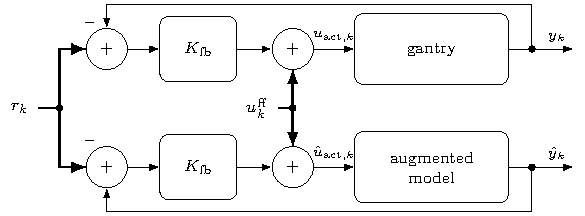
\includegraphics[width=\columnwidth]{closed_loop_same_reference.pdf}
 \caption{
Recorded system loop (top) and augmented model loop (bottom),
both using the same feedback controller, reference $r_k$
and feedforward $u_k^{\mathrm{ff}}$.
The model output is calculated before the input updates
the model state.
}
 \label{fig:aug_closed_loop}
\end{figure}

\subsection{Identification}\label{sec:aug_closed_loop}
\ifdraft
\begin{itemize}
\item $\theta_{\mathrm{base}}$ is estimated jointly with network and encoder, as in 2026 Eq.~(22); Kessels trains only the network weights (Eq.~(5.12))
\item Training coordinates $\beta$, zero at $\theta^0_{\mathrm{base}}$: nine combinations logarithmic, $m_\Delta$ through \eqref{eq:mdelta_map}; every $\beta$ admissible, so no clamp or penalty (this work, D-229; adapted from Drenth Sec.~4.2)
\item Criterion \eqref{eq:aug_loss}: Eq.~(22) adapted by the loop of Section~\ref{sec:aug_loop} and the encoder of Section~\ref{sec:aug_encoder}; every window sample scored; controller fixed; a closed-loop fit can mask plant error (Section~VI)
\item The baseline/network split is not unique (2026 Sec.~5.2), so $\theta_{\mathrm{base}}$ is not interpretable in the sense of Section~I; Section~IV addresses this (unique to first order only?)
\item Adam, then an unbounded L-BFGS polish (adapted from Drenth Sec.~5.1); checkpoint with the lowest closed-loop free-run error over whole validation records; polish kept only if it lowers that error
\item Initialisation \eqref{eq:aug_init}: $\tilde x$ and $\hat y$ reproduce the baseline, $\bar x$ evolves through a live $g_{\mathrm{aug}}$ (2026 Eq.~(29)); adapted from Sec.~5.4.3 (random added-state rows, no linear bypass); the model is named in Section~\ref{sec:setup}, not here
\end{itemize}
\fi
The network, encoder and $\theta_{\mathrm{base}}$ are jointly estimated, 
as in~\cite[Eq.~(22)]{hoekstra2026lfr}.
The optimiser updates $\theta_{\mathrm{base}}$ using $\beta\in\R^{10}$.
The nine positive parameter combinations are
$\theta_{\mathrm{base},j}=\theta^0_{\mathrm{base},j}\,e^{\beta_j}$,
while $m_\Delta$ can be positive or negative and is bounded
by \eqref{eq:lfr_admissibility}:
\begin{equation}
  m_\Delta=\rho\,\frac{2}{L_b}\sqrt{m_\Sigma J_{\mathrm{eff}}}\,
  \tanh\bigl(\eta_0+s\,\beta_\Delta\bigr),
  \label{eq:mdelta_map}
\end{equation}
where $\beta_\Delta$ determines $m_\Delta$ and
$\rho\in(0,1)$ provides a safety margin.
We choose the offset $\eta_0$ and scale $s$ so that
$\beta=0$ gives $m_\Delta=m_{\Delta,0}$ and
$\partial m_\Delta/\partial\beta_\Delta=m_{\Delta,0}$.
This matches the logarithmic parameters, where
$\partial\theta_{\mathrm{base},j}/\partial\beta_j
=\theta^0_{\mathrm{base},j}$ at $\beta=0$
(Appendix~\ref{app:lfr-wellposed}).
The initial value must satisfy
$\lvert m_{\Delta,0}\rvert<\rho(2/L_b)\sqrt{m_{\Sigma,0}J_{\mathrm{eff},0}}$.
The bound in \eqref{eq:lfr_admissibility} holds for
every $\beta$, therefore no clamping or penalty is needed.
\\
The parameters
$\vartheta=(\beta,\theta_{\mathrm{aug}},\theta_{\mathrm{enc}})$
are trained to minimise the normalised output error of the
closed-loop simulation, with the
controller fixed. We adapt this from~\cite[Eq.~(22)]{hoekstra2026lfr}, 
adapted for the closed loop of Section~\ref{sec:aug_loop} and the
encoder of Section~\ref{sec:aug_encoder}:
\begin{equation}
\begin{aligned}
 &\min_{\vartheta}\;V(\vartheta)=\frac{1}{|\mathcal W|\,n_f\,n_y}
 \sum_{\tau\in\mathcal W}\sum_{k=\tau}^{\tau+n_f-1}
 \norm{y^{\mathrm n}_{k}-\hat y^{\mathrm n}_{k|\tau}}_2^2\quad\text{s.t.}\\
 &\tilde x^{\mathrm n}_{k+1|\tau}
  =f^{\mathrm n}_{\mathrm{base}}\bigl(\theta_{\mathrm{base}}(\beta),
   \tilde x^{\mathrm n}_{k|\tau},\hat u^{\mathrm n}_{k|\tau}\bigr)
  +f^{\mathrm n}_{\mathrm{aug}}\bigl(\theta_{\mathrm{aug}},
   \hat x^{\mathrm n}_{k|\tau},\hat u^{\mathrm n}_{k|\tau}\bigr),\\
 &\bar x_{k+1|\tau}=g^{\mathrm n}_{\mathrm{aug}}\bigl(\theta_{\mathrm{aug}},
   \hat x^{\mathrm n}_{k|\tau},\hat u^{\mathrm n}_{k|\tau}\bigr),\\
 &\hat x^{\mathrm n}_{\tau|\tau}=\psi(\theta_{\mathrm{enc}},\chi_\tau),\quad
  \hat y^{\mathrm n}_{k|\tau},\,\hat u^{\mathrm n}_{k|\tau}\text{ from \eqref{eq:aug_cl_step}},
\end{aligned}
\label{eq:aug_loss}
\end{equation}
for $\tau\le k<\tau+n_f$, where each training window starts at a sample
$\tau\in\mathcal W$ and has length $n_f$, $n_y=3$, and
$\theta_{\mathrm{base}}(\beta)$ gives the baseline parameters.
\todo{might have to move to discussion if i dont add it. Since the controller corrects part of the output error,
it can hide errors in the plant model.
We therefore also test the model with a different controller
in Section~\ref{sec:results}.}
\\
The baseline parameters and the neural network can both correct the same 
model errors, making the optimal parameter values  
not unique~\cite[Sec.~5.2]{hoekstra2026lfr}.
Without enforcing uniqueness the estimated $\theta_{\mathrm{base}}$ is not 
interpretable as defined in Section~\ref{sec:intro}.
Section~\ref{sec:obc} extends the identification to separate what the 
neural network can learn from the baseline parameters.
\todo{Missing: Section~\ref{sec:obc} makes the 
network orthogonal to the linearised baseline sensitivity at
fixed tuples, so the split is unique only to first order 
around $\beta_{\mathrm{lin}}$, not a unique 
minimiser of \eqref{eq:aug_loss}. Candidate: 
once Section~\ref{sec:obc} states that local 
result, write ``so that the split is unique to first
order'' with a pointer to it 
(basis: \texttt{04\_obc.tex} \eqref{eq:obc_coef}; 
math check 2026-10-13, F1).}
\\
For training we minimise $V$ with Adam on minibatches of windows, and 
the gradient is calculated over the full window.
We then polish with L-BFGS on a fixed set of windows.
This is adapted from the Adam and L-BFGS-B sequence of Drenth
et al.~\cite[Sec.~5.1]{drenth2025lpvlfr}.
Because every $\beta$ satisfies \eqref{eq:lfr_admissibility}, 
unconstrained L-BFGS works without a bound.
During the optimization with Adam the parameters with the lowest validation 
error are kept.
The error is the RMS output error in meters for each complete validation record, 
simulated in closed loop with the initial state estimated
once by the encoder and $x^c=0$.
We only keep the polish if it lowers the validation error.
\todo{Current runs (\texttt{FINAL-RUN-FIXES.md} item~2): the 2026-10-11 runs also reject the polish if \texttt{combo\_err}, the error of the ten combinations against the true parameters, rises by more than 0.1\,\%. This uses the simulated truth; the final runs accept on the validation error alone. \texttt{param\_loss} is zero in all thesis runs (\texttt{param\_prior} off).}
\\
We start training with the augmented model giving the same
output as the baseline model from the same initial state, as required
by~\cite[Eq.~(29)]{hoekstra2026lfr}. \revnote{I use the encoder 
for my augmented model, so i state: model from the same initial state. 
But i could leave it out.}
Therefore we zero the physical rows of $\phi_{\mathrm{aug}}$ its output layer, 
and the added-state rows are kept random:
\begin{equation}
\begin{aligned}
 &\text{baseline:} &&\beta=0,\\
 &\text{network:}  &&W^{\tilde x}_L=0,\quad b_L=0,\quad W^{\bar x}_L\sim\mathcal U(-c,c),\\
 &\text{encoder:}  &&\theta^{b,0}_{\mathrm{enc}}\text{ from \eqref{eq:aug_enc_fit}},\\
 &                 &&W^a\sim\mathcal U(-a,a),\quad \tilde W^{\bar x}_L=0,\quad \tilde b^{\bar x}_L=0,\\
 &                 &&c=1/\sqrt{n_h},\quad a=\sqrt{6/(n_{\bar x}+6(n+1))},
\end{aligned}
 \label{eq:aug_init}
\end{equation}
where $W_L$ and $b_L$ are the output layer weights and bias of
$\phi_{\mathrm{aug}}$, with rows $W^{\tilde x}_L$ for
$f^{\mathrm n}_{\mathrm{aug}}$ and $W^{\bar x}_L$ for
$g^{\mathrm n}_{\mathrm{aug}}$.
The number of neurons per hidden layer $n_h$, 
$\tilde W^{\bar x}_L$ and $\tilde b^{\bar x}_L$
are the added-state rows of the output layer weights and bias of $\tilde\psi$.
We initialise $W^{\bar x}_L$ and the hidden layers of $\phi_{\mathrm{aug}}$
from $\mathcal U(-1/\sqrt{m},1/\sqrt{m})$,
where $m$ is the input size of the layer.
We use Xavier initialisation for $W^a$,
following~\cite[Eq.~(31)]{hoekstra2026lfr}.
We choose the uniform distribution with gain one,
giving $a=\sqrt{6/(n_{\bar x}+6(n+1))}$.
At the start of training, $\theta_{\mathrm{base}}=\theta^0_{\mathrm{base}}$
and $f^{\mathrm n}_{\mathrm{aug}}=0$.
The augmented model and baseline model give the same $\tilde x$ and $\hat y$, 
given they start from the same physical state.
The added states $\bar x$ are still updated by
$g^{\mathrm n}_{\mathrm{aug}}$, as in~\cite[Eq.~(29)]{hoekstra2026lfr}.
\\
\revnote{The current results start $W^b$ from the model-based
reconstructability map~\cite[Eqs.~(15) to (17)]{hoekstra2026encoder} of the
baseline linearised at rest at $Y=0$, and the whole output layer of
$\tilde\psi$ at zero. The final runs will start the physical encoder rows from
$\theta^{b,0}_{\mathrm{enc}}$ of \eqref{eq:aug_enc_fit} as described here.}
\revnote{The current results start with the whole output
layer of $\phi_{\mathrm{aug}}$ at zero, so $g_{\mathrm{aug}}=0$ and the added
states are zero after the first step. The final runs will use live
$g_{\mathrm{aug}}$ as described here.}
\todo{Current runs: the 2026-10-11 runs (R1 to R7) set the whole output layer of $\phi_{\mathrm{aug}}$ to zero (\texttt{G\_INIT} zero, D-240), as the authors' public code does (D-237), so $g^{\mathrm n}_{\mathrm{aug}}=0$ and $\bar x$ is zero after the first step. The final runs use \eqref{eq:aug_init} (D-248, \texttt{FINAL-RUN-FIXES.md} item~6).}

\subsection{Added-state initialisation}\label{sec:aug_ps2}
\ifdraft
\begin{itemize}
\item Problem: the start \eqref{eq:aug_init} gives $\tilde x$ a model ($f_{\mathrm{base}}$, $W^b$, output) and $\bar x$ none (random $W^a$, random added-state rows of $\phi_{\mathrm{aug}}$); $V$ scores only the output and $f_{\mathrm{aug}}$ can lower the same error statically, so training can leave the omitted dynamics out of $\bar x$ (Venkatraman Sec.~2.1; Section~VI tests it)
\item PS is this work's, adapted from two-stage regression (Hefny Sec.~2) and its use before BPTT (Downey Sec.~4.2); it gives $\bar x$ a start from data, as $W^b$ gives $\tilde x$ one from the baseline
\item S1: a decoder on $\psi_a$ predicts the current model's residual over $\tau+1$ to $\tau+H$; the minimiser is the conditional mean, so $\bar x_{\tau|\tau}$ becomes a predictive state; trains $\theta_{\mathrm p}$, $\theta^a_{\mathrm{enc}}$ only, one update after every update of $V$
\item Stopping rule: $\nu$ on calibration windows ends S1 (plateau or cap) and decides whether S2 runs
\item S2: once, one-step regression of $g^{\mathrm n}_{\mathrm{aug}}$ on frozen encoder pairs with the recorded input, which equals the loop input when the encoder reproduces $y_{k_i}$; overlapping windows (?)
\item Hand-over: decoder discarded, \eqref{eq:aug_loss} continues from $\vartheta_{\mathrm{PS}}$; deployed model, criterion and selection unchanged; $\bar x$ latent; $\mathcal M_{\mathrm{PS}}$ named
\item The current runs differ in two points: $g_{\mathrm{aug}}$ starts at zero, and the S1 target starts at $\tau$ (?)
\end{itemize}
\fi

The physical states of the baseline are initialized with the 
data-based fit \eqref{eq:aug_enc_fit} and updated through
$f^{\mathrm n}_{\mathrm{base}}$, while the added-state rows $W^a$ are randomly initialized.
For the physical states their generalized coordinates $q_k$ are directly mapped to 
actuator positions, $\hat y_k=P^\top q_k$ in \eqref{eq:aug_transition}.
The added states are updated through the random added-state rows of $\phi_{\mathrm{aug}}$, 
without their initialization or initial updates being derived from the baseline or the data.
The output $\hat y_k=P^\top q_k$ contains no added state, and $\bar x_k$
enters $\tilde x_{k+1}$ only through $f^{\mathrm n}_{\mathrm{aug}}$ in
\eqref{eq:aug_loss}. This means that for the added states $V$ only updates their effect on 
the output through $f^{\mathrm n}_{\mathrm{aug}}$.
From \eqref{eq:aug_loss}, $V$ contains nothing that directly incentivises $\bar x$
to predict the resulting output error.
This gives $f^{\mathrm n}_{\mathrm{aug}}$ the capability to lower part of this error with 
$\tilde x$ and $\hat u$ alone.
Minimising $V$ can therefore reduce the error without capturing the missing
dynamics in $\bar x$. \todo{Section~\ref{sec:results} tests whether it does.}
This forms a sharp contrast between the physical and added states,
due to the physical states being able to directly map to the output, 
while also having a much better starting point.

\todo{Current runs: the 2026-10-11 runs (R1 to R7) start the whole output layer of $\phi_{\mathrm{aug}}$ at zero (\texttt{G\_INIT} zero, D-240), as the authors' public code does (D-237), so $g^{\mathrm n}_{\mathrm{aug}}=0$ and $\bar x$ is zero after the first step. In the final runs, the added-state rows of the network's final output layer are randomly initialized (D-248, \texttt{FINAL-RUN-FIXES.md} item~6); \eqref{eq:aug_init} in Section~\ref{sec:aug_closed_loop} then changes accordingly. PS with a live start is so far one seed with the ResNet variant ($4.0\times10^{-6}$~m against $1.0\times10^{-5}$~m for plain training).}

%\\

We therefore propose predictive-state (PS) initialisation, which is
a data-driven initialisation for the added states. 
Similar to $W^b$ after its initialisation is done, 
the parameters are optimized through \eqref{eq:aug_loss}.
PS is adapted from a two-stage regression of predictive-state
learning~\cite[Sec.~2]{hefny2015supervised}, and it makes use of initialisation
before backpropagation through time~\cite[Sec.~4.2]{downey2017psrnn}.
%\\

The first stage (S1) predicts the residual of the model, instead 
of \kw{features of future observations} as in~\cite{hefny2015supervised}.
The second stage (S2) trains the nonlinear state update
instead of a \kw{linear operator.}
\kw{We continue training $V$ during the first stage, while Downey et al.\ finish
their initialisation before starting BPTT~\cite[Sec.~4.2]{downey2017psrnn}.}
Fig.~\ref{fig:ps2_windows} shows which samples
are used for both stages.

\begin{figure}[t]
 \centering
 \resizebox{\columnwidth}{!}{% PS windows on one record (Section III-E), layout adapted from Hefny et al. 2015, Fig. 2.
% Matches model_augmentation/fit_systems/ps2_opening.py (_sample, _residual, _fit_map), D-250:
% S1: chi_tau = samples tau-n-1 .. tau-1, residual e_tau = tau .. tau+H-1 (H = n+1);
% S2: chi_{tau+1} = tau-n .. tau, recorded input u_tau.
\begin{tikzpicture}[
    >={Latex[length=1.8mm,width=1.3mm]},
    line width=0.5pt,
    smp/.style={draw, line width=0.5pt, minimum width=10.5mm, minimum height=5mm,
                inner sep=0pt, font=\scriptsize},
    blk/.style={draw, line width=0.6pt, rounded corners=1pt, fill=white,
                align=center, inner sep=2pt, minimum height=6mm, minimum width=9mm},
    lab/.style={font=\scriptsize, inner sep=1.5pt},
    hop/.style={preaction={draw=white, line width=2.4pt}},
  ]
  \def\w{1.05}   % sample pitch
  \def\h{0.525}  % half sample width
  \def\g{0.09}   % bracket inset, keeps adjacent windows visibly apart
  \def\yB{0.47}  % bracket height above and below the row
  \def\yS{1.25}  % S1 blocks
  \def\yA{-1.1}  % psi_a row
  \def\yG{-1.85} % g_aug row
  \def\xL{-0.85} % route of x-hat_tau
  \def\xV{6.45}  % loss blocks
  % sample row
  \foreach \i/\t in {0/{$\tau{-}n{-}1$}, 1/{$\tau{-}n$}, 2/{$\cdots$}, 3/{$\tau{-}1$},
                     4/{$\tau$}, 5/{$\cdots$}, 6/{$\tau{+}H{-}1$}}
    \node[smp] (s\i) at (\i*\w,0) {\t};
  \node[lab, anchor=west] at (6*\w+\h+0.05,0) {$(y_k,u_k)$};

  % S1 (top): encoder window chi_tau and residual target e_tau, disjoint
  \draw (-\h+\g,\yB-0.1) -- (-\h+\g,\yB) -- (3*\w+\h-\g,\yB) -- (3*\w+\h-\g,\yB-0.1);
  \node[lab, anchor=south west] at (-\h+\g,\yB) {$\chi_\tau$};
  \draw (4*\w-\h+\g,\yB-0.1) -- (4*\w-\h+\g,\yB) -- (6*\w+\h-\g,\yB) -- (6*\w+\h-\g,\yB-0.1);
  \node[lab, anchor=south west] at (4*\w-\h+\g,\yB) {$e_\tau$};
  \node[blk] (psi) at (1.5*\w,\yS) {$\psi$};
  \node[blk] (dec) at (4.4*\w,\yS) {$p$}; % decoder d -> p (Dirk 2026-10-22: d is a baseline parameter)
  \node[blk] (v1) at (\xV,\yS) {$\|{\cdot}\|_2^2$};
  \draw[->] (1.5*\w,\yB) -- (psi.south);
  \draw[->] (psi.east) -- (dec.west) node[midway, above, lab] {$\bar x_{\tau|\tau}$};
  \draw[->] (dec.east) -- (v1.west);
  \draw[->] (\xV,\yB) -- (v1.south);

  % S2 (bottom): window shifted by one sample (ends at tau), one-step map g_aug
  \draw (1*\w-\h+\g,-\yB+0.1) -- (1*\w-\h+\g,-\yB) -- (4*\w+\h-\g,-\yB) -- (4*\w+\h-\g,-\yB+0.1);
  \node[lab, anchor=north west] at (1*\w-\h+\g,-\yB) {$\chi_{\tau+1}$};
  \node[blk] (psia) at (2*\w,\yA) {$\psi_a$};
  \draw[->] (2*\w,-\yB) -- (psia.north);
  \node[blk] (v2) at (\xV,\yA) {$\|{\cdot}\|_2^2$};
  \draw[->] (psia.east) -- (v2.west) node[pos=0.25, above, lab] {$\bar x_{\tau+1|\tau+1}$};
  \node[blk] (g) at (4*\w,\yG) {$g^{\mathrm n}_{\mathrm{aug}}$};
  % recorded input of the first residual sample, crossing the S2 bracket and the psi_a line
  \draw[->, hop] (s4.south) -- (g.north) node[pos=0.33, left, lab] {$u^{\mathrm n}_\tau$};
  % encoded state at tau, from the top encoder around the left
  \draw[->] (psi.west) -- (\xL,\yS) -- (\xL,\yG) -- (g.west)
       node[pos=0.08, lab, anchor=south west] {$\hat x^{\mathrm n}_{\tau|\tau}$};
  \draw[->] (g.east) -| (v2.south);
  % stage tags beside each loss: what that loss trains
  \node[lab, anchor=west, align=left] at ($(v1.east)+(0.08,0)$)
       {S1: trains\\$\theta_{\mathrm p}$, $\theta^a_{\mathrm{enc}}$};
  \node[lab, anchor=west, align=left] at ($(v2.east)+(0.08,0)$)
       {S2: trains\\$\theta_{\mathrm{aug}}$};
\end{tikzpicture}
}
 \caption{Windows of PS on one record, layout adapted
 from~\cite[Fig.~2]{hefny2015supervised}. S1 (top): the encoder maps the
 window $\chi_\tau$ to $\hat x^{\mathrm n}_{\tau|\tau}$, and the decoder $d$ maps its added part
 $\bar x_{\tau|\tau}$ to the residuals $e_\tau$ of the next $H$ samples
 \eqref{eq:ps2_s1}. S2 (bottom): $g_{\mathrm{aug}}$ maps $\hat x^{\mathrm n}_{\tau|\tau}$ and the
 recorded $u_\tau$ to the added state encoded from the window shifted by one
 sample \eqref{eq:ps2_s2}.
 \todo{The figure shows the target from $\tau+1$ (\texttt{FINAL-RUN-FIXES.md} item~5). The 2026-10-11 runs start it at $\tau$, so the noise in $y_\tau$ enters both $\chi_\tau$ and $e_\tau$.}}
 \label{fig:ps2_windows}
\end{figure}

%\\
% Stage S1 trains the encoder's added-state outputs to predict the residual of
% the augmented model \eqref{eq:aug_transition} at the parameters $\vartheta$
% after the latest update of $V$.
Stage S1 trains the encoder's added-state outputs to predict the residual of
the augmented model \eqref{eq:aug_transition} using the model parameters $\vartheta$
from the latest $V$ update step.
Each update of $V$ is followed by one S1 update with its own Adam optimiser.
For the S1 update we select a minibatch $\mathcal B$ of samples $\tau$ from the training data.
The training data is divided into excitation classes (\todo{see section}), and for classes 
with at least three records one is left out of S1 and S2 to evaluate $\nu$ \eqref{eq:ps2_nu}.
The left out data is still used in $V$.
For each sample $\tau$, the encoder uses the last $n+1$
samples up to $\tau$, $\chi_\tau$, to estimate the initial state $\hat x^{\mathrm n}_{\tau|\tau}$.
From this state the augmented model is simulated in the closed loop of 
Section~\ref{sec:aug_loop}.
We calculate the residual from the next $H=n+1$ samples, from $\tau+1$ to $\tau+H$.
\revnote{The current results use a residual target starting at $\tau$, so the
encoder and target share sample $\tau$. The final runs will start the target
at $\tau+1$, as described here.}
The top of Fig.~\ref{fig:ps2_windows} shows the window $\chi_\tau$ and the
samples of the residual $e_\tau$.
We have chosen to use the same number of samples as the encoder window.
Then a temporary decoder $d$ with only the added states as inputs
$\bar x_{\tau|\tau}=\psi_a(\theta_{\mathrm{enc}},\chi_\tau)$
is used to predict this residual:
\begin{equation}
\begin{aligned}
 e_\tau&=\frac{1}{\sigma_e}\col\bigl(y^{\mathrm n}_{k}-\hat y^{\mathrm n}_{k|\tau}\bigr)_{k=\tau+1}^{\tau+H},\\
 d(\theta_{\mathrm p},\bar x)&=W_{\mathrm p,2}\tanh\bigl(W_{\mathrm p,1}\bar x+b_{\mathrm p,1}\bigr)+b_{\mathrm p,2},\\
 &\min_{\theta_{\mathrm p},\,\theta^a_{\mathrm{enc}}}\;
 \frac{1}{|\mathcal B|\,H\,n_y}\sum_{\tau\in\mathcal B}
 \norm{d\bigl(\theta_{\mathrm p},\psi_a(\theta_{\mathrm{enc}},\chi_\tau)\bigr)-e_\tau}_2^2,
\end{aligned}
\label{eq:ps2_s1}
\end{equation}
% where $\hat y^{\mathrm n}_{k|\tau}$ is the output of the loop of
% Section~\ref{sec:aug_loop} from $\hat x^{\mathrm n}_{\tau|\tau}$ at the current
% $\vartheta$, held fixed in the gradient, $\mathcal B$ a minibatch of window
% ends $\tau$, $\sigma_e$ the RMS of all residual entries over $\mathcal B$, and
% $d:\R^{n_{\bar x}}\to\R^{Hn_y}$ the decoder with parameters
% $\theta_{\mathrm p}=(W_{\mathrm p,1},b_{\mathrm p,1},W_{\mathrm p,2},b_{\mathrm p,2})$,
% $W_{\mathrm p,1}\in\R^{n_h\times n_{\bar x}}$ and
% $W_{\mathrm p,2}\in\R^{Hn_y\times n_h}$.
% $W_{\mathrm p,2}$ and $b_{\mathrm p,2}$ start at zero, so the decoder first
% predicts no residual.
% Only $\theta_{\mathrm p}$ and $\theta^a_{\mathrm{enc}}$ receive a gradient,
% and the rest of $\vartheta$ is left to $V$.
where $\hat y^{\mathrm n}_{k|\tau}$ is the output from the
closed-loop simulation of Section~\ref{sec:aug_loop},
starting at $\hat x^{\mathrm n}_{\tau|\tau}$.
This simulated output is kept fixed during
the S1 update.
$\mathcal B$ is the minibatch of samples $\tau$ and
$\sigma_e$ is the RMS of all residual values in $\mathcal B$.
The decoder $d:\R^{n_{\bar x}}\to\R^{Hn_y}$ has parameters
$\theta_{\mathrm p}=(W_{\mathrm p,1},b_{\mathrm p,1},
W_{\mathrm p,2},b_{\mathrm p,2})$, with
$W_{\mathrm p,1}\in\R^{n_h\times n_{\bar x}}$ and
$W_{\mathrm p,2}\in\R^{Hn_y\times n_h}$.
Both $W_{\mathrm p,2}$ and $b_{\mathrm p,2}$ are initially
set to zero, so that the decoder starts by predicting zero residual.
Only $\theta_{\mathrm p}$ and $\theta^a_{\mathrm{enc}}$
are updated by S1. 
The parameters of $\vartheta$, including $\theta^a_{\mathrm{enc}}$
are still trained through $V$.
\\
The expected squared error is minimised by
the conditional mean $\mathbb E[e_\tau\mid\chi_\tau]$.
The decoder only sees up to $\bar x_{\tau|\tau}$, not the full history $\chi_\tau$, 
this forces the encoder to use the added states to predict the future residual.
\todo{
Instead of using features of future observations 
as Hefny et al.~\cite[Sec.~2]{hefny2015supervised} for predictive-state learning, 
we use the model residual.
}
To avoid correlation between the history and future noise Hefny et al.\ separate
the past and future samples~\cite[Sec.~2]{hefny2015supervised}. 
We borrow this principle by having the residual start at $\tau+1$, so that there 
is no overlap between the samples used for the encoder and to calculate the residual.
\todo{
Venkatraman et al.\ use a similar approach by predicting
future observations from the internal states during
training~\ucite[Sec.~3]{venkatraman2017psd}.
}
For the PS implementation the decoder predicts the model residual and
is removed after S1.
\todo{Current runs (\texttt{FINAL-RUN-FIXES.md} item~5): the 2026-10-11 runs start the target at $\tau$ (\texttt{ps2\_opening.py}, \texttt{\_sample} and \texttt{\_residual}), so sample $\tau$ is both the last sample of $\chi_\tau$ and the first of $e_\tau$, and the noise in $y_\tau$ enters both sides of \eqref{eq:ps2_s1}.}
\todo{Missing: Hefny et al.\ model the noise as independent per sample (Fig.~1). Our measurement noise is low-pass and fed back by the controller, so disjoint windows remove the shared sample but not all correlation between $\chi_\tau$ and the noise in $e_\tau$. Candidate: one sentence here or in the Discussion (basis: D-238 noise model).}

To evaluate how well $\bar x_{\tau|\tau}$ performs at predicting the residual, a
fixed set $\mathcal C$ of windows from the held out data is used.
For this set the squared prediction error of the decoder
divided by the squared residual is computed,
\begin{equation}
 \nu=\frac{\sum_{\tau\in\mathcal C}\norm{d\bigl(\theta_{\mathrm p},\psi_a(\theta_{\mathrm{enc}},\chi_\tau)\bigr)-e_\tau}_2^2}
 {\sum_{\tau\in\mathcal C}\norm{e_\tau}_2^2}.
 \label{eq:ps2_nu}
\end{equation}
S1 is stopped when a maximum number of updates is reached or when $\nu$ stops improving, or at an early check when $\nu$ is above $\nu_{\max}$.
S2 starts only if $\nu$ is below a threshold $\nu_{\max}$, else the decoder is removed 
and training continues. In both cases the encoder changes from S1 are kept.
The threshold rule for S2 is given in Appendix~\ref{app:ps_stop}.
\todo{Missing: basis of the PS switch and stop rules (S1 plateau and cap, screen update and threshold, S2 plateau and cap, snapshot sizes, calibration split as the last record of each class with three or more records). Candidate: rows of the hyperparameter table in Section~\ref{sec:setup}, all HEURISTIC (\texttt{PS2Spec}; \texttt{PS2-METHOD.md} Sec.~5), noting that the S1 cap, not the plateau, ended S1 in every run so far.}


S1 has only trained the part of the encoder that initializes the 
added states $\bar x_{\tau|\tau}$, $g^{\mathrm n}_{\mathrm{aug}}$ 
is only updated by $V$. 
S2 trains the state update itself.
In S2 $g^{\mathrm n}_{\mathrm{aug}}$ is trained to predict the next
added state $\bar x_{k+1}$ from the full state $\hat x^{\mathrm n}_k$ and the input
$u^{\mathrm n}_k$.
For S2 samples $k_i$ from the training data are selected, 
except the same held-out records from S1 are left out.
For each sample the encoder estimates $\hat x^{\mathrm n}_{k_i|k_i}$ from
$\chi_{k_i}$ and $\bar x_{k_i+1|k_i+1}$ from the next window
$\chi_{k_i+1}$.
Fig.~\ref{fig:ps2_windows} shows an example with $k_i=\tau$.
The window $\chi_\tau$ at the top is used for $\hat x^{\mathrm n}_{k_i|k_i}$,
and the shifted window at the bottom is used for $\bar x_{k_i+1|k_i+1}$.
We calculate these pairs once after S1, this set $\mathcal P$ is kept fixed. 
\\
During S2 the model is not simulated in closed-loop and $V$ is paused.
We instead train $g^{\mathrm n}_{\mathrm{aug}}$ on
$\mathcal P$ using one-step regression with the recorded
actuator force $u^{\mathrm n}_{k_i}$ as input, and a separate Adam optimiser:
\begin{equation}
\begin{aligned}
 \mathcal P&=\bigl\{(\hat x^{\mathrm n}_{k_i|k_i},\,u^{\mathrm n}_{k_i},\,\bar x_{k_i+1|k_i+1})\bigr\}_{i=1}^{N_{\mathcal P}},\\
 \hat x^{\mathrm n}_{k_i|k_i}&=\psi(\theta_{\mathrm{enc}},\chi_{k_i}),\quad
 \bar x_{k_i+1|k_i+1}=\psi_a(\theta_{\mathrm{enc}},\chi_{k_i+1}),\\
 &\min_{\theta_{\mathrm{aug}}}\;
 \frac{\sum_{i\in\mathcal B_{\mathcal P}}\norm{g^{\mathrm n}_{\mathrm{aug}}\bigl(\theta_{\mathrm{aug}},\hat x^{\mathrm n}_{k_i|k_i},u^{\mathrm n}_{k_i}\bigr)-\bar x_{k_i+1|k_i+1}}_2^2}
 {\sum_{i\in\mathcal B_{\mathcal P}}\sum_{j=1}^{n_{\bar x}}\bigl(\bar x_{j,k_i+1|k_i+1}-m_j\bigr)^2},
\end{aligned}
\label{eq:ps2_s2}
\end{equation}
where $\theta_{\mathrm{enc}}$ is not updated during S2,
$\mathcal B_{\mathcal P}\subset\mathcal P$ is a minibatch,
$\bar x_{j,\cdot}$ is the $j$th added state and $m_j$
is the mean of $\bar x_{j,k_i+1|k_i+1}$ over $\mathcal B_{\mathcal P}$.
The cost is the fraction of the variance in the
next added states that is not explained by the prediction.
\\
The parameters with the lowest cost on the separate set of pairs 
from the held-out records are kept.
For S2 we use the recorded actuator force $u^{\mathrm n}_{k_i}$
applied to the system at $k_i$.
The encoder estimates $\bar x_{k_i+1|k_i+1}$ from
$\chi_{k_i+1}$, using the data up to $k_i+1$.
At the start of a window in \eqref{eq:aug_residual_loop}
$x^c=0$, resulting in the model input
\begin{equation*}
 \hat u_{\mathrm{act},k_i}=u_{\mathrm{act},k_i}+D_{\mathrm{fb}}\bigl(y_{k_i}-\hat y_{k_i|k_i}\bigr),
\end{equation*}

when the encoder reproduces $y_{k_i}$ this equals the recorded input, 
because at this sample only the controller feedthrough $D_{\mathrm{fb}}$
acts on the output error.
For S2 $g^{\mathrm n}_{\mathrm{aug}}$ is therefore trained with approximately
the input it receives at that sample in the closed-loop simulation of $V$.
S2 updates all parameters $\theta_{\mathrm{aug}}$ of $\phi_{\mathrm{aug}}$.
The cost only depends on the added-state rows, so the physical rows of $W_L$ and $b_L$
are not changed.
The hidden layers of $\phi_{\mathrm{aug}}$ are shared by
$f^{\mathrm n}_{\mathrm{aug}}$ and $g^{\mathrm n}_{\mathrm{aug}}$, so S2 also
updates $f^{\mathrm n}_{\mathrm{aug}}$.
\todo{The encoder windows at $k_i$ and $k_i+1$ share measurement samples, so noise enters both sides of the S2 regression. Hefny et al.\ discuss how correlated noise can bias such a fit~\cite[Sec.~2]{hefny2015supervised}. We do not correct for this effect in S2.}
When S2 is completed the optimization continues minimizing
\eqref{eq:aug_loss}
\begin{equation}
 \vartheta_{\mathrm{PS}}
 =\bigl(\beta^{(i_1)},\,\theta^{\mathrm{S2}}_{\mathrm{aug}},\,\theta^{(i_1)}_{\mathrm{enc}}\bigr),
 \label{eq:ps2_handover}
\end{equation}
followed by the L-BFGS polish and selection of Section~\ref{sec:aug_closed_loop}.
Here $\beta^{(i_1)}$ and $\theta^{(i_1)}_{\mathrm{enc}}$ are the parameters
after S1 and $\theta^{\mathrm{S2}}_{\mathrm{aug}}$ contains the parameters
after S2. When S2 is skipped, $\vartheta_{\mathrm{PS}}$ contains the
parameters at the end of S1.
\\
PS has only changed the starting point of minimising $V$ 
with its initialization phases, not what is being minimized.
The models with and without PS have the same number of parameters, 
since the decoder is removed.

% Page budget: 1.55 pages | Owns: negation, OBC derivation, additional-state scope, implementation, and true-parameter condition.
% WRITING GUIDE
% Purpose: Explain negation, derive the final state-level orthogonal-by-construction map, and delimit its interpretability guarantee.
% Sources: README "Source map per subsection", rows IV-A to IV-D; mandatory papers and the reference gate as in the README.
% Research-plan anchor: Preserve Aspect 3's goal of protecting physical interpretability; state clearly how the final construction differs from the proposed regularisation.
% Current decisions: Reduced identifiable coordinates, data-derived reference tuples, a tangent-only one-step physical-state projection, per-epoch refresh, and no affine comparison arm.
% Choices to justify: Protected parameter coordinates, reference-set construction, projected rows, rank tolerance, exclusion of the affine offset, refresh frequency, and treatment of additional states.
% Cautions: docs/orthogonal-projection-plan.md describes an older soft-penalty route; one-step state orthogonality is not trajectory-output orthogonality or guaranteed true recovery.
% Planned figures: New geometric projection figure with a physical and additional-state partition inset; show the remaining uniqueness limitation as clearly as the protected direction.
% Section is finished when: The protected space, coordinate frame, gradient treatment, added-state scope, and true-recovery condition are explicit.
%
% MUST ESTABLISH (agreed with Dirk 2026-10-09, revised 2026-10-14 and 2026-10-15; step 2a of the
%   thesis-section skill). Section IV is about orthogonality and stays general: no data, band, sample-rate or
%   record statements (those are Section V and Results). Math first: every step a display. We use orthogonality
%   by construction, not regularisation: the penalty is not discussed; the 2025 regularisation paper is cited
%   only where its concepts are used (state-level stacking Eq. 9, parameter Jacobian Sec. 4 Eq. 15, simulated
%   states Sec. 3, per-epoch recomputation Sec. 3 Remark 2, offset column Eqs. 17, 18).
%  Opening (Dirk's text): non-unique pair; the network can represent what theta_base explains; orthogonality
%          defined in words; unique, not necessarily true; Gyorok IO linear-in-parameters, we extend to state
%          space nonlinear in its parameters. No roadmap. Added states NOT in the opening (they are in IV-B).
%  IV-A Orthogonal-by-construction parametrisation (Gyorok 2026, adopted), eq:obc_gyorok: theta_aux is the
%          least-squares fit of the network output by the regressor; that part is removed; the remainder is
%          orthogonal on the training data (Lemma 3); theta_aux exists for full column rank (Assumption 1, Eq.
%          6: identifiable baseline, weakly persistently exciting input); data-driven: holds on the data used,
%          depends on their distribution (Sec. 3.2, text after Eqs. 12, 13); uniqueness of theta_b shown under
%          Assumption 1 AND exact fit (Assumption 6, Sec. 4.2).
%  IV-B Extension to the gantry (this work; label sec:obc_map kept for the refs in Sections I and VI):
%       a. nonlinear in the parameters: Jacobian eq:obc_sens (2025 Eq. 15); columns = Y-dependent mass, damping,
%          stiffness forces; Gamma left out, it does not enter the estimate (D-254; supervisor revnote outside wip).
%       b. full column rank (Assumption 1) through the ten identifiable combinations: 14 raw parameters give four
%          structural null directions (Section II-C, D-190); beta map invertible (D-229); rank then needs only
%          excitation (2026 Eq. 6).
%       c. only positions measured: tuples eq:obc_tuples from the data (2026 Eq. 5; 2025 Sec. 3 simulates
%          instead; D-254); each with a successor (D-252, revnote); coefficient on the stack eq:obc_coef.
%       d. our definition of orthogonality eq:obc_orth, on the reference tuples at xbar = 0 (Lemma 3 adapted);
%          measured by the normalised inner product eq:obc_overlap: cos angle, c_j per parameter direction,
%          rho = max over ran Phi = ||Pi d|| / ||d|| (supervisor: orthogonality is measured by the inner product;
%          Dirk 2026-10-15). Section V says what it is applied to (D-246: corrected f_aug on held-out tuples,
%          eps in simulation, eval_overlap.py; c_j not computed yet).
%       e. closed-loop state update: eq:obc_corr, correction at every step, added states not corrected,
%          coefficient differentiated (2026 Eqs. 9, 10, 13).
%       f. identification of M_OBC in prose (no separate display; the cost does not change): eq:aug_loss with
%          the corrected row; theta_aux re-solved per evaluation; beta_lin per epoch (2025 Remark 2, Sec. 4);
%          rebuild after restore; polish revnotes (D-253, D-255).
%       g. what it guarantees: eq:obc_eps, eq:obc_recovery (adapted from 2026 Thm. 7 without Assumption 6);
%          true iff Phi^T eps = 0 (excitation, Remark 5); Kessels' negation not prevented; one-step surrogate.
%  Removed 2026-10-15: the old problem paragraph (eq:obc_nonunique), eq:obc_problem and the separate
%          identification subsection (sec:obc_ident), the projection figure, the per-phase details, the
%          pseudoinverse "+" notation ((Phi^T Phi)^{-1} Phi^T throughout, as in Gyorok 2026 Eq. 8; Dirk).
%
% DRAFT NOTES (revision 2026-10-09 of the cycle-17 draft)
% NOTATION (Dirk, 2026-10-15): as Gyorok, lower case per sample/tuple, upper case stacked over the data; no bold.
%   Per tuple varphi(beta_lin, x, u) (6x10), stack Phi (6N x 10), column Phi_j; network f_aug, stack F_aug; baseline
%   stack F_base; next states X_+. The stacked one-step discrepancy is Xi (Gyorok's Delta clashes with Delta(Y),
%   m_Delta, beta_Delta; eps clashes with the Section III output error eps_{k|tau}); label eq:obc_eps kept for refs.
%   Earlier note (superseded): A bar marks the added state (Section III), so the expansion point is xi_lin. Plain J
%   clashes with the inertias, so the sensitivity is Phi (Gyorok's letter). The correction is f^n_obc.
% SOURCE CONFLICTS: D-190 Why records the supervisors' condition as non-overlap with the baseline OUTPUT (an
%   affine [J c] range); D-192 makes the offset diagnostic only and gives no reason; D-186 (2026-09-10, written
%   for the trajectory basis) gives reasons 1 and 2. The draft states those reasons; the question is a todo.
% LEFT OUT: rank tolerance and rank-loss fallback; D-194 forward sensitivity and D-195 hoist (how the code
%   evaluates the same model); SVD solve; D-232 noisy-velocity check; pointwise no-go and Coulomb argument
%   (Discussion); overlap cosines (todo); the affine arm (not in the THESIS-RESULTS campaign).
% MOVED to other sections (not edited here): the fourth-order stencil basis (gain error below 0.2 percent
%   against about 2.2 percent for second order at 230 Hz, 4 kHz; obc-gantry-one-step-implementation-plan.tex
%   after eq. reference-reconstruction) to the Section V basis column; "the records are not designed for the
%   condition" and the detuned-start comparison to Section V and Results.
% STALE LINES in other sections (not edited): 06_results.tex line 40 cites eq:obc_overlap and rho_f, no longer
%   defined; 06_results.tex line 45 and 05_setup.tex line 52 quote the affine arm; 07_discussion.tex uses
%   J^T Delta* (now Phi^T eps, eq:obc_eps); 08_conclusion.tex line 19 "prevents local tangent overlap" uses
%   wording D-186 Ruled out (1) bars.
% CODE CONFIRMED (cycle 17, checker): obc_gantry.py build_reference_set, make_basis_builder,
%   GantryOBCCorrection.forward; obc.py OBCBasis.coefficient, OBCLifecycle.maybe_refresh; interconnect.py loss,
%   forward, _sync_prediction_state_for_validation; ps2_opening.py _residual; blocks.py transition_from_free.
\section{Interpretability by Orthogonal Construction}\label{sec:obc}
\ifdraft
\begin{itemize}
\item Goal from Section~III: an estimate of $\theta_{\mathrm{base}}$ that is unique under stated conditions; names IV-A and IV-B (style profile)
\item Contribution: the extension Gy\"or\"ok 2026 Sec.~6 leaves open: a state-space baseline without full-state measurement, here nonlinear in its parameters and identified in closed loop (this work)
\end{itemize}
\fi
\changelegend

The parameter pair $(\theta_{\mathrm{base}},\theta_{\mathrm{aug}})$
minimising the loss function of Section~\ref{sec:aug_closed_loop} can be non-unique:
different pairs can give the same fit~\cite[Sec.~3.1]{gyorok2026obc}.
Meaning that the rigid-body dynamics that the baseline parameters 
$\theta_{\mathrm{base}}$ are able to explain from the data, can instead be represented by 
a neural network correction.
To prevent the neural network from correcting what $\theta_{\mathrm{base}}$ 
can represent we introduce orthogonality by construction~\cite{gyorok2026obc}.
Orthogonality here is defined as the neural network correction to the
physical states having no component in the directions in which a change of
$\theta_{\mathrm{base}}$ is able to change the next state predicted by the baseline.
This gives us a unique estimate of $\theta_{\mathrm{base}}$ up to first order,
but it does not guarantee recovering the true baseline parameters.
\\
Gy\"or\"ok et al.\ have constructed this for input-output baseline models that
are linear in their parameters~\cite{gyorok2026obc}.
We extend this to state-space models nonlinear in their parameters,
specifically for our gantry system.
% RESTRUCTURE (2026-10-20, Dirk): roadmap, as in Sections III and IV.
\kwtwo{In this section, we first give the orthogonal-by-construction
parametrisation of Gy\"or\"ok et al.\ (Section~\ref{sec:obc_construction}),
then extend it to the gantry (Section~\ref{sec:obc_map}), state how the
augmented model is identified with it and when the true parameters are
recovered (Section~\ref{sec:obc_ident}), and finally how orthogonality is
measured (Section~\ref{sec:obc_measures}).}
\subsection{Orthogonal-by-construction parametrisation}\label{sec:obc_construction}
\ifdraft
\begin{itemize}
\item Gy\"or\"ok's construction as adopted: baseline linear in its parameters, regressor at measured input-output data (past outputs, past and current inputs), stacked over the training data; lower case per sample, upper case stacked (2026 Eqs.~(1), (2), (5))
\item $\theta_{\mathrm{aux}}$ is the least-squares fit of the network output by the regressor; its fitted part is removed and the remainder is orthogonal to $\Phi$ on the training data (2026 Eqs.~(8) to (11), Lemma~3)
\item $\theta_{\mathrm{aux}}$ exists for full column rank of $\Phi$: identifiable baseline, weakly persistently exciting input (2026 Eqs.~(6), (7), Assumption~1)
\item Data-driven: orthogonality holds on the data used, the projection depends on their distribution; any fixed set may be used, the analysis uses the whole training set (2026 Sec.~3.2, text after Eqs.~(12), (13))
\item Uniqueness of $\hat\theta_{\mathrm b}$ shown under Assumption~1 and exact reproduction of the noise-free dynamics on the same training data (2026 Sec.~4.2, Assumption~6)
\end{itemize}
\fi
For a baseline linear in its parameters,
$\hat y_k=\varphi(x_k)\theta_{\mathrm b}$,
changing $\theta_{\mathrm b}$ changes the model output $\hat y_k$
by a linear combination of the columns of the
regressor $\varphi(x_k)$~\cite[Eqs.~(2), (39)]{gyorok2026obc}.
Gy\"or\"ok et al.\ subtract from the neural network output
its least-squares fit by the stacked
regressor~\cite[Eqs.~(8), (9), (11), Lemma~3]{gyorok2026obc}:
\begin{equation}
\begin{aligned}
 \hat Y&=\Phi\theta_{\mathrm b}+\tilde F^{\mathrm{ANN}},\\
 \tilde F^{\mathrm{ANN}}&=F^{\mathrm{ANN}}-\Phi\theta_{\mathrm{aux}},\\
 \theta_{\mathrm{aux}}&=\bigl(\Phi^\top\Phi\bigr)^{-1}\Phi^\top F^{\mathrm{ANN}},\\
 0&=\Phi^\top\tilde F^{\mathrm{ANN}},
\end{aligned}
\label{eq:obc_gyorok}
\end{equation}
where $x_k$ is the vector of past measured outputs and past and current
inputs~\cite[Eq.~(1)]{gyorok2026obc}, $\hat Y$ stacks the
predicted outputs over the training data, $\Phi$ is the stacked
regressor, $F^{\mathrm{ANN}}$ stacks the parallel network
outputs~\cite[Eq.~(5)]{gyorok2026obc} and $\tilde F^{\mathrm{ANN}}$ is the
projected network output~\cite[Eqs.~(9), (10)]{gyorok2026obc}.
\\
The projected network output $\tilde F^{\mathrm{ANN}}$ is
orthogonal to the regressor~\cite[Lemma~3]{gyorok2026obc}.
Calculating $\theta_{\mathrm{aux}}$ requires
$(\Phi^\top\Phi)^{-1}$, which exists only if $\Phi$ has
full column rank~\cite[Assumption~1]{gyorok2026obc}.
Therefore different values of $\theta_{\mathrm b}$ are unable 
to give the same stacked prediction on the training data. 
Gy\"or\"ok et al.\ call an input with this property persistently
exciting~\cite[Eq.~(6), Sec.~4.3]{gyorok2026obc}.
This also requires an identifiable baseline, where different
values of $\theta_{\mathrm b}$ give different functions
$\varphi(\cdot)\theta_{\mathrm b}$.
\subsection{Extension to the gantry}\label{sec:obc_map}
\ifdraft
\begin{itemize}
\item Three differences, each changing one element of \eqref{eq:obc_gyorok}: regressor, data, prediction (this work)
\item Regressor: Jacobian of the normalised transition in $\beta$ at $\beta_{\mathrm{lin}}$, since the baseline is nonlinear through $M(Y)^{-1}$; $\beta$ because only the ten combinations are identifiable (adapted from Gy\"or\"ok 2025 Sec.~4, Eq.~(15); 2026 Assumption~1; Section~II-C; D-190, D-229); offset column $\Gamma$ included (D-257)
\item Data: reference tuples reconstructed from the measured positions, regressor at the data as in 2026 Eq.~(5) rather than at a simulated baseline (2025 Sec.~3); each with a successor; built once before training (D-252, D-254)
\item Projection on the stacked tuples, with the orthogonality of the section opening as its last line; holds for the stack at $\bar x=0$ (adapted from 2026 Eqs.~(8) to (11), Lemma~3)
\item Prediction: the correction at every step of the closed-loop state update, physical rows only; coefficient differentiated (2026 Eqs.~(9), (10), (13); added states this work)
\end{itemize}
\fi
Our baseline violates three requirements of the projection in
\eqref{eq:obc_gyorok}.
\chg{Its}{\kwtwo{First, its}} state update is nonlinear in the parameters, because
the next state update depends on $M(Y)^{-1}$ in \eqref{eq:base_ss},
violating the linear requirement for the regressor.
Instead of the regressor the Jacobian of the baseline state update is taken 
with respect to $\beta$,
as in the orthogonal regularisation method of
Gy\"or\"ok et al.~\cite[Sec.~4, Eq.~(15)]{gyorok2025l4dc}.
Like the regressor, the stacked Jacobian must have full column rank.
This requires identifiable parameters, which is why we use $\beta$.
The Jacobian is taken at a linearisation point $\beta_{\mathrm{lin}}$ as
\begin{equation}
 \varphi(\beta_{\mathrm{lin}},\tilde x^{\mathrm n},u^{\mathrm n})
 =\left.\frac{\partial f^{\mathrm n}_{\mathrm{base}}\bigl(\theta_{\mathrm{base}}(\beta),\tilde x^{\mathrm n},u^{\mathrm n}\bigr)}
   {\partial\beta}\right|_{\beta=\beta_{\mathrm{lin}}},
\label{eq:obc_sens}
\end{equation}
where $\beta_{\mathrm{lin}}\in\R^{10}$ and
$\varphi:\R^{10}\times\R^6\times\R^3\to\R^{6\times10}$.
\kw{The linearisation also leaves an offset that does not depend on
$\beta$~\cite[Eq.~(16)]{gyorok2025l4dc}:}
\begin{equation}
\begin{aligned}
 f^{\mathrm n}_{\mathrm{base}}\bigl(\theta_{\mathrm{base}}(\beta),\tilde x^{\mathrm n},u^{\mathrm n}\bigr)
 &\approx\varphi\,\beta+\gamma,\\
 \gamma
 &=f^{\mathrm n}_{\mathrm{base}}\bigl(\theta_{\mathrm{base}}(\beta_{\mathrm{lin}}),\tilde x^{\mathrm n},u^{\mathrm n}\bigr)
  -\varphi\,\beta_{\mathrm{lin}},
\end{aligned}
\label{eq:obc_offset}
\end{equation}
\kw{where $\gamma:\R^{10}\times\R^6\times\R^3\to\R^6$, so that
$\varphi\beta_{\mathrm{lin}}+\gamma$ is the next state predicted by the
baseline at $\beta_{\mathrm{lin}}$.
Gy\"or\"ok et al.\ add this offset as an extra column to the Jacobian, to
include all components of the baseline model in the
orthogonality~\cite[Eq.~(18)]{gyorok2025l4dc}.
We include it as well, so the neural network has no component along the
stacked next states predicted by the baseline.}
% RESTRUCTURE (2026-10-19, Maarten mail): moved below eq:obc_recovery, which
%   it used before its definition.
\delmv[M-mail]{V-C}{The offset does not change the first-order estimate \eqref{eq:obc_recovery}.}
\chg[M-mail]{\kw{It}}{\kwtwo{The offset}} \kw{does not fully prevent negation~\cite[Sec.~5.3.1.3]{kessels2025ai}, where
the neural network cancels part of the baseline response, because only the
part of the network along the stacked baseline response is excluded.}
% \\
% \revnote{Orthogonality here is to the stacked Jacobian and offset
% $\Phi_\Gamma$ on the tuples (Gy\"or\"ok et al.\ 2026, Lemma~3, with the
% regressor taken as $[\varphi\ \gamma]$, the offset as in Gy\"or\"ok et al.\
% 2025, Eq.~(18)). To first order the estimate of $\beta$ does not depend on
% the network, with or without $\Gamma$; not shown for the nonlinear
% closed-loop optimum. The current results are without $\Gamma$; the final
% % runs include it.}
% \\

\chg{The}{\kwtwo{Second, the}} Jacobian also depends on the state, while the regressor of
Gy\"or\"ok et al.\ uses only measured inputs and
outputs~\cite[Eqs.~(1), (2)]{gyorok2026obc}.
Since only the positions are measured, we evaluate the Jacobian at these
positions with the velocities reconstructed from them:
\begin{equation}
\begin{aligned}
 \tilde x_i&=\col(q_i,\dot q_i),\qquad q_i=P^{-\top}y_i,\\
 \dot q_i&=\frac{-q_{i+2}+8q_{i+1}-8q_{i-1}+q_{i-2}}{12\,T_s},
\end{aligned}
\label{eq:obc_tuples}
\end{equation}
where $y_i$ is the measured actuator position at sample $i$.
Each tuple $(\tilde x_i,\bar x_i,u_i)$ uses the recorded actuator 
force $u_i$ and $\bar x_i=0$,
with the physical state and input normalised to
$\tilde x^{\mathrm n}_i$ and $u^{\mathrm n}_i$
using \eqref{eq:aug_norm}.
The tuples are calculated once before training, using all samples for which
\eqref{eq:obc_tuples} can be calculated at $i$ and at the next sample $i+1$.
\\
Stacking the Jacobian, \kw{the offset} and the network output over the tuples, the projection
of \eqref{eq:obc_gyorok} becomes
\begin{equation}
\begin{aligned}
 \Phi_\Gamma
 &=\col\bigl([\varphi\ \ \gamma](\beta_{\mathrm{lin}},\tilde x^{\mathrm n}_i,u^{\mathrm n}_i)\bigr)_{i\in\mathcal I},\\
 F^{\mathrm n}_{\mathrm{aug}}(\theta_{\mathrm{aug}})
 &=\col\bigl(f^{\mathrm n}_{\mathrm{aug}}(\theta_{\mathrm{aug}},\col(\tilde x^{\mathrm n}_i,0),u^{\mathrm n}_i)\bigr)_{i\in\mathcal I},\\
 \theta_{\mathrm{aux}}(\theta_{\mathrm{aug}})
 &=\bigl(\Phi_\Gamma^\top\Phi_\Gamma\bigr)^{-1}\Phi_\Gamma^\top F^{\mathrm n}_{\mathrm{aug}}(\theta_{\mathrm{aug}}),\\
 \tilde F^{\mathrm n}_{\mathrm{aug}}(\theta_{\mathrm{aug}})
 &=F^{\mathrm n}_{\mathrm{aug}}(\theta_{\mathrm{aug}})-\Phi_\Gamma\,\theta_{\mathrm{aux}}(\theta_{\mathrm{aug}}),\\
 0&=\Phi_\Gamma^{\top}\tilde F^{\mathrm n}_{\mathrm{aug}}(\theta_{\mathrm{aug}}),
\end{aligned}
\label{eq:obc_coef}
\end{equation}
where $\mathcal I$ is the set of tuples, $N=|\mathcal I|$,
\kw{$\Phi_\Gamma=[\Phi\ \Gamma]\in\R^{6N\times11}$ stacks $\varphi$ and $\gamma$}
evaluated at $\beta_{\mathrm{lin}}$,
$F^{\mathrm n}_{\mathrm{aug}},\tilde F^{\mathrm n}_{\mathrm{aug}}\in\R^{6N}$
and $\theta_{\mathrm{aux}}\in\R^{\kw{11}}$.
The projected network output $\tilde F^{\mathrm n}_{\mathrm{aug}}$ therefore
has no component along any column of $\kw{\Phi_\Gamma}$, which satisfies our orthogonality
definition at the start of this section.
This holds for the stacked tuples at $\bar x=0$, not for each tuple separately.
\\
\chg{We}{\kwtwo{Third, we}} use a state-space model predicting the next state instead of the output.
The fitted part is removed from the neural network correction of the
physical state at every step in the closed-loop simulation.
At each step, we subtract the Jacobian \kw{and offset} multiplied by
$\theta_{\mathrm{aux}}$ from the network correction,
evaluated at the current state and input.
Gy\"or\"ok et al.\ apply the same correction to the predicted
output~\cite[Eqs.~(9), (13)]{gyorok2026obc}.
The baseline has no added states, so its Jacobian \kw{and offset are} zero
in the added-state rows and $g^{\mathrm n}_{\mathrm{aug}}$
is orthogonal to it by definition.
We therefore only correct the physical rows:
% Only the physical rows are corrected, because the baseline has no added-state
% update:
\begin{equation}
\begin{aligned}
 f^{\mathrm n}_{\mathrm{obc}}(\theta_{\mathrm{aug}},\tilde x^{\mathrm n},u^{\mathrm n})
 &=[\varphi\ \ \gamma](\beta_{\mathrm{lin}},\tilde x^{\mathrm n},u^{\mathrm n})\,
  \theta_{\mathrm{aux}}(\theta_{\mathrm{aug}}),\\
 \tilde x^{\mathrm n}_{k+1|\tau}
 &=f^{\mathrm n}_{\mathrm{base}}+f^{\mathrm n}_{\mathrm{aug}}-f^{\mathrm n}_{\mathrm{obc}},\\
 \bar x_{k+1|\tau}&=g^{\mathrm n}_{\mathrm{aug}},
\end{aligned}
\label{eq:obc_corr}
\end{equation}

where
$f^{\mathrm n}_{\mathrm{obc}}:\R^{n_{\mathrm{aug}}}\times\R^6\times\R^3\to\R^6$
is evaluated at $(\tilde x^{\mathrm n}_{k|\tau},\hat u^{\mathrm n}_{k|\tau})$, and
$f^{\mathrm n}_{\mathrm{base}}$, $f^{\mathrm n}_{\mathrm{aug}}$ and
$g^{\mathrm n}_{\mathrm{aug}}$ take the arguments of \eqref{eq:aug_loss}.
We differentiate $\theta_{\mathrm{aux}}$ with respect to $\theta_{\mathrm{aug}}$, as
in~\cite[Eqs.~(9), (10)]{gyorok2026obc}, 
\kw{so} the network is trained using the gradient of its projected output.
\subsection{Identification and recovery}\label{sec:obc_ident}
\ifdraft
\begin{itemize}
\item $\mathcal M_{\mathrm{OBC}}$: the augmented model of Section~III with the PS start and the correction; identified by \eqref{eq:aug_loss} with \eqref{eq:obc_corr} as the physical-state update, everything of Section~III-C reused (this work)
\item Rules, each from a dependence: $\theta_{\mathrm{aux}}$ re-solved at every evaluation; $\beta_{\mathrm{lin}}$ per epoch, a fixed objective per epoch while the point follows the estimate; 2025 Sec.~4 options not taken (cost, detuned start), Remark~2 adapted (D-190, D-254); rebuild after restore, polish compared with the rebuilt model (D-253, revnote)
\item Recovery: $\Xi$ \eqref{eq:obc_eps}, the unmodelled terms of 2026 Eqs.~(14), (15) plus reconstruction error and noise; the one-step error and its two first-order minimisers \eqref{eq:obc_recovery}; form of 2026 Eq.~(21) without the exact fit of Assumption~6; true iff $\Phi^\top\Xi=0$ (Condition~4, Remark~5); $\Gamma$ does not enter (D-257)
\item Limits: a one-step surrogate at $\bar x=0$, not the closed-loop optimum; negation is treated in IV-B
\item Measures: $\cos$, $\rho$, $\Pi$ \eqref{eq:obc_overlap} (supervisor: orthogonality is measured by the inner product); negation by the cosine with the baseline's one-step increment (D-257); $c_j$ dropped (correlated columns of $\Phi$; the per-parameter bias is \eqref{eq:obc_recovery})
\end{itemize}
\fi
The augmented model is identified as in Section~\ref{sec:aug_closed_loop},
with the added-state
initialisation of Section~\ref{sec:aug_ps2}.
With orthogonality by construction the state update in \eqref{eq:aug_loss} is instead
the projected state update \eqref{eq:obc_corr}.
Since $\theta_{\mathrm{aux}}$ depends on $\theta_{\mathrm{aug}}$,
we solve \eqref{eq:obc_coef} at every evaluation of $V$.
At the start of each epoch $\beta_{\mathrm{lin}}$ is set to the current $\beta$, 
and it is held fixed during the epoch.
Gy\"or\"ok et al.\ update $\beta_{\mathrm{lin}}$ at every iteration,
which requires rebuilding $\Phi_\Gamma$ at each evaluation
of $V$~\cite[Sec.~4]{gyorok2025l4dc}. The other proposed method is to 
keep $\beta_{\mathrm{lin}}$ fixed at the nominal parameters, 
assuming these are close to the true parameters~\cite[Sec.~4]{gyorok2025l4dc}.
\chg[M-mail]{Training as stated in Section~\ref{sec:setup} starts}{Since training may start} from detuned parameters,
we instead adapt their recomputation 
at the start of each epoch~\cite[Remark~2]{gyorok2025l4dc}.
We load the best checkpoint and rebuild $\Phi_\Gamma$ using its $\beta$.
The polish minimises the same projected objective, with $\Phi_\Gamma$ held
fixed at this $\beta$.
The polish is only kept if its validation error is lower than the selected
checkpoint's.
\revnote{Final OBC results pending (polish reruns of R1 and R2,
2026-10-20, final evaluation not yet run).
R1 and R13: the polish is kept, validation $\mathrm{NRMS}_e$ from
$7.751476\times10^{-2}$ to $7.746424\times10^{-2}$ and from
$2.926736\times10^{-1}$ to $2.925875\times10^{-1}$.
R2: the polish did not change the model, validation $\mathrm{NRMS}_e$
$7.834410\times10^{-2}$ before and after (checkpoint
$7.834413\times10^{-2}$).}


The projection does not guarantee that the true parameters $\beta^\star\in\R^{10}$ are recovered.
That depends on whether what the baseline misses on the tuples is itself
orthogonal to the stacked Jacobian:
\begin{equation}
 \Xi
 =\col\bigl(\tilde x^{\mathrm n}_{i+1}-f^{\mathrm n}_{\mathrm{base}}(\theta_{\mathrm{base}}(\beta^\star),\tilde x^{\mathrm n}_i,u^{\mathrm n}_i)\bigr)_{i\in\mathcal I},
\label{eq:obc_eps}
\end{equation}
where $\Xi\in\R^{6N}$ contains the unmodelled terms
of~\cite[Eqs.~(14), (15)]{gyorok2026obc},
the reconstruction error of \eqref{eq:obc_tuples}
and the measurement noise.
To first order around $\beta^\star$, the one-step error on the tuples is
$\Xi-\Phi(\beta-\beta^\star)-\tilde F^{\mathrm n}_{\mathrm{aug}}$.
Minimising the squared one-step error over $\beta$ gives $\hat\beta$.
Without the projection, $F^{\mathrm n}_{\mathrm{aug}}$ replaces
$\tilde F^{\mathrm n}_{\mathrm{aug}}$, which gives $\hat\beta_{\mathrm{np}}$:
\begin{equation}
\begin{aligned}
 \hat\beta&=\beta^\star+\bigl(\Phi^\top\Phi\bigr)^{-1}\Phi^\top\Xi,\\
 \hat\beta_{\mathrm{np}}&=\beta^\star+\bigl(\Phi^\top\Phi\bigr)^{-1}\Phi^\top\bigl(\Xi-F^{\mathrm n}_{\mathrm{aug}}\bigr).
\end{aligned}
\label{eq:obc_recovery}
\end{equation}
With the projection, $\hat\beta$ does not depend on the network output,
since $\Phi^\top\tilde F^{\mathrm n}_{\mathrm{aug}}=0$ by \eqref{eq:obc_coef}.
\mv[M-mail]{V-B}{The offset does not change the first-order estimate \eqref{eq:obc_recovery}.}
Without the projection, $\Phi^\top F^{\mathrm n}_{\mathrm{aug}}$
is still in the estimate $\hat\beta_{\mathrm{np}}$.
The expression for $\hat\beta-\beta^\star$ has the same form as
Gy\"or\"ok et al.~\cite[Eq.~(21)]{gyorok2026obc}, which they derived
assuming an exact fit of noise-free
data~\cite[Assumption~6]{gyorok2026obc}.
We obtain it by minimising the squared one-step error.
The estimate equals $\beta^\star$ if and only if
$\Phi^\top\Xi=0$, requiring $\Xi$ to be orthogonal to the
columns of $\Phi$ on the tuples~\cite[Condition~4, Remark~5]{gyorok2026obc}.
This is a first-order result for the one-step least-squares
problem on the fixed reference slice $\bar x=0$; it does not
predict the parameter bias from minimising the closed-loop
loss \eqref{eq:aug_loss} with active added states.
\revnote{Issue: $\hat\beta$ reads as the trained estimate of
Table~\ref{tab:res_obc}, but it is never computed; as a number the
first-order estimate fails (predicted bias 100 to 1300\,\%, observed a
few to 30\,\%).
It only explains what the network overlap and the truth overlap in
Table~\ref{tab:res_obc} measure.
Question: keep it under another name, or replace it by a citation
of~\cite[Eq.~(21)]{gyorok2026obc}?}
\\
% RESTRUCTURE (2026-10-20, Dirk): the measures get their own subsection; the
%   text below is unchanged. New heading shown in kwtwo so it is visible.
\subsection{\texorpdfstring{\kwtwo{Orthogonality measures}}{Orthogonality measures}}\label{sec:obc_measures}
We measure orthogonality using the normalised inner product,
with the physical state normalised using \eqref{eq:aug_norm}:
\begin{equation}
\begin{aligned}
 \cos\angle(a,b)&=\frac{\langle a,b\rangle}{\norm{a}_2\norm{b}_2},\\
 \rho(d)&=\max_{v\in\ran\Phi\setminus\{0\}}\cos\angle(v,d)
 =\frac{\norm{\Pi d}_2}{\norm{d}_2},\\
 \Pi&=\Phi\bigl(\Phi^\top\Phi\bigr)^{-1}\Phi^\top,\\
 c_{\mathrm{neg}}&=\cos\angle\Bigl(F^{\mathrm n}_{\mathrm{aug}},
 \col\bigl(f^{\mathrm n}_{\mathrm{base}}(\theta_{\mathrm{base}}(\beta),\tilde x^{\mathrm n}_i,u^{\mathrm n}_i)-\tilde x^{\mathrm n}_i\bigr)_{i\in\mathcal I}\Bigr),
\end{aligned}
\label{eq:obc_overlap}
\end{equation}
% where $a,b,d\in\R^{6N}$ are nonzero and $\Pi$ is the orthogonal projector
% onto $\ran\Phi$.
% $\rho(d)$ is the largest normalised inner product of $d$ with a parameter
% direction, and $\rho(d)=0$ if and only if $\Phi^\top d=0$.
% $c_{\mathrm{neg}}$ measures negation as the alignment of the network with the
% one-step change of the state predicted by the baseline.
where $a,b,d\in\R^{6N}$ are nonzero and $\Pi$ is the orthogonal
projector onto $\ran\Phi$.
$\rho(d)$ gives the largest normalised inner product between $d$
and a vector in $\ran\Phi$.
It is zero if and only if $\Phi^\top d=0$.
Negation is measured by $c_{\mathrm{neg}}$, which is the cosine between the network output 
and
the one-step state change predicted by the baseline.

\revnote{Lets use something else then d.}
% ---------------------------------------------------------------------------
% OUTLINE BLOCKS (Dirk's bullets), moved here from the text on 2026-10-15 for readability.
% Each is preceded by a comment naming where it stood.

% was after: sec:obc_construction
% \begin{outline}
% \item Problem: the split between baseline and network is not unique; the network can cancel the baseline (negation)
% \item Choice: the orthogonal construction of Gy\"or\"ok et al.\ 
% \item Choice: the baseline is not linear in its parameters, so we use its derivative instead: the sensitivity of the one-step map to the ten trained coordinates $\beta$, taken at the current point $\beta_{\mathrm{lin}}$:   % CHANGED
% \end{outline}

% was after: eq:obc_sens
% \begin{outline}
% \item Choice: the range of $\Phi_\Gamma$ is protected, with the offset column $\Gamma$ of Gy\"or\"ok et al.
% \item Choice: $\Phi$ is evaluated on fixed one-step tuples $i\in\mathcal I$ from the training data: measured positions, finite difference to get the velocities, added states $\bar x=0$
% \item The network's physical rows are fitted by the stacked sensitivity in least squares; the remainder is orthogonal to its range:
% \end{outline}

% was after: eq:obc_coef
% \begin{outline}
% \item Choice: the correction is subtracted from the physical rows at every step; the added-state rows are not corrected:
% \end{outline}

% was after: eq:obc_corr
% \begin{outline}
% \item Choice: the gradient of the training cost $V$ of \eqref{eq:aug_loss} to the network parameters $\theta_{\mathrm{aug}}$ includes the path through $\theta_{\mathrm{aux}}(\theta_{\mathrm{aug}})=\Phi_\Gamma^{+}\boldsymbol f^{\mathrm n}_{\mathrm{aug}}(\theta_{\mathrm{aug}})$; with $\theta_{\mathrm{aux}}$ held fixed, each step would give the network the derivative of its uncorrected output   % CHANGED
% \item Choice: $\beta_{\mathrm{lin}}$ is set to the current $\beta$ at each epoch and held fixed within it
% \end{outline}

% was after: sec:obc_ident
% \begin{outline}
% \item The identification problem of Section~\ref{sec:aug_closed_loop} gets the correction in the physical-row update; trained parameters and cost are unchanged:
% \end{outline}

% was after: sec:obc_ident
% \begin{outline}
% \item $\theta_{\mathrm{aux}}$ is solved again at every evaluation of $V$; $\beta_{\mathrm{lin}}$ is refreshed per epoch
% \item The PS stages, optimiser and selection rule are reused; $\mathcal M_{\mathrm{OBC}}$ is $\mathcal M_{\mathrm{PS}}$ with the correction
% \end{outline}


% Page budget: 1.50 pages | Owns: datasets, splits, excitation, preprocessing, comparators, metrics, and experimental protocol.
% WRITING GUIDE
% Purpose: Make the simulation and real-data evaluation reproducible and define fair comparisons before showing outcomes.
% Sources: README "Source map per subsection", rows the V rows (data-generating system, data, controller, compared models, metrics, hyperparameters); mandatory papers and the reference gate as in the README.
% Research-plan anchor: Preserve the planned interpolation, generalisation, and black-box questions; update datasets, horizons, excitation, and preprocessing to what was actually used.
% Current decisions: Independent phases, held-out positions, multisine-free motion, truth-only friction or absorber variants, matched budgets, and long-horizon evaluation.
% Choices to justify: Operating-point grid, ASMPT motion profiles, frequency bands, amplitudes, phase realizations, crest-factor selection, record length, sample rate, split sizes, window sampling, settling interval, primary metric, seed policy, comparator capacity, noise status, and all tuned hyperparameters.
% Hyperparameter check: Classify each important setting as physics-derived, inherited, validation-tuned, safety-constrained, or compute-constrained; give a sensitivity result for settings that could change the conclusion.
% Cautions: Plans are not evidence; use the corrected matched friction dataset only; do not call a generated profile ASMPT-relevant until its motion parameters are confirmed; keep oracle states outside the trainable pipeline.
% Planned figures: Reuse the training-horizon strip and show a 2D train, validation, and test operating-point coverage map; use 3D only if the third coordinate communicates additional coverage rather than visual clutter.
% Section is finished when: Every dataset, split, unit, horizon, comparator, metric, seed policy, and checkpoint rule is unambiguous.
% Header notes (2026-10-15): real-data evaluation and the settling interval are out of the thesis results
%   (THESIS-RESULTS.md Sec. 6); E5 (changed controller) is left out for now (Dirk 2026-10-15).
%   Dataset of every reported run: Thesis-writeup/Data/Coulomb-tanh-and-MSD-lowpass-noise, floor from
%   Coulomb-tanh-and-MSD-noise-free (runs.tsv rows 201 to 207, THESIS_NOISE=lowpass; D-238).
%   Data-based numbers are macros \Setup* from tables/setup_numbers.tex, written by the scripts in
%   Thesis-writeup/Code/Setup/ (see its README) on that dataset; numbers are never typed in.
% Header notes (2026-10-16, clean rewrite, handoff 2026-10-16-section-5-clean-rewrite):
%   Main text states only what Section VI uses; every design detail sits in Appendix app:setup with a
%   pointer from here (Jasper: pragmatic, details in an appendix). Five models in the main text (THESIS-RESULTS
%   "Presentation agreed 2026-10-16"). Justifications checked item by item (scratchpad reports
%   justification-check-data/-train, 2026-10-16); design choices may rest on the known simulated system
%   (D-259 item 1). Notation renames (Dirk 2026-10-16): coupling vector b_a, absorber displacement q_a,
%   friction scale v_fr, multisine force u^ms, multisine phases alpha, noise level lambda_j, black box f_bb,
%   h_bb, theta_bb, x^bb.
% MUST ESTABLISH (outline agreed with Dirk 2026-10-15, updated 2026-10-16)
%   1. The data come from a known system: the baseline plus a payload absorber and rail friction, both
%      absent from the baseline, in closed loop with one known controller K1 and with measurement noise at a
%      representative level (Sections II, III; Aspect 2).
%   2. The data excite what must be learned: motion profiles at low frequencies, a multisine over the
%      absorber band placed with the simulated frequency response (simulation only) (Aspect 2).
%   3. The test records separate interpolation, operational motion and range extrapolation; each E record
%      leaves the training range in one design setting against its I record; E6 is a stress record (Aspect 4).
%   4. Five compared models: M_LPV and M_LTI untrained, M_U and the final model M_OBC from a 10 % detuned
%      start, and the black box (no physics, sized on validation); choice-justifying runs in the appendix.
%   5. Metrics: NRMS_e per axis with the RMS in m and the record's noise floor; combination error and the
%      overlaps of Section IV with the predicted first-order bias (Aspect 3).
% GENERATED by Thesis-writeup/Code/Setup/*.py (see its README); never edit by hand.
% Section V (Experiment design) numbers computed on the thesis dataset.
% --- band_edge.py
\providecommand{\SetupCrossMax}{}\renewcommand{\SetupCrossMax}{106}% max K1 crossover [Hz]
\providecommand{\SetupCrossMin}{}\renewcommand{\SetupCrossMin}{75}% min K1 crossover over axes and training Y [Hz], simulated system
\providecommand{\SetupMotionFNN}{}\renewcommand{\SetupMotionFNN}{24}% max over motion-only training records and axes of the 99 % power frequency of u [Hz]
% --- band_frf.py
\providecommand{\SetupAddedMassDbHi}{}\renewcommand{\SetupAddedMassDbHi}{15}% highest closed-loop |S G|_YY of the system against the baseline, 100-300 Hz, training Y [dB]
\providecommand{\SetupAddedMassDbLo}{}\renewcommand{\SetupAddedMassDbLo}{-21}% lowest closed-loop |S G|_YY of the system against the baseline, 100-300 Hz, training Y [dB]
\providecommand{\SetupClPeak}{}\renewcommand{\SetupClPeak}{267}% closed-loop peak of T_YY with K1, median over training Y [Hz]
% --- controller_rate.py
\providecommand{\SetupKcheck}{}\renewcommand{\SetupKcheck}{1.5\cdot10^{-9}}% largest relative RMS, K1 at 20 kHz vs recorded u_fb
\providecommand{\SetupKholdMed}{}\renewcommand{\SetupKholdMed}{10.4}% median relative RMS [%] of the force change within one 4 kHz hold (block mean vs u_fb at kD)
\providecommand{\SetupKmismatchMax}{}\renewcommand{\SetupKmismatchMax}{1.0}% largest relative RMS [%], same
\providecommand{\SetupKmismatchMed}{}\renewcommand{\SetupKmismatchMed}{0.5}% median relative RMS [%], K1 at 4 kHz vs u_fb at the same instant
\providecommand{\SetupKmismatchMotion}{}\renewcommand{\SetupKmismatchMotion}{0.03}% largest relative RMS [%] in the records without multisine
% --- coverage.py
\providecommand{\SetupEAcc}{}\renewcommand{\SetupEAcc}{100}% E3 acceleration [% of max]
\providecommand{\SetupESixAcc}{}\renewcommand{\SetupESixAcc}{131}% E6 acceleration [% of max]
\providecommand{\SetupEVel}{}\renewcommand{\SetupEVel}{98}% E4 velocity [% of max]
\providecommand{\SetupEY}{}\renewcommand{\SetupEY}{0.39}% largest |Y| of E1, E2 [m]
\providecommand{\SetupTrainAcc}{}\renewcommand{\SetupTrainAcc}{75}% largest training acceleration [% of max]
\providecommand{\SetupTrainVel}{}\renewcommand{\SetupTrainVel}{75}% largest training velocity [% of max]
\providecommand{\SetupTrainY}{}\renewcommand{\SetupTrainY}{0.30}% largest |Y| of a training reference [m]
% --- filter_edge.py
\providecommand{\SetupFiltDecay}{}\renewcommand{\SetupFiltDecay}{2.6}% 1 % decay time of the anti-alias filter impulse response [ms]
\providecommand{\SetupFiltTau}{}\renewcommand{\SetupFiltTau}{0.5}% slowest pole time constant of the anti-alias filter [ms]
\providecommand{\SetupTrim}{}\renewcommand{\SetupTrim}{5}% samples removed at each record end [ms]
% --- filter_leak.py
\providecommand{\SetupAliasFilt}{}\renewcommand{\SetupAliasFilt}{4.0\cdot10^{-11}}% largest RMS of the noise above 2 kHz after the filter [m]
\providecommand{\SetupAliasRaw}{}\renewcommand{\SetupAliasRaw}{4.6\cdot10^{-9}}% largest RMS of the noise above 2 kHz, unfiltered [m]
\providecommand{\SetupFiltDist}{}\renewcommand{\SetupFiltDist}{2.3\cdot10^{-9}}% largest RMS change of the noise-free output by the rule [m]
% --- gap_snr.py
\providecommand{\SetupGapSnrMedMotion}{}\renewcommand{\SetupGapSnrMedMotion}{65}% median SNR 24-105 Hz, training records without multisine [dB]
\providecommand{\SetupGapSnrMedMs}{}\renewcommand{\SetupGapSnrMedMs}{56}% median SNR 24-105 Hz, training records with multisine [dB]
\providecommand{\SetupGapSnrMinMotion}{}\renewcommand{\SetupGapSnrMinMotion}{59}% min SNR 24-105 Hz, training records without multisine [dB]
\providecommand{\SetupGapSnrMinMs}{}\renewcommand{\SetupGapSnrMinMs}{49}% min SNR 24-105 Hz, training records with multisine [dB]
% --- loop_memory.py
\providecommand{\SetupDecay}{}\renewcommand{\SetupDecay}{44}% largest 1 % decay time of the PS impulse response [ms]
\providecommand{\SetupTauMax}{}\renewcommand{\SetupTauMax}{11}% slowest closed-loop time constant over training Y [ms]
\providecommand{\SetupWindow}{}\renewcommand{\SetupWindow}{100}% training window [ms]
% --- rail_velocity.py
\providecommand{\SetupFricVzero}{}\renewcommand{\SetupFricVzero}{1}% friction velocity scale 1/g [mm/s]
\providecommand{\SetupRailShareMed}{}\renewcommand{\SetupRailShareMed}{87}% median share of samples with |v| >= 3/g, multisine training records [%]
\providecommand{\SetupRailShareMin}{}\renewcommand{\SetupRailShareMin}{71}% smallest share of samples with |v| >= 3/g, multisine training records, any rail [%]
\providecommand{\SetupRailVrmsMin}{}\renewcommand{\SetupRailVrmsMin}{7.9}% smallest rail velocity RMS, multisine training records [mm/s]
% --- rate.py
\providecommand{\SetupPmGate}{}\renewcommand{\SetupPmGate}{5}% phase-margin gate [deg], D-166 HEURISTIC
\providecommand{\SetupPmLossFour}{}\renewcommand{\SetupPmLossFour}{3.8}% largest phase-margin loss at 4 kHz vs 20 kHz [deg], 5 training Y, 3 axes
\providecommand{\SetupPmLossTwo}{}\renewcommand{\SetupPmLossTwo}{8.6}% largest phase-margin loss at 2 kHz vs 20 kHz [deg]
% --- snr.py
\providecommand{\SetupNoiseRmsXone}{}\renewcommand{\SetupNoiseRmsXone}{1.1\cdot10^{-8}}% median RMS(y - y0) [m], axis X1
\providecommand{\SetupNoiseRmsXtwo}{}\renewcommand{\SetupNoiseRmsXtwo}{1.1\cdot10^{-8}}% median RMS(y - y0) [m], axis X2
\providecommand{\SetupNoiseRmsY}{}\renewcommand{\SetupNoiseRmsY}{5.8\cdot10^{-9}}% median RMS(y - y0) [m], axis Y
\providecommand{\SetupSnrMaxX}{}\renewcommand{\SetupSnrMaxX}{74}% max SNR [dB], both X rails
\providecommand{\SetupSnrMaxXone}{}\renewcommand{\SetupSnrMaxXone}{74}% max SNR [dB], axis X1
\providecommand{\SetupSnrMaxXtwo}{}\renewcommand{\SetupSnrMaxXtwo}{74}% max SNR [dB], axis X2
\providecommand{\SetupSnrMaxY}{}\renewcommand{\SetupSnrMaxY}{80}% max SNR [dB], axis Y
\providecommand{\SetupSnrMedXone}{}\renewcommand{\SetupSnrMedXone}{63}% median SNR [dB], axis X1
\providecommand{\SetupSnrMedXtwo}{}\renewcommand{\SetupSnrMedXtwo}{62}% median SNR [dB], axis X2
\providecommand{\SetupSnrMedY}{}\renewcommand{\SetupSnrMedY}{74}% median SNR [dB], axis Y
\providecommand{\SetupSnrMinX}{}\renewcommand{\SetupSnrMinX}{58}% min SNR [dB] over training records, both X rails
\providecommand{\SetupSnrMinXone}{}\renewcommand{\SetupSnrMinXone}{59}% min SNR [dB] over training records, axis X1
\providecommand{\SetupSnrMinXtwo}{}\renewcommand{\SetupSnrMinXtwo}{58}% min SNR [dB] over training records, axis X2
\providecommand{\SetupSnrMinY}{}\renewcommand{\SetupSnrMinY}{71}% min SNR [dB] over training records, axis Y
% generated by Thesis-writeup/Code/Setup (numbers of this section)
\section{Experiment design}\label{sec:setup}
\ifdraft
\begin{itemize}
\item Opening: system, records, compared models, metrics; design details and checks in Appendix~\ref{app:setup}
\end{itemize}
\fi
This section gives the data-generating system
(Section~\ref{sec:setup_system}), the records and their split
(Section~\ref{sec:setup_data}), the compared models
(Section~\ref{sec:setup_models}) and the metrics
(Section~\ref{sec:setup_metrics}).
The design details and their checks are in Appendix~\ref{app:setup}.

\subsection{Data-generating system}\label{sec:setup_system}
% Sources: D-204, D-224 (truth), D-188 (absorber), D-223, D-226 (friction gain), D-221 (K1),
% D-238 (noise); tdg_config.m, gtd_build_plant.m; Code/Setup rail_velocity.py, band_edge.py, snr.py.
\ifdraft
\begin{itemize}
\item The data are simulated: the system is the baseline plus rail friction and a payload absorber, both absent from the baseline
\item The friction subtracts from the actuator forces; a smoothed Coulomb law, Coulomb-like on the excited records
\item The absorber adds one coordinate, coupled through the inertia; matrices written out as in Section~II
\item Parameter values with their basis; both absorber features lie above the crossover of the loop
\item One known controller $K_1$, the same in every record; the injected force is the only feedforward
\item Noise matched to the machine; noise-free twin of every record; SNR (?: confidentiality)
\end{itemize}
\fi
The data are simulated, so the dynamics the baseline misses are known.
The data-generating system is the baseline \eqref{eq:eom} with Coulomb
friction on the three rails and a vibration absorber on the payload
(Fig.~\ref{fig:gantry_absorber}).
Both are absent from the baseline.
\begin{figure}[t]
  \centering
  \resizebox{\columnwidth}{!}{% ===========================================================================
% Final thesis figure: lumped-parameter model of the dual-drive H-type gantry
% with the simulated payload absorber. Geometry adapted from
% Garcia-Herreros et al. (2013), Fig. 2.
%
% Requires in the preamble:
%   \usepackage{tikz}
%   \usetikzlibrary{arrows.meta,calc,decorations.pathmorphing}
%
% Conventions
%   * Coordinates are in drawing units; the x/y keys of the tikzpicture set the
%     unit, so the drawing scales while the labels keep the document's own font
%     and size.  At 0.3mm the drawing is 1:1 with Garcia Fig. 2 (about 285pt
%     wide); 0.26mm fits one IEEE column (252pt).
%   * The origin is the cross arm centre of mass (the blue coordinate X).
%   * Parts on the cross arm are drawn in its rotated frame: u along the beam
%     (positive to the right), v perpendicular to it.  The measured coordinate
%     Y points LEFT in this view, so Y = -u, and the absorber, which sits at
%     +L0 in Y, is drawn to the LEFT of the payload.
%   * Changing \th (yaw) or \Yp (payload position) moves every attached part,
%     including its labels.  With \Yp > 0 the absorber ends up between the CoM
%     and the payload, and the F_Y label then needs a manual nudge.
%   * Schematic, not to scale: the absorber offset L0 and the mass sizes are
%     drawn for legibility.  The absorber rides on the payload, so it may
%     overhang the beam end.
%   * Colours: red = measured coordinates, blue = generalized coordinates,
%     grey = absorber (m_a, k_a, c_a, q_a) and rail friction F_fr, present
%     only in the simulated plant and not in the baseline.  Theta is drawn
%     once, at the CoM.
%
% \gantryabsorber: 0 draws the baseline only (Section II), 1 adds the grey
% absorber (Section III).
% \gantrydelta: 1 adds an arrow for the absorber displacement relative to the
% payload.
% ===========================================================================
\providecommand{\gantryabsorber}{1}
\providecommand{\gantrydelta}{1}
\begin{tikzpicture}[
    x=0.26mm, y=0.26mm,                      % one column; 0.3mm is 1:1 with
                                             % Garcia Fig. 2
    line width=0.5pt, line cap=round, line join=round,
    >={Triangle[length=3.4pt,width=2.9pt]},
    dim/.style={line width=0.4pt, dash pattern=on 3pt off 1.1pt on 0.4pt off 1.1pt},
    ext/.style={line width=0.35pt},
    cl/.style={gray!55, line width=0.25pt,
               dash pattern=on 4pt off 1pt on 0.3pt off 1pt},
    absc/.style={black!55},                    % absorber colour (not baseline)
    abs/.style={fill=black!15, line width=0.5pt},             % absorber: shaded
    absl/.style={font=\small},                                % k_a, c_a labels
  ]
  % ================ parameters ================
  \def\th{9.25}      % yaw angle Theta [deg]
  \def\Lb{152.5}     % cross arm length
  \def\Wb{24.5}      % cross arm width
  \def\Yp{-18}       % payload position along the cross arm (u); Y = -u
  \def\Lh{26}        % payload width
  \def\Hh{24}        % payload height
  \def\rw{3.7}       % payload wheel radius
  \def\Wa{20}        % absorber width
  \def\Ha{20}        % absorber height
  \def\ga{30}        % spring and damper gap between absorber and payload
  \def\Mw{34.7}      % actuator mass box size
  \pgfmathsetmacro\yE{0.5*\Lb*sin(\th)}       % height of the beam ends
  \pgfmathsetmacro\hb{0.5*\Wb}
  \pgfmathsetmacro\vh{\hb+2*\rw+0.5*\Hh}      % payload centre height (v)
  \pgfmathsetmacro\ua{\Yp-0.5*\Lh-\ga-0.5*\Wa}  % absorber centre (u)
  \pgfmathsetmacro\vY{\vh+0.5*\Hh+30}          % height of the Y dimension line
  \pgfmathsetmacro\xM{0.5*\Lb*cos(\th)+22.3+0.5*\Mw}  % |x| of actuator centres
  % Lane for the d dimension and the F_Y arrow: on the CoM side of the payload
  % and clear of the red Y reference line, so it follows the sign of \Yp.
  \pgfmathsetmacro\ud{ifthenelse(\Yp<0,9,-9)}
  \pgfmathsetmacro\sd{ifthenelse(\Yp<0,1,-1)}

  % ===================== cross arm =====================
  \begin{scope}[rotate=\th]
    \draw (-\Lb/2,-\hb) rectangle (\Lb/2,\hb);
    \draw[cl] (-0.57*\Lb,0) -- (0.58*\Lb,0);
    \coordinate (E1) at ( \Lb/2,0);
    \coordinate (E2) at (-\Lb/2,0);

    % ==== payload m_h on its wheels ====
    \draw[fill=white] (\Yp-\Lh/2,\vh-\Hh/2) rectangle (\Yp+\Lh/2,\vh+\Hh/2);
    \draw (\Yp-7,\hb+\rw) circle (\rw)  (\Yp+7,\hb+\rw) circle (\rw);
    \node at (\Yp,\vh) {\ifnum\gantryabsorber>0 $m_{h,r}$\else $m_h$\fi};

    % ==== payload absorber: mass m_a, spring k_a, damper c_a ====
    % Drawn entirely in grey: not part of the baseline, only of the simulated
    % data-generating plant.
    \ifnum\gantryabsorber>0
    \begin{scope}[absc]
    \pgfmathsetmacro\xa{\ua+0.5*\Wa}          % absorber side attachment
    \pgfmathsetmacro\xh{\Yp-0.5*\Lh}          % payload side attachment
    \draw[abs] (\ua-\Wa/2,\vh-\Ha/2) rectangle (\ua+\Wa/2,\vh+\Ha/2);
    \node at (\ua,\vh) {$m_a$};
    \pgfmathsetmacro\xc{0.5*(\xa+\xh)}        % centre of the gap
    % spring k_a on top
    \draw[decorate, decoration={zigzag, segment length=4, amplitude=3.5,
          pre length=5, post length=5}] (\xa,\vh+6) -- (\xh,\vh+6);
    \node[absl, anchor=south, inner sep=1.5pt] at (\xc,\vh+10) {$k_a$};
    % damper c_a below: rod, filled piston, open cylinder, rod
    \draw (\xa,\vh-6) -- (\xc+1,\vh-6);
    \fill (\xc-1.4,\vh-8.6) rectangle (\xc+0.8,\vh-3.4);
    \draw (\xc-4,\vh-2) -- (\xc+4,\vh-2) -- (\xc+4,\vh-10) -- (\xc-4,\vh-10);
    \draw (\xc+4,\vh-6) -- (\xh,\vh-6);
    \node[absl, anchor=north, inner sep=0.5pt]        % tucked up under the
          at (\xc,\vh-10.9) {$c_a$};                   % cylinder, clear of the beam
    \ifnum\gantrydelta>0                      % displacement relative to m_h
      \draw[->] (\ua,\vh+\Ha/2+4.5) -- ++(-14,0);
      \node[anchor=south east, inner sep=1pt]
            at (\ua-3,\vh+\Ha/2+5.5) {$q_a$};
    \fi
    \end{scope}
    \fi

    % ==== payload force F_Y ====
    % With the absorber on, the label carries the rail friction (grey, not in
    % the baseline) and is anchored at the arrow tail so it grows away from it
    % (Jasper v1 p. 9, "indicate the friction too"; Dirk 2026-10-24).
    \draw[->] ({\ud+\sd*11},\vh+4) -- ({\Yp+\sd*\Lh/2},\vh+4);
    \ifnum\gantryabsorber>0
      \ifdim\Yp pt<0pt \def\FYanchor{west}\else \def\FYanchor{east}\fi
      \node[inner sep=2pt, anchor=\FYanchor]
            at ({\ud+\sd*12},\vh+4)
            {$F_Y$\textcolor{black!55}{$\,-\,F_{\mathrm{fr},Y}$}};
    \else
      \node[inner sep=2pt] at ({\ud+\sd*20},\vh+4) {$F_Y$};
    \fi

    % ==== d : centreline to payload centre of mass ====
    \draw[<->] (\ud,0) -- (\ud,\vh);
    \node[inner sep=2pt] at ({\ud+\sd*4.5},0.78*\vh) {$d$};  % away from CoM

    % ==== Y : CoM to payload (red) ====
    \begin{scope}[red]
      \draw[dim] (0,\hb+2) -- (0,\vY+6)               % extension lines at the
                 (\Yp,\vh+\Hh/2+2) -- (\Yp,\vY+6);    % CoM and at the payload
      \draw[->] (0,\vY) -- (\Yp,\vY);
      \node[anchor=south] at ({0.5*\Yp},\vY+1) {$Y$};
    \end{scope}

    % ==== flexible joints and L_b ====
    \draw[dim] ( \Lb/2,-\hb-2) -- ++(0,-24)   (-\Lb/2,-\hb-2) -- ++(0,-24);
    \draw[<->] (-\Lb/2,-\hb-18) -- node[pos=0.72, below=1pt] {$L_b$}
               ( \Lb/2,-\hb-18);
    \node[anchor=north west, inner sep=2.5pt] at ( \Lb/2,-\hb-19) {$k_{b1},\,c_{b1}$};
    \node[anchor=north east, inner sep=2.5pt] at (-\Lb/2,-\hb-19) {$k_{b2},\,c_{b2}$};
  \end{scope}

  % ===================== generalized coordinates X, Theta (blue) =============
  \begin{scope}[blue]
    \draw[->] (0,-5.2) -- (0,-26);
    \node[anchor=west, inner sep=2pt] at (1.5,-21) {$X$};
    \draw (4.6,0) -- (36,0);
    \draw (32,0) arc[start angle=0, end angle=\th, radius=32];
    \node[anchor=west, inner sep=2.5pt] at (37,{36*sin(0.5*\th)}) {$\Theta$};
  \end{scope}
  % centre of mass m_b
  \fill[white] (0,0) circle (4.3);
  \fill (0,0) -- (4.3,0) arc[start angle=0, end angle=-90, radius=4.3] -- cycle
        (0,0) -- (-4.3,0) arc[start angle=180, end angle=90, radius=4.3] -- cycle;
  \draw (0,0) circle (4.3);
  \node[anchor=north east, inner sep=1pt] at (-3.4,-3.4) {$m_b$};

  % ===================== actuators, guides, forces =====================
  % \s = +1 : actuator 1 (right) ; \s = -1 : actuator 2 (left)
  \foreach \s/\i in {1/1,-1/2}{
    \pgfmathsetmacro\y{\s*\yE}                 % row height (symmetric)
    \coordinate (M\i) at (\s*\xM,\y);
    \draw (\s*\xM-\Mw/2,\y-\Mw/2) rectangle (\s*\xM+\Mw/2,\y+\Mw/2);
    \node at (M\i) {$m_\i$};

    % flexible joint: spiral spring between beam end and actuator
    \pgfmathsetmacro\xs{\s*(0.5*\Lb*cos(\th)+11)}
    \draw (\xs,\y) -- (E\i);
    \draw[line width=0.4pt] plot[domain=0:540, samples=100, smooth]  % 1.5 turns
          ({\xs+(3.4+3.9*\x/540)*cos(90*(1-\s)-\s*(\x-540))},
           {\y +(3.4+3.9*\x/540)*sin(90*(1-\s)-\s*(\x-540))});
    \draw (\xs+\s*7.3,\y) -- (\s*\xM-\s*\Mw/2,\y);

    % linear guide: two rollers against a hatched wall
    \pgfmathsetmacro\xb{\s*(\xM+\Mw/2+5.35)}
    \draw (\xb,\y+11.6) circle (5.35)  (\xb,\y-11.6) circle (5.35);
    \draw (\xb+\s*5.6,\y-20) -- (\xb+\s*5.6,\y+20);
    \foreach \k in {0,...,5}
      \draw[ext] (\xb+\s*5.6,\y+18-7.5*\k) -- ++(\s*6.5,-6.5);

    % actuator force
    \draw[->] (\s*\xM,\y+\Mw/2+30) -- (\s*\xM,\y+\Mw/2);
    \ifnum\gantryabsorber>0                   % rail friction, grey; the label
      \ifnum\i=2 \def\FXanchor{south east}\def\FXdx{\Mw/2}% grows outward,
      \else \def\FXanchor{south}\def\FXdx{0}\fi          % clear of q_a
      \node[anchor=\FXanchor] at (\s*\xM+\FXdx,\y+\Mw/2+31)
            {$F_{X\i}$\textcolor{black!55}{$\,-\,F_{\mathrm{fr},X_\i}$}};
    \else
      \node[anchor=south] at (\s*\xM,\y+\Mw/2+31) {$F_{X\i}$};
    \fi

    % measured position X_i (red), drawn from the carriage so that it does
    % not start at the fixed world (feedback Js24, 2026-10-18); was a tick
    % and arrow outside the wall hatching
    \pgfmathsetmacro\xr{\s*(\xM+\Mw/2-1.5)}   % outer edge of the carriage,
                                              % clear of the k_b, c_b labels
    \draw[red,->] (\xr,\y-\Mw/2) -- (\xr,\y-\Mw/2-22);
    \node[red, anchor=north] at (\xr,\y-\Mw/2-23) {$X_\i$};
  }

  % ===================== inertial frame (top view) =====================
  \begin{scope}[shift={(72,-58)}]
    \draw[->] (0,-3.2) -- (0,-19);          % x points down
    \draw[->] (-3.2,0) -- (-19,0);          % y points left
    \draw[fill=white] (0,0) circle (3.2);   % z into the page: circle with a cross
    \draw[ext] (-2.26,-2.26) -- (2.26,2.26)  (-2.26,2.26) -- (2.26,-2.26);
    \node[anchor=east, inner sep=2pt]  at (-19,0.3) {$y$};
    \node[anchor=west, inner sep=2pt]  at (3.6,0.8) {$z$};
    \node[anchor=north, inner sep=2pt] at (0,-20)  {$x$};
  \end{scope}
\end{tikzpicture}
}
  \caption{Simulated gantry with a payload-mounted absorber. The light-gray
  elements $(m_a,k_a,c_a,q_a)$ are absent from the baseline.}
  \label{fig:gantry_absorber}
\end{figure}

The friction acts on each rail against its actuator force.
With it, \eqref{eq:eom} becomes
\begin{subequations}\label{eq:setup_truth}
\begin{equation}
\begin{aligned}
 M(Y)\ddot q+C\dot q+Kq&=P\bigl(\uact-F_{\mathrm{fr}}(P^\top\dot q)\bigr),\\
 F_{\mathrm{fr},i}(v_i)&=c_{c,i}\tanh\bigl(v_i/v_{\mathrm{fr}}\bigr),
\end{aligned}
 \label{eq:setup_fric}
\end{equation}
where $P^\top\dot q$ are the rail velocities, $i\in\{X_1,X_2,Y\}$, and
$v_{\mathrm{fr}}$ is the velocity scale of the smoothing.
For $\lvert v_i\rvert\gg v_{\mathrm{fr}}$, $F_{\mathrm{fr},i}$ is the
Coulomb law $c_{c,i}\operatorname{sign}(v_i)$ of~\cite{garcia2013model}.
With $v_{\mathrm{fr}}=\SetupFricVzero$~mm/s, this holds on most samples of
the records with multisine (Table~\ref{tab:setup_checks}).
At standstill the law acts as a stiff viscous damper, so the axes settle
without a limit cycle.

The absorber adds the displacement $q_a$ of its mass relative to the head
along $Y$.
With $q_{\mathrm e}=\begin{bmatrix}q^\top&q_a\end{bmatrix}^\top$, the
system is
\begin{equation}
 M_{\mathrm e}(Y,q_a)\,\ddot q_{\mathrm e}+C_{\mathrm e}\dot q_{\mathrm e}+K_{\mathrm e}q_{\mathrm e}
 =\begin{bmatrix}P\bigl(\uact-F_{\mathrm{fr}}(P^\top\dot q)\bigr)\\0\end{bmatrix},
 \label{eq:setup_abs}
\end{equation}
\end{subequations}
with
{\footnotesize
\setlength{\arraycolsep}{3pt}
\begin{equation*}
\begin{gathered}
 M_{\mathrm e}(Y,q_a)=\begin{bmatrix}M(Y)+m_aE(Y,\ell)&m_ab_a\\m_ab_a^\top&m_a\end{bmatrix},\\
 E(Y,\ell)=\begin{bmatrix}0&-\ell&0\\-\ell&\ell(2Y+\ell)&0\\0&0&0\end{bmatrix},\\
 b_a=\begin{bmatrix}0&-d&1\end{bmatrix}^\top,\quad
 C_{\mathrm e}=\operatorname{diag}(C,c_a),\quad
 K_{\mathrm e}=\operatorname{diag}(K,k_a),
\end{gathered}
\end{equation*}}
where $M(Y)$ is \eqref{eq:mass_matrix} with $m_h$ the total head mass, of
which $m_a$ moves relative to the head, $\ell=L_0+q_a$, and $L_0$ is the
offset of the absorber along $Y$.
The absorber enters through the inertia, by $E$ and $b_a$, and through its
own spring and damper.
The system is integrated by fixed-step RK4 at $f_{\mathrm s}=20$~kHz.

Table~\ref{tab:setup_truth} gives the parameters that the baseline lacks.
The baseline parameters are those of Appendix~\ref{app:params}.
Seen from the head, $f_a$ is an anti-resonance.
It and the coupled mode lie above the crossover of the loop
(Section~\ref{sec:setup_data}), so the feedback does not suppress them.
\begin{table}[t]
\caption{Parameters that the baseline lacks.}
\label{tab:setup_truth}
\centering
\footnotesize
\setlength{\tabcolsep}{4pt}
\begin{tabular}{@{}lll@{}}
\toprule
Parameter & Value & Basis\\
\midrule
$c_c$ ($X_1$, $X_2$, $Y$) & 16.80, 18.35, 11.60~N & \cite[Table~I]{garcia2013model}\\
$v_{\mathrm{fr}}$ & \SetupFricVzero~mm/s & chosen\\
$m_a$ & $0.5\,m_h$ & chosen\\
$L_0$ & 0.10~m & chosen\\
$f_a$ & 150~Hz & chosen\\
$\zeta_a$ & 0.03 & jointed metal\\
$k_a$, $c_a$ & $m_a(2\pi f_a)^2$, $2\zeta_a\sqrt{k_am_a}$ & derived\\
Coupled mode & $f_a\sqrt{1+m_a/(m_h-m_a)}\approx212$~Hz & derived\\
\bottomrule
\end{tabular}
\end{table}
\todo{Missing: reason for $m_a=0.5\,m_h$, $L_0=0.10$~m and $f_a=150$~Hz (inherited from \texttt{tdg\_config.m}, no reason on record), and a source for $\zeta_a$. Candidate: $m_a$ large enough that the mode carries a learnable share of the baseline error (D-170, D-188); $\zeta_a$ the low end of the damping range of jointed metal structures (D-188, web source \texttt{jpe\_structural\_damping}, no cite key).}

The records are closed loop.
Each stage axis $j$ has one controller $K_{1,j}$ with 100~Hz bandwidth,
designed on the rigid baseline at $Y=0$ (Appendix~\ref{app:setup_system}).
$K_1$ is the same in every record and is the known controller of
Section~\ref{sec:aug_loop}.
The feedforward $u^{\mathrm{ff}}$ of \eqref{eq:aug_two_loops} is the
injected excitation force only.

The position measurement carries noise, $y=\qact+v$.
The components of $v$ are independent and coloured.
Their standstill servo error matches the level and spectral shape of the
industrial machine, without its resonances.
Every record also exists without noise, denoted $y^{\circ}$.
The signal-to-noise ratio of the servo error is \SetupSnrMinX{} to
\SetupSnrMaxX~dB on the $X$ rails and \SetupSnrMinY{} to \SetupSnrMaxY~dB
on $Y$.
\todo{Missing: what may be named about the machine and its noise. Candidate: ask Jasper or Dragan; if allowed, list $f_{v,j}$, $\lambda_j$, $\sigma_{v,j}$ in Appendix~\ref{app:setup_system}.}

\subsection{Records}\label{sec:setup_data}
% Sources: D-219, D-226 (band), D-221 (split), D-258 (twins), README validation story;
% Code/Setup band_edge.py, band_frf.py, coverage.py, rate.py, filter_leak.py, loop_memory.py.
\ifdraft
\begin{itemize}
\item A record: 12~s in closed loop with $K_1$, one of five motion types, a multisine added except on the operational moves; noisy and noise-free
\item The multisine band starts at the highest crossover of the loop and holds the absorber features of the simulated system (simulation only)
\item Split 18 / 6 / 11; validation only selects; every reported number on the test records
\item Test records by layer: interpolation, operational motion, extrapolation in one setting, stress record E6, multisine twins for evaluation only
\item Model rate, anti-alias filter and window checked on the simulated loop (appendix)
\end{itemize}
\fi
Each record is a closed-loop simulation of 12~s at $f_{\mathrm s}$ with
$K_1$.
It follows one of five motion types, from standstill to sine-shaped moves
of machine operation (Appendix~\ref{app:setup_records}).
Except on the sine-shaped moves, a multisine force is injected in each
channel $X$, $\Theta$, $Y$ of the generalised force.
Every record exists with and without noise.

The motion profiles excite the low frequencies.
The multisine has to excite the absorber, but below the crossover of the
loop the feedback suppresses an injected force.
Its band of 106 to 297~Hz therefore starts at the highest crossover of the
loop with $K_1$ over the axes and the training positions,
\SetupCrossMax~Hz.
Its upper edge keeps 90\,\% of the difference between the frequency
responses of the system and the baseline above the crossover
(Appendix~\ref{app:setup_records}).
On the simulated system, the band holds the anti-resonance, the coupled
mode and the closed-loop peak at \SetupClPeak~Hz at all five training
positions (Fig.~\ref{fig:setup_band}).
This placement uses the known system and is available only in simulation.
On a machine, a measured frequency response plays this role.

Of the records, 18 are used for training, 6 for validation and 11 for
testing (Fig.~\ref{fig:setup_coverage}).
Training covers $\lvert Y\rvert\le\SetupTrainY$~m, accelerations up to
\SetupTrainAcc\,\% and velocities up to \SetupTrainVel\,\% of the machine
limits.
The validation records use new positions and new random draws.
They only select the checkpoints and the size of the black box.
Every reported number is computed on the test records of
Table~\ref{tab:setup_records}, which test interpolation, operational motion
and range extrapolation separately.
Each extrapolation record changes one design setting against an
interpolation record.
E6 differs from I3 in more than one property and is reported as a stress
record.
\todo{Missing: whether E6 (a measured machine move) and the relative limits may be described this way. Candidate: ask Jasper or Dragan.}
\begin{table}[t]
\caption{Test records. The twins add the training multisine, at 0.30 of
its amplitude for the pair I6, E4.}
\label{tab:setup_records}
\centering
\footnotesize
\setlength{\tabcolsep}{3pt}
\begin{tabular}{@{}llll@{}}
\toprule
Record & Motion & Multisine & Tests\\
\midrule
I1 & training type & yes & new phases and setpoints\\
I2 & standstill & yes & new position\\
I3 to I6 & machine-like & no & operational motion\\
E1 & as I2 & yes & position, $\lvert Y\rvert=\SetupEY$~m\\
E2 & as I3 & no & stroke of $Y$\\
E3 & as I5 & no & acceleration limit, \SetupEAcc\,\%\\
E4 & as I6 & no & velocity limit, \SetupEVel\,\%\\
E6 & machine move & no & stress, \SetupESixAcc\,\% acceleration\\
I3M to E6M & twins & yes & absorber band on every pair\\
\bottomrule
\end{tabular}
\end{table}

The models run at $T_s=0.25$~ms (4~kHz) on training windows of 0.1~s.
The reduction of the records to this rate, its anti-alias filter and the
window length are checked on the simulated loop in
Table~\ref{tab:setup_checks}.

\subsection{Compared models}\label{sec:setup_models}
% Sources: THESIS-RESULTS.md "Presentation agreed 2026-10-16"; D-191, D-243 (detuned start);
% D-242, thesis_r8_grid.conf (black box); D-259 (single seed).
\ifdraft
\begin{itemize}
\item Each comparison answers one aspect of the research question
\item Grey-box models: same records, settings, budget and checkpoint rule; PS start of the added states; 10\,\% detuned start of the combinations; one seed
\item The runs that justify $n_{\bar x}$, PS and the start are in the appendix (?: label)
\item Black box: SUBNET of the closed loop, no physics, no controller, sized on the validation records
\end{itemize}
\fi
Each comparison between the models of Table~\ref{tab:setup_models}
answers one aspect of the research question (last column).
The pairs are $\mathcal M_{\mathrm{LPV}}$ and $\mathcal M_{\mathrm{LTI}}$
for the baseline, the final model $\mathcal M_{\mathrm{OBC}}$ with
$\mathcal M_{\mathrm{LPV}}$ and $\mathcal M_{\mathrm{BB}}$ for the
augmentation, and $\mathcal M_{\mathrm{OBC}}$ with $\mathcal M_{\mathrm U}$
for the orthogonal construction.
The extrapolation records compare the final model with the black box
(Aspect~4).
$\mathcal M_{\mathrm{LPV}}$ and $\mathcal M_{\mathrm{LTI}}$ are the baseline
at the true parameters without training.
$\mathcal M_{\mathrm{LTI}}$ freezes $M(Y)$ at $Y=0$, the middle of the
stroke.
\begin{table}[t]
\caption{Compared models. $\theta^0_{\mathrm{base}}$: start of the ten
combinations; final model: $\mathcal M_{\mathrm{OBC}}$.}
\label{tab:setup_models}
\centering
\footnotesize
\begin{tabular}{@{}lllll@{}}
\toprule
Model & $n_{\bar x}$ & OBC & $\theta^0_{\mathrm{base}}$ & Aspect\\
\midrule
$\mathcal M_{\mathrm{LPV}}$ & 0 & no & true, untrained & 1, 2\\
$\mathcal M_{\mathrm{LTI}}$ & 0 & no & true at $Y=0$, untrained & 1\\
$\mathcal M_{\mathrm{U}}$ & 2 & no & detuned & 3\\
$\mathcal M_{\mathrm{OBC}}$ & 2 & yes & detuned & 2, 3, 4\\
$\mathcal M_{\mathrm{BB}}$ & \multicolumn{3}{l}{black box, Appendix~\ref{app:setup_bb}} & 2, 4\\
\bottomrule
\end{tabular}
\end{table}
\todo{Missing: model notation. Candidate: the calligraphic names of the table (README open conflict on model names; same \texttt{\textbackslash todo} as in Section~\ref{sec:obc}).}

$\mathcal M_{\mathrm U}$ and $\mathcal M_{\mathrm{OBC}}$ are identified by
the criterion of Section~\ref{sec:aug_closed_loop} on the same training
records, with the same settings, budget and checkpoint rule
(Table~\ref{tab:hyper}).
Both start the added states by PS (Section~\ref{sec:aug_ps2}).
Both start the combinations at
$\theta^0_{\mathrm{base},j}=(1+0.1\,s_j)\,\theta^\star_{\mathrm{base},j}$,
with signs $s_j\in\{-1,1\}$ that are the same in every run.
The final model therefore holds no true parameter value, like the black
box.
The runs that justify $n_{\bar x}$, PS and the start are in the appendix.
Every model is trained once, with one seed (compute limit), so the spread
over seeds is not measured and small differences between models are not
resolved.
\todo{Missing: the label of the appendix with the choice-justifying runs, and whether they are compared on the validation records. Candidate: a new appendix section on the validation records (THESIS-RESULTS, recommendation of 2026-10-16, not yet confirmed).}

The black box $\mathcal M_{\mathrm{BB}}$ is a SUBNET
model~\cite{beintema2023subnet}, a state-space model with neural maps
identified on simulation windows.
It models the closed loop from the reference and the injected force to the
servo error (Appendix~\ref{app:setup_bb}).
It uses no physical knowledge and no controller.
Its state count $n_x$, network widths and learning rate are selected on the
validation records from 11 configurations, with the data and windows of
the grey-box models.
\revnote{In the current search, the selected configuration ($n_x=16$, width
8) had its best validation error at the limit of 20000 updates; the final
retraining to a validation plateau has not run yet.}

\subsection{Metrics}\label{sec:setup_metrics}
% Sources: D-256 (NRMS_e), THESIS-RESULTS Sec. 2; D-259 (m_Delta scale, revnotes); Section IV
% eq:obc_eps, eq:obc_recovery, eq:obc_overlap; Code/Evaluation eval_overlap.py.
\ifdraft
\begin{itemize}
\item Every model is simulated over whole test records: grey-box models in closed loop with $K_1$, the black box in free run
\item Primary metric: the simulation error relative to the servo error, $\mathrm{NRMS}_e$, per stage axis; beside it the RMS in metres and the noise floor
\item Parameter error per combination against the true values; $m_\Delta$ scaled by the mean actuator mass; simulation only
\item The two predictions of Section~\ref{sec:obc}: the network stays out of the parameter directions, and the remaining parameter error is the first-order bias
\end{itemize}
\fi
Each grey-box model is simulated in closed loop with $K_1$
(Section~\ref{sec:aug_loop}) over each whole test record, from the encoder
estimate at the record start.
The black box is simulated in free run over the same records.

The reference is given, so a model has to predict the servo error $y-r$.
The primary metric is therefore the RMS of the simulation error per stage
axis $j$ relative to the standard deviation of the servo error.
Beside it, the RMS in metres and the noise floor of the record are
reported:
\begin{equation}
\begin{aligned}
 \mathrm{RMS}_j&=\Bigl(\frac{1}{N-n}\sum_{k=n}^{N-1}(\hat y_{j,k}-y_{j,k})^2\Bigr)^{1/2},\\
 \mathrm{NRMS}_{e,j}&=\frac{\mathrm{RMS}_j}{\sigma_{e,j}},\\
 \mathrm{RMS}^{\mathrm{fl}}_j&=\Bigl(\frac{1}{N-n}\sum_{k=n}^{N-1}(y_{j,k}-y^{\circ}_{j,k})^2\Bigr)^{1/2},
\end{aligned}
\label{eq:setup_rms}
\end{equation}
where $N$ is the record length, $n$ the encoder window, and
$\sigma_{e,j}$ is the standard deviation of the servo error $y_j-r_j$ over
the same samples.
Since $\hat y-y=(\hat y-r)-(y-r)$, $\mathrm{NRMS}_{e,j}$ is the NRMS
of~\cite[Eq.~(43)]{beintema2023subnet} with the servo error as output.
A value of 100\,\% means no better than $\hat y=r$.
The floor is the error of an exact noise-free prediction.
\revnote{The current evaluation reports the RMS in metres per record and
axis; $\mathrm{NRMS}_{e,j}$ is computed from these outside the evaluation
code.}
\revnote{Start index of \eqref{eq:setup_rms}: the window $\chi_\tau$ holds
the $n+1$ samples up to $\tau-1$ (\eqref{eq:aug_encoder}), so the first
window covers samples $0$ to $n$ and the first prediction is at $k=n+1$.
Following~\cite[Eq.~(43)]{beintema2023subnet}, which leaves out the outputs
that fed the encoder, the sums run from $k=n+1$ with $1/(N-n-1)$; the code
of the final runs scores from that sample. $\sigma_{e,j}$ is the population
standard deviation over the same samples (D-262).}

The combinations are compared with their true values
$\theta^\star_{\mathrm{base}}$ by
$\delta_j=\lvert\theta_{\mathrm{base},j}-\theta^\star_{\mathrm{base},j}\rvert/\lvert\theta^\star_{\mathrm{base},j}\rvert$.
For $m_\Delta=m_1-m_2$, the denominator is the mean actuator mass
$(m_1+m_2)/2$ instead.
Its true value of $-0.5$~kg is close to zero, while it acts in $M(Y)$
beside the actuator masses.
This uses the true parameters and is available only in simulation.

Section~\ref{sec:obc} predicts two properties of
$\mathcal M_{\mathrm{OBC}}$.
Both are measured on the one-step tuples of I1 to I6 at $\bar x=0$.
The first is that the network stays out of the parameter directions.
It is measured by the overlap $\rho$ of \eqref{eq:obc_overlap}, with $\Phi$
at the trained coordinates, for $F^{\mathrm n}_{\mathrm{aug}}$ of
$\mathcal M_{\mathrm U}$ and for $\tilde F^{\mathrm n}_{\mathrm{aug}}$ of
\eqref{eq:obc_corr} for $\mathcal M_{\mathrm{OBC}}$.
The second is that the remaining parameter error is the first-order bias of
\eqref{eq:obc_recovery}.
Its first line, with $\Xi$ of \eqref{eq:obc_eps} and $\Phi$ at
$\beta^\star$, predicts the $\delta_j$ of the trained
$\mathcal M_{\mathrm{OBC}}$.
The truth overlap $\rho(\Xi)$ measures how far the missing dynamics lie in
the parameter directions.
\revnote{The predicted first-order bias is not yet computed for the current
runs.}
\revnote{Final runs (D-268, Dirk 2026-10-16): the overlaps and the predicted
first-order bias are computed on three tuple stacks, training, validation and
test (I1 to I6), so the sentence ``Both are measured on the one-step tuples of
I1 to I6'' changes. The training stack, where $\theta_{\mathrm{aux}}$ is
formed, gives the prediction of \eqref{eq:obc_recovery}; validation and test
show how it carries over. On the training stack the network overlap of
$\mathcal M_{\mathrm{OBC}}$ is zero by construction, so that overlap is
informative on validation and test. The prediction holds for the one-step
least-squares fit at $\bar x=0$, while training minimises the closed-loop loss
with active added states (Section~\ref{sec:obc}); the agreement criterion
between predicted and observed $\delta_j$ is to be stated before the results.}

% Page budget: 2.90 pages | Owns: all quantitative evidence, figure and table claims, criteria, verdicts, and comparison to the black box.
% WRITING GUIDE
% Purpose: Answer the research aspects with frozen quantitative evidence, including negative and conditional results.
% Sources: README "Source map per subsection", rows VI Results and V Metrics; mandatory papers and the reference gate as in the README.
% Research-plan anchor: Evaluate each promised aspect against its original criterion; name any missing or changed experiment as a departure.
% Current decisions: Every result states expectation, criterion, verdict, and mechanism under matched data and optimisation budgets.
% Choices to justify: Comparator capacity, matched budget, checkpoint rule, one primary metric, representative ASMPT motion, settling interval, controller-transfer case, figure aggregation, and treatment of neural seeds separately from phase realisations.
% Cautions: Do not promote preregistrations, implementation plans, diagnostic-only runs, or superseded numbers to final evidence.
% Planned figures: Use only the result figures and tables named in the subsection bullets; combine panels where they support one claim.
% Section is finished when: Every number is reproducible, every comparison is fair, and every claimed mechanism has an intervention or derivation behind it.
% RESULTS METRIC (binding; Dirk 2026-10-15, D-256; Jasper feedback point 4 on the v2 draft)
%   Primary number of every result: NRMS_e,j = RMS(y_hat_j - y_j) / RMS(y_j - r_j) in %, per test record and stage
%   axis j, from the encoder window k0 on the noisy test record. Defined in Section V-D (eq:setup_rms); this section
%   only uses it. Beside it: the absolute RMS in m (Hoekstra's papers report absolute simulation RMSE) and the record's
%   noise floor RMS(y - y_noisefree), the lower bound.
%   Why: the reference is given, so the servo error e = y - r is what a closed-loop model must predict. RMS(y) is about
%   0.17 m (motion), RMS(e) 1e-5 to 6e-5 m, so NRMS normalised by y would be about 1e-5 % for every model.
%   Report records with multisine (I1, I2, E1) and without (I3 to I6, E2 to E6) separately; never one mean over I1 to I6
%   (it hides where the gain is). State both sides: the gain is in the excited absorber band; on the records without
%   multisine the augmentation is equal to or slightly worse than the baseline.
%   Numbers come from Thesis-writeup/Results/18-10-2026/CSV (res_structure, res_obc_combinations, res_generalisation,
%   res_frf_modes) and the tables generated from them.
% SUPERSEDED (2026-10-24): verdicts against a criterion stated before each float are in the Results
%   (Hoekstra 2026 Sec. 6; Maarten); numbers from Results/24-10-2026/CSV; no physical-part rows.
% MUST ESTABLISH (agreed with Dirk 2026-10-18; handoff 2026-10-18-results-section-content and the session after it)
%   Form (revised 2026-10-18 after "too messy"): an opening and three short subsections, one per aspect, numbered as
%   in the Introduction (1 structure and training, 2 OBC, 3 generalisation). Each subsection names its float and reads
%   it in two to four sentences in words; digits stay in the floats, at most one or two in the text where the float
%   cannot show them (Hoekstra 2025 Sec. 4.3, Hoekstra 2026 Sec. 6.3, Gyorok 2025 Sec. 5.4). Floats after the text of
%   their subsection; todos and revnotes at the end of the section. No verdicts against criteria and no mechanisms:
%   those are in the Discussion (Section 08). Definitions stay in Section V. Choices in Appendix app:choices.
%   1. With multisine the final model lowers the Y error by more than an order of magnitude (116.6 to 6.2 %) and halves
%      X; without it, it is at the baseline level (0.2 to 0.4 points above). The final model has the resonance of the
%      system (2.12 f_b) that the baseline lacks. PS and added states: validation results in the appendix.
%   2. From the detuned start U ends almost twice as far from the truth as OBC (83.1 vs 47.7 %, start 30.0 %), at equal
%      accuracy within one point; dampers move most, masses stay within 3.4 %; truth overlap 0.59; reversed without
%      added states (appendix).
%   3. The final model has about the same error on each E record as on its I record (within 2.0 points); without
%      multisine at or slightly above the baseline (up to 1.2 points); the black box 74 to 193 % without multisine,
%      below the final model only on I2 X2; twins: final below 10 % on Y, baseline and black box above 47 %.
%   Moved out: verdicts, mechanisms, the black-box explanation (Quinten p9), the n_a = 0 reversal as an argument
%   (Discussion); the "difference between starts" row (revnote request at the end).
% FEEDBACK (own, 2026-10-24): the section holds the Discussion; title as announced in Section I (Dirk 2026-10-24). Was: Results.
\section{Results and Discussion}\label{sec:results}
\ifdraft
\begin{itemize}
\item Test records, $\mathrm{NRMS}_e$ with the noise floor; training and validation in the appendix (D-269)
\end{itemize}
\fi
\changelegend
% FEEDBACK (own, 2026-10-24): opening sentence as in Sections II to IV and Hoekstra 2026 Sec. 6;
%   no pointer to Table res_structure (forward reference, Maarten).
\add[own]{\kwtwo{In this section, we analyse the models of Table~\ref{tab:setup_models} for each aspect of Section~\ref{sec:intro}.}}
All errors are reported on the test set in $\mathrm{NRMS}_e$ of \eqref{eq:setup_rms},
against the noise floor.
Appendix~\ref{app:splits} gives the training and validation records.
% RESTRUCTURE (2026-10-20, Dirk): roadmap, as in Sections III to VI.
% FEEDBACK (own, 2026-10-24): roadmap struck (no subsection roadmap, Dirk 2026-10-24).
\del[own]{Sections~\mbox{\ref{sec:res_structure}} to~\mbox{\ref{sec:res_generalisation}} give the
results for the three aspects of Section~\mbox{\ref{sec:intro}} in order, and
Section~\mbox{\ref{sec:discussion}} discusses them.}

\subsection{Augmentation structure}\label{sec:res_structure}
\ifdraft
\begin{itemize}
\item Final model against the baseline and the black box, with and without multisine (Table~\ref{tab:res_structure}, Fig.~\ref{fig:res_time_trace})
\item The final model has the resonance of the system, the baseline none (Fig.~\ref{fig:res_frf})
\item PS start and added states compared on validation in the appendix
\end{itemize}
\fi
% FEEDBACK (own, 2026-10-24): subsection opens with what it tests (Hoekstra 2026 Sec. 6.3), wording of Section VI-D.
% FEEDBACK (own, 2026-10-24): the black box belongs to Aspect 3 (Section VII-C), not to Aspect 1 (Dirk 2026-10-24).
For Aspect 1, we compare the augmentation structures 
with the baseline\del[own]{ and the black box}.
% FEEDBACK (own, 2026-10-24): "final model" is not defined in Section VI; named once here.
Table~\ref{tab:res_structure} compares the final grey box model\add[own]{\kwtwo{ $\mathcal M_{\mathrm{OBC}}$}} with the baseline at
the true parameters\del[own]{, and with the black box}.
For the data with multisine, the final model lowers the error on $Y$ by more
% FEEDBACK (own, 2026-10-24): merged multisine group, X from 13.3 to 7.7 and 7.1 %.
than an order of magnitude and \add[own]{\kwtwo{almost }}halves the error on $X_1$ and $X_2$.
For the data without multisine both models achieve similar results.
% FEEDBACK (Dirk, 2026-10-24): subject first, figures in brackets; Dirk's two sentences verbatim.
\chg[Dirk]{Fig.~\mbox{\ref{fig:res_time_trace}} shows this on record I1, and
Fig.~\mbox{\ref{fig:res_frf}} shows that the final model is able to capture the resonance
of the system, which is not modelled in the baseline.}{\kwtwo{The final model has a lower error than the baseline on record I1 (Fig.~\ref{fig:res_time_trace}).
The \chg[own]{augmented}{final} model is able to capture the resonance of the system (Fig.~\ref{fig:res_frf}).}}
% FEEDBACK (own, 2026-10-24): reading of the structure rows and of Fig. res_val_curves, the evidence for
%   the verdict (Hoekstra 2026 Sec. 6.3 reads Table 6 and Fig. 8 in one sentence each).
\\
\add[own]{\kwtwo{
Without added states or without PS, the error on $Y$ with multisine stays 
above 50\,\%. Two added states with PS reach 6.1\,\% 
and eight added states gives no significant improvement.
Fig.~\ref{fig:res_val_curves} shows that the models trained with PS have a significantly
lower validation error, compared to the other models during training. 
}}
% FEEDBACK (own, 2026-10-24): verdict for Aspect 1 (Maarten: argue every result).
\add[own]{\kwtwo{The missing dynamics are therefore only captured with added states and PS.}}
% REMOVED (own, 2026-10-24): revnote asking for a validation-curve figure, answered by
%   Fig. res_val_curves.

\revnote{Figuur heeft meerwaarde. om iets te laten zien niet de 3x3 frf.}

% FEEDBACK (own, 2026-10-24): float regenerated from Results/24-10-2026/CSV in the agreed design (results preview, Dirk 2026-10-24); running text not yet updated.
\begin{table}[t]
  \centering
  % FEEDBACK (own, 2026-10-24): every record with a multisine in one group (Dirk 2026-10-24).
  \caption{$\mathrm{NRMS}_e$ per axis on the test records, mean over the 10 records with a multisine and the 8 without. $\mathcal M_{\mathrm{OBC}}$ starts from the detuned parameters, the other grey-box models from the true parameters.}
  \label{tab:res_structure}
  % test records: 3 with multisine (E1, I1, I2), 8 without
\setlength{\tabcolsep}{3pt}
\begin{tabular}{l r r r r r r}
\toprule
 & \multicolumn{3}{c}{Multisine} & \multicolumn{3}{c}{No multisine}\\
\cmidrule(lr){2-4}\cmidrule(lr){5-7}
$\mathrm{NRMS}_e$ (\%) & $X_1$ & $X_2$ & $Y$ & $X_1$ & $X_2$ & $Y$\\
\midrule
$\mathcal{M}_{\mathrm{LPV}}$ & $20.7$ & $22.2$ & $121.5$ & $4.3$ & $4.3$ & $3.3$\\
$n_{\bar x}=0$ & $13.9$ & $13.1$ & $84.7$ & $5.0$ & $4.3$ & $19.9$\\
$n_{\bar x}=2$, plain & $11.4$ & $10.6$ & $76.5$ & $4.3$ & $4.2$ & $13.4$\\
$n_{\bar x}=2$, PS & $10.4$ & $10.2$ & $6.1$ & $4.0$ & $3.9$ & $4.0$\\
$n_{\bar x}=8$, PS & $9.5$ & $8.5$ & $6.6$ & $3.9$ & $3.9$ & $4.0$\\
\midrule
$\mathcal{M}_{\mathrm{OBC}}$ & $10.8$ & $10.2$ & $6.6$ & $4.5$ & $4.5$ & $3.7$\\
$\mathcal{M}_{\mathrm{BB}}$ & $41.4$ & $36.3$ & $27.2$ & $106.7$ & $98.4$ & $127.4$\\
\bottomrule
\end{tabular}

\end{table}

\begin{figure}[t]
  \centering
  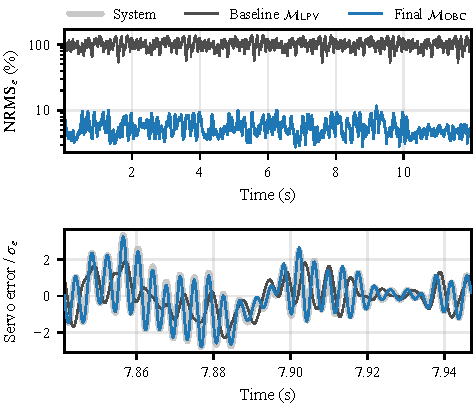
\includegraphics[width=\columnwidth]{res_time_trace.pdf}
  % FEEDBACK (own, 2026-10-24): top is a local NRMS_e; bottom curves are servo errors of system and models (Dirk 2026-10-24).
  \caption{Test record I1, $Y$ axis. Top: $\mathrm{NRMS}_e$ of \eqref{eq:setup_rms} over 50~ms. Bottom: servo error $y-r$ of the system and $\hat y-r$ of the models, divided by $\sigma_{e,Y}$.}
  \label{fig:res_time_trace}
\end{figure}

% FEEDBACK (own, 2026-10-24): float regenerated from Results/24-10-2026/CSV in the agreed design (results preview, Dirk 2026-10-24); running text not yet updated.
\begin{figure}[t]
  \centering
  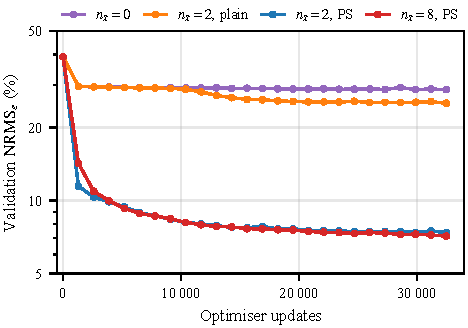
\includegraphics[width=\columnwidth]{res_val_curves.pdf}
  % FEEDBACK (own, 2026-10-24): semicolon replaced (no semicolons, Dirk).
  \caption{Validation $\mathrm{NRMS}_e$ during training, mean over the validation records and axes. Update 0 equals the baseline.}
  \label{fig:res_val_curves}
\end{figure}

\begin{figure}[t]
  \centering
  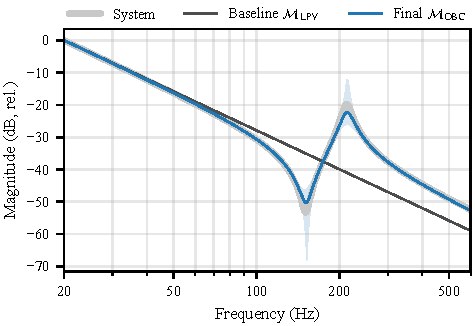
\includegraphics[width=\columnwidth]{res_frf.pdf}
  % FEEDBACK (own, 2026-10-24): open loop, from the linearised models, no normalisation, band range in Y_tr (Dirk 2026-10-24).
  \caption{Open-loop Bode magnitude from $F_Y$ to $Y$ at $Y=0$, from the models linearised at standstill. Shaded: final model over $\lvert Y\rvert\le1.3\,Y_{\mathrm{tr}}$.}
  \label{fig:res_frf}
\end{figure}
% REMOVED (own, 2026-10-24): revnote proposing a figure of the resonance against Y; the text states
%   the frequency and damping range instead.

% Floats stay in their own subsection (Dirk 2026-10-24).
\FloatBarrier
\subsection{Interpretability}\label{sec:res_obc}
\ifdraft
\begin{itemize}
\item Combination errors, full model, physical part and overlaps, $\mathcal M_{\mathrm U}$ against $\mathcal M_{\mathrm{OBC}}$ from the detuned start (Table~\ref{tab:res_obc})
\item Correct start and the models without added states in the appendix
\item Uniqueness from the two starts (?: row requested, revnote at the end)
\end{itemize}
\fi
% FEEDBACK (own, 2026-10-24): subsection opens with what it tests (Hoekstra 2026 Sec. 6.3), wording of Section VI-D.
\add[own]{\kwtwo{For Aspect~2, we compare the estimates of $\mathcal M_{\mathrm{OBC}}$ and $\mathcal M_{\mathrm U}$.}}
% FEEDBACK (own, 2026-10-24): sentences in the order of the criteria (uniqueness, accuracy, constraint), then
%   the truth after the overlap that explains it; "compares ... with ..." repeated the opening (Dirk 2026-10-24).
Table~\ref{tab:res_obc} \chg[own]{compares $\mathcal M_{\mathrm{OBC}}$ with
$\mathcal M_{\mathrm U}$, both from the detuned start (Aspect~2)}{\kwtwo{gives the estimates from the detuned and the true start}}.
\delmv[own]{below}{Both models have deviated further from the true combinations, than their initial values.}
\del[own]{$\mathcal M_{\mathrm U}$ deviates close to double that of $\mathcal M_{\mathrm{OBC}}$.}
\delmv[own]{below}{The combinations describing the damping deviate the most,
while the mass combinations stay close to their true values.}
% FEEDBACK (own, 2026-10-24): uniqueness from the two starts, the criterion of Section I.
\add[own]{\kwtwo{The estimates of $\mathcal M_{\mathrm{OBC}}$ from the two starts differ by 31.3\,\%, while those of $\mathcal M_{\mathrm U}$ differ by 36.4\,\%.}}
% FEEDBACK (own, 2026-10-24): OBC is 0.6 points worse on X (Table res_obc_constraint).
The final model with the orthogonality constraint and the unconstrained model
\chg[Dirk]{perform equally well}{\kwtwo{have similar performance}}.
% FEEDBACK (own, 2026-10-24): Table res_obc_constraint referenced; "From the correct start" struck,
%   no longer true in the final CSVs (59.5 against 58.3).
% FEEDBACK (own, 2026-10-24): overlap 0.00 on training, 0.24 on test; "However" links the limitation (Dirk 2026-10-24).
\kw{OBC keeps the network out of the parameter directions\add[own]{\kwtwo{ on the training records}}: its network overlap is
much lower than that of $\mathcal M_{\mathrm U}$\add[own]{\kwtwo{ (Table~\ref{tab:res_obc_constraint})}}.
% FEEDBACK (Dirk, 2026-10-25): validation row added to Table res_obc_constraint; overlap on all splits.
\add[Dirk]{\kwtwo{The network overlap of $\mathcal M_{\mathrm{OBC}}$ is also much lower than that of $\mathcal M_{\mathrm U}$ on the validation and test records.
It increases from 0.00 on the training records to 0.24 on the test records.}}
\chg[own]{The}{\kwtwo{However, the}} missing dynamics are not orthogonal to these directions, their overlap is 0.59.
\del[own]{From the correct start, OBC also ends closer to the true values (Appendix~\mbox{\ref{app:choices}}).}
\delmv[own]{below}{Without added states, $\mathcal M_{\mathrm U}$ ends closer instead.}}
\mv[own]{above}{Both models have deviated further from the true combinations\del[own]{,} than their initial values.}
% FEEDBACK (own, 2026-10-24): final numbers (Results/24-10-2026/CSV): 83.1 against 69.1 is not double.
\add[own]{\kwtwo{With the detuned start, $\mathcal M_{\mathrm U}$ deviates 83.1\,\% from the true values and $\mathcal M_{\mathrm{OBC}}$ 69.1\,\%.}}
% FEEDBACK (own, 2026-10-24): the only reference to Table app_obc_na0; after the detuned numbers it contrasts with.
\mv[own]{above}{Without added states, $\mathcal M_{\mathrm U}$ ends closer instead\add[own]{\kwtwo{ (Table~\ref{tab:app_obc_na0})}}.}
\mv[own]{above}{The \add[Dirk]{\kwtwo{parameter }}combinations describing the damping deviate the most,
while the mass combinations stay close to their true values.}
% FEEDBACK (own, 2026-10-24): verdict for Aspect 2 with its reason (Maarten: argue every result).
% FEEDBACK (own, 2026-10-25): "OBC does not make the estimates unique" contradicted Section IV (unique
%   for the one-step error) and Maarten p15; observation only (Dirk 2026-10-25).
\add[own]{\kwtwo{\chg[own]{OBC does not make the estimates unique, because they still depend on where training starts.}{The estimates of both models still depend on where training starts.}}}

% FEEDBACK (own, 2026-10-24): float regenerated from Results/24-10-2026/CSV in the agreed design (results preview, Dirk 2026-10-24); running text not yet updated.
%   tab:app_obc_full (cut from the appendix) is kept as a second label: this table now holds both starts.
\begin{table}[t]
  \centering
  % FEEDBACK (own, 2026-10-24): "after training" and the comma chain replaced (Dirk 2026-10-24).
  \caption{Relative error of the ten estimated combinations of $\mathcal M_{\mathrm U}$ and $\mathcal M_{\mathrm{OBC}}$, trained from the detuned and from the true start. Distances: Euclidean norm over the ten combinations.}
  \label{tab:res_obc}\label{tab:app_obc_full}
  \setlength{\tabcolsep}{3pt}
\begin{tabular}{l r r r r r}
\toprule
 & & \multicolumn{2}{c}{$\mathcal{M}_{\mathrm{U}}$} & \multicolumn{2}{c}{$\mathcal{M}_{\mathrm{OBC}}$}\\
\cmidrule(lr){3-4}\cmidrule(lr){5-6}
Rel.\ error (\%) & Initial & Detuned & True & Detuned & True\\
\midrule
$k_{b,\Sigma}$ & $-10.0$ & $-21.8$ & $-7.6$ & $-7.1$ & $-9.7$\\
\midrule
$c_{g1}$ & $+10.0$ & $+45.6$ & $+27.7$ & $+34.0$ & $+23.6$\\
$c_{g2}$ & $+10.0$ & $+45.9$ & $+27.2$ & $+28.4$ & $+16.2$\\
$c_y$ & $+10.0$ & $+43.3$ & $+29.5$ & $+47.4$ & $+34.1$\\
$c_{b,\Sigma}$ & $-10.0$ & $+14.7$ & $+29.2$ & $+21.8$ & $+35.7$\\
\midrule
$m_h$ & $-10.0$ & $-1.3$ & $+1.4$ & $-2.0$ & $+1.8$\\
$m_\Sigma$ & $+10.0$ & $+2.6$ & $+1.3$ & $+0.5$ & $-0.6$\\
$m_\Delta$$^*$ & $-0.5$ & $-0.5$ & $-0.1$ & $-2.1$ & $-1.6$\\
$J_{\mathrm{eff}}$ & $-10.0$ & $-2.2$ & $+4.1$ & $-2.7$ & $+4.7$\\
\midrule
$d$ & $-10.0$ & $-11.7$ & $-9.1$ & $+3.7$ & $-12.7$\\
\midrule
Norm to truth & $30.0$ & $83.1$ & $58.3$ & $69.1$ & $59.5$\\
Start difference &  & \multicolumn{2}{c}{$36.4$} & \multicolumn{2}{c}{$31.3$}\\
\bottomrule
\multicolumn{6}{l}{\footnotesize $^*$ relative to the mean actuator mass, because its true value is close to zero.}\\
\end{tabular}

\end{table}

% FEEDBACK (own, 2026-10-24): float regenerated from Results/24-10-2026/CSV in the agreed design (results preview, Dirk 2026-10-24); running text not yet updated.
\begin{table}[t]
  \centering
  % FEEDBACK (own, 2026-10-24): physical-part rows removed from the table and caption (Dirk 2026-10-24).
  % FEEDBACK (own, 2026-10-24): accuracy rows average all test records, unlike Table tab:res_structure; caption says so (float critique, Dirk yes).
  % FEEDBACK (own, 2026-10-24): comma chain replaced; NRMS_e over the records of Table res_structure (Dirk 2026-10-24).
  \caption{Overlaps of \eqref{eq:obc_overlap} and $\mathrm{NRMS}_e$ of $\mathcal M_{\mathrm U}$ and $\mathcal M_{\mathrm{OBC}}$, trained from the detuned start. The $\mathrm{NRMS}_e$ is the mean over the records with and without multisine.}
  \label{tab:res_obc_constraint}
  \setlength{\tabcolsep}{4pt}
\begin{tabular}{l r r}
\toprule
 & $\mathcal{M}_{\mathrm{U}}$ & $\mathcal{M}_{\mathrm{OBC}}$\\
\midrule
$\rho(F_{\mathrm{aug}})$, training records & $0.85$ & $0.00$\\
$\rho(F_{\mathrm{aug}})$, interpolation test records & $0.84$ & $0.24$\\
$\rho(\Xi)$, interpolation test records & \multicolumn{2}{c}{$0.59$}\\
\midrule
\multicolumn{3}{l}{$\mathrm{NRMS}_e$ (\%), test records}\\
$X_1$ & $5.7$ & $6.3$\\
$X_2$ & $5.6$ & $6.2$\\
$Y$ & $4.8$ & $4.6$\\
\bottomrule
\end{tabular}

\end{table}
% REMOVED (own, 2026-10-24): revnote asking for a figure of the combinations from both starts; Dirk
%   prefers the table, which now holds both starts and the start difference.

% Floats stay in their own subsection (Dirk 2026-10-24).
\FloatBarrier
\subsection{Generalisation}\label{sec:res_generalisation}
\ifdraft
\begin{itemize}
\item Final model, baseline and black box per test record, each E record beside its I record (Fig.~\ref{fig:res_generalisation})
\item Multisine twins of the records without multisine
\end{itemize}
\fi
% FEEDBACK (own, 2026-10-24): subsection opens with what it tests (Hoekstra 2026 Sec. 6.3), wording of Section VI-D.
\add[own]{\kwtwo{For Aspect~3, we compare the final model with the baseline and the black box on the interpolation (I) and extrapolation (E) records (Table~\ref{tab:res_generalisation}).}}
% FEEDBACK (own, 2026-10-24): one sentence per finding, not per table cell; the table pointer is in the
%   opening; Dirk's two sentences with two corrections (E is up to 0.5 points lower on X; the black box
%   is better than the baseline on Y with multisine) (Dirk 2026-10-24).
\del[own]{The error per test record are shown in Fig.~\mbox{\ref{fig:res_generalisation}},
for extrapolation (E) and interpolation (I) (Aspect~3).}
\add[Dirk]{\kwtwo{The errors between E and I differ only by at most 0.5 points.}}
Without multisine the model performs \chg[own]{as well or slightly above}{\kwtwo{as well as or slightly worse than}} the baseline.
\chg[own]{The black box has 74 to 193\,\% on the records without multisine, and it is
below the final model only on I2 $X_2$.}{\kwtwo{The black box is worse than the final model with and without multisine, and reaches 97 to 128\,\% without it.}}
\add[Dirk]{\kwtwo{It even performs worse than the baseline model, except on $Y$ with multisine.}}
\chg[own]{On the \kw{multisine twins}, the final model stays below 10\,\% on $Y$, while the
baseline and the black box are above 47\,\%.}{\kwtwo{With multisine, the final model stays below 8\,\% on all axes, while the errors of the baseline and the black box exceed 65\,\% on $Y$.}}
% FEEDBACK (own, 2026-10-24): verdict for Aspect 3 with its condition (Maarten: argue every result).
\add[own]{\kwtwo{The final model generalises to the held-out positions and unseen motion profiles, but only improves on the baseline when the multisine excites the missing dynamics.}}
% REMOVED (own, 2026-10-24): revnote on the generalisation figure; the figure is now Table
%   res_generalisation.

% FEEDBACK (own, 2026-10-24): float regenerated from Results/24-10-2026/CSV in the agreed design (results preview, Dirk 2026-10-24); running text not yet updated.
%   The per-record figure is replaced by this table (Dirk 2026-10-24); fig:res_generalisation is kept as a
%   second label so the notes that still name it resolve.
\begin{table}[t]
  \centering
  % FEEDBACK (own, 2026-10-24): the number of records differs per column; caption gives it (float critique, Dirk yes).
  % FEEDBACK (own, 2026-10-24): every record with a multisine in one group (Dirk 2026-10-24).
  % FEEDBACK (own, 2026-10-24): record counts dropped, Table res_structure gives them (Dirk 2026-10-24).
  \caption{$\mathrm{NRMS}_e$ per axis on the test records, mean over the interpolation (I) and extrapolation (E) records with and without a multisine.}
  \label{tab:res_generalisation}\label{fig:res_generalisation}
  \setlength{\tabcolsep}{3pt}
\begin{tabular}{l l r r r r}
\toprule
 & & \multicolumn{2}{c}{Multisine} & \multicolumn{2}{c}{No multisine}\\
\cmidrule(lr){3-4}\cmidrule(lr){5-6}
$\mathrm{NRMS}_e$ (\%) & & I & E & I & E\\
\midrule
$\mathcal{M}_{\mathrm{LPV}}$ & $X_1$ & $14.3$ & $12.3$ & $4.5$ & $4.1$\\
 & $X_2$ & $14.6$ & $12.0$ & $4.6$ & $4.1$\\
 & $Y$ & $89.5$ & $78.0$ & $3.4$ & $3.1$\\
\midrule
$\mathcal{M}_{\mathrm{OBC}}$ & $X_1$ & $7.9$ & $7.5$ & $4.7$ & $4.3$\\
 & $X_2$ & $7.3$ & $6.8$ & $4.7$ & $4.3$\\
 & $Y$ & $6.1$ & $6.3$ & $3.8$ & $3.5$\\
\midrule
$\mathcal{M}_{\mathrm{BB}}$ & $X_1$ & $78.5$ & $82.4$ & $104.8$ & $108.5$\\
 & $X_2$ & $79.2$ & $81.1$ & $97.0$ & $99.8$\\
 & $Y$ & $65.9$ & $74.7$ & $127.7$ & $127.0$\\
\bottomrule
\end{tabular}

\end{table}


% Floats stay in their own subsection (Dirk 2026-10-24).
\FloatBarrier
\subsection{Discussion}\label{sec:discussion}
% FEEDBACK (Dirk, 2026-10-24): Discussion rewritten with Dirk in the chat, one paragraph per aspect
%   plus limits, from his own sentences (Hoekstra 2026 Sec. 6.3 and 7.4 as model); new: integrators,
%   controller rate (D-265), controller hides overlap, black box against grey box. Numbers from
%   Results/24-10-2026/CSV. Answers M-p15b (separate subsection), M-p15c, M-p15e, M-p15f, Q-p9.
%   The old text is kept below as commented-out source.
%   Marks (2026-10-24, Dirk): black = Dirk's own sentences, red = new or changed words only.
% FEEDBACK (own, 2026-10-25): Discussion rewritten below one column (Dirk 2026-10-25: two columns
%   way too much), with a test for each point, the future work and the root cause link. Second pass
%   in Dirk's wording (Dirk 2026-10-25: "I want it in my words"): black = Dirk's own sentences from
%   the earlier Discussion and Sections V to VII, red = new, written in his patterns (subject first,
%   "We" + plain verb, purpose with "to", reason after "since" or "because", "is able to",
%   "A possible cause is", contrast with ", but", "instead of", tables in brackets at the end).
%   Third pass (Dirk 2026-10-25: Sections I and II were not used): red sentences redone with the
%   patterns of Sections I and II as well ("However," and "Therefore" at the start, "meaning that",
%   "This does not ..., but", "We have chosen ..., so that", "a deviation can indicate which
%   physical parameter has changed" from Section I).
%   Merged discussion list A1 to A5, A8 to A10, A12, A14. The paragraph-by-paragraph rebuild of
%   2026-10-25 is kept below as commented-out source, above the 2026-10-24 version.
% FEEDBACK (own, 2026-10-25): limited to Y (on X the static correction already gives most of the
%   gain, 13.3 to 9.5 against 7.7 %); evidence is the static correction, which cannot represent a
%   mode (Dirk 2026-10-25).
The improvement on \chg[own]{the multisine records}{\kwtwo{$Y$ with multisine}} is mainly caused
by the learned absorber mode\add[own]{\kwtwo{ (Fig.~\ref{fig:res_frf})}}.
\add[own]{\kwtwo{The static correction without added states, 
is only able to lower the error on $Y$ from 83.7\,\% for the baseline to 60.4\,\%,
while two added states with PS reach 6.1\,\% (Table~\ref{tab:res_structure}).
Training without PS does not seem to find this mode in the current setting, it stays above 50\,\%.}}
Without multisine, the final model performs slightly worse than the baseline.
For these records the baseline error is only a few percent of the serve error, 
and only four of the eighteen training records are 
without multisine. Resulting in the records without multisine contributing relatively little 
to the loss.
The final model remains far above the noise floor on every record.
A possible reason is that the relative error is already small, 
so reducing it further requires a better tuned optimisation.
The augmentation might not be able to capture the unmodelled friction, or the 
difference in controller rates contributes to this.
From these results, we cannot conclude what the reason is.
\\
OBC is able to keep the neural network out of the parameter
directions on the training tuples, and for the most part on the validation and test records
compared to $\mathcal M_{\mathrm U}$ (Table~\ref{tab:res_obc_constraint}).
However, the missing dynamics are not orthogonal to these directions, 
their overlap is 0.59 (Table~\ref{tab:res_obc_constraint}).
Orthogonality is defined to hold only to first order and at $\bar x=0$, 
and the added states enter through $f_{\mathrm{aug}}$ without projection.
This holds for a single step, not for the simulated output, 
where the model is simulated over multiple steps with nonzero added states.
Even when training starts from the true parameters, the
damper combinations deviate the most, while the mass combinations stay close
to their true values (Table~\ref{tab:res_obc}).
A possible explanation is that the dampers absorb part of the friction, 
since both produce a force in the opposite direction of the velocity.
For both models, the estimates from the two starts differ by a similar amount (Table~\ref{tab:res_obc}),
so the trained estimate still depends on the start.
Given the current results, 
the estimates cannot be used to trace a change in the machine back to a physical parameter.
\\
For the interpolation and extrapolation records both the baseline and the final model 
have a similar error (Table~\ref{tab:res_generalisation}), 
However, most extrapolation records extend beyond the training range in only one direction.
The black box model underperforms, while we would expect it to have similar results to the grey box model, 
as in~\cite{hoekstra2026lfr}.
Possible reasons for the underperformance are that it starts from a random initialisation, 
instead of for example a best linear approximation.
The black box model also has to learn the controller dynamics, because
the controller is not included in the training loop.
What we do see is that the black box model performs much better on the records with multisine than on the records without (Table~\ref{tab:app_splits}).
For the records without multisine, the reference is the only input.
The black box model therefore has to learn the complete closed-loop response, while the grey box model uses the known controller and starts from the baseline.
\\
The results are limited to simulation with one seed and the
same controller used to generate the data.
Training and evaluation are both performed in closed loop, 
where the controller can suppress errors in the plant model.
A different controller might be able to reveal these errors. 
The recorded input is correlated with the measurement noise through the feedback, 
while SUBNET assumes they are independent~\cite{beintema2023subnet}.
Therefore, we have not shown the consistency of the estimate.
\\
For future work, the model should be evaluated on measured data, and evaluated with a different controller.
OBC could also be extended to the simulated output, using its Jacobian over a training window instead of the Jacobian of a single state update.
% PREVIOUS Discussion (paragraph-by-paragraph rebuild, 2026-10-25), replaced by the text above:
% The improvement on the multisine records comes mainly from the
% learned absorber mode\add[Dirk]{\kwtwo{, which needs both the added states and their PS
% initialisation}} (Fig.~\ref{fig:res_frf}\add[Dirk]{\kwtwo{, Table~\ref{tab:res_structure}}}).
% % FEEDBACK (own, 2026-10-25): paragraph 1 rebuilt in the pattern of Hoekstra 2026 Secs. 6.3 and 7.4
% %   (claim, why, limit, test), merged discussion list A1, A2; damping-over-Y sentence cut, no float
% %   shows it (Dirk 2026-10-25).
% \add[own]{\kwtwo{With the same two added states, plain training keeps the
% error on $Y$ above 50\,\%, so the added states can represent the mode,
% but training only finds it from the PS start.}}
% Without multisine, the final model performs slightly worse than the baseline.
% \add[own]{\kwtwo{These records contribute little to the loss, because the
% loss weights each record by its own servo error, on which the baseline
% already reaches a few percent, against up to 120\,\% on the records with
% multisine.}}
% \add[own]{\kwtwo{The final model is also slightly worse on the training
% records without multisine (Table~\ref{tab:app_splits}), so this is not
% overfitting.}}
% % FEEDBACK (Dirk, 2026-10-24): review: observation first, the integrators as a possible cause only.
% % FEEDBACK (own, 2026-10-25): free integrators struck (closed loop is stable); controller rate kept as
% %   a candidate beside friction, with the test that separates them (Dirk 2026-10-25).
% \add[Dirk]{\kwtwo{Both models stay far above the noise floor on these records.
% \del[own]{A possible cause is the free integrators on $X$ and $Y$, which accumulate
% small errors.}
% \chg[own]{The training simulates the controller at 4~kHz, while the data are generated
% with the controller at 20~kHz.
% The augmentation can therefore learn part of this difference as plant
% dynamics.}{Possible causes are the unmodelled friction and the controller,
% which runs at 4~kHz in training and at 20~kHz in the data.
% The results do not separate these causes, but retraining with more weight
% on these records, or on data without friction, would.}}}
% \\
% OBC reduces the \del[Dirk]{final }combination error compared with the
% unconstrained model (69.1 against 83.1\,\%), but the parameters still end up
% further from the truth than at their initial values (Table~\ref{tab:res_obc}).
% % FEEDBACK (own, 2026-10-24): approved wording changes: separate the recovery explanation and name the comparison.
% % FEEDBACK (own, 2026-10-25): paragraph 2 rebuilt (claim, why, limit, test), merged discussion list
% %   A3 to A6: "holds" restricted to the training tuples (test overlap 0.24); why the parameters move
% %   from the true start, with friction and added mass as candidates; controller sentence moved to the
% %   limits paragraph (untested); start corrected (Table app_obc_na0 uses the detuned start); two-start
% %   limit (Maarten p14); projection sentence made precise; root-cause consequence (Dirk 2026-10-25).
% \add[Dirk]{\kwtwo{The constraint holds\add[own]{ on the training tuples}, but the missing dynamics are not orthogonal to the
% parameter directions\chg[own]{ (truth overlap 0.59)}{. Their overlap is 0.59}, so the recovery condition of
% Section~\ref{sec:obc_ident} is not met\del[own]{ and the parameters are biased}.
% \add[own]{This explains why the true values are not recovered, but not where
% the parameters end: even from the true start both models move far from the
% true values, mostly in the damper combinations, while the mass combinations
% stay close.
% Both the friction, which dissipates energy as the dampers do, and the added
% mass are candidates for what the dampers absorb.
% Training on data with only one of them would separate the two.}
% \delmv[own]{limits paragraph}{In closed loop, the controller can also hide the effect of this bias on the
% output.}
% \chg[own]{From the correct start and without added states}{Without added states}, OBC does not end closer to
% the true values\add[own]{ than the unconstrained model}\add[own]{ (Table~\ref{tab:app_obc_na0})}.}}
% With OBC the estimates from the \chg[Dirk]{true and detuned}{\kwtwo{two}} starts are closer together, but still
% differ\add[Dirk]{\kwtwo{ (31.3 against 36.4\,\%)}}.
% \add[own]{\kwtwo{With two starts and one training run each, this cannot separate
% a remaining dependence on the start from incomplete convergence.
% Training from several starts and seeds would.}}
% % FEEDBACK (Dirk, 2026-10-24): review: observation and possible reason separated (Dirk's two
% %   sentences); no uniqueness claim either way (Section IV, M-p15e).
% \chg[own]{The orthogonality holds only to first order and at $\bar x=0$, and the added
% states enter through $f_{\mathrm{aug}}$ without projection.}{\kwtwo{The projection
% is fitted to first order and at $\bar x=0$ on the training tuples, so the
% effect of the added states on $f_{\mathrm{aug}}$ is not removed.
% On the test records the network overlap rises to 0.24
% (Table~\ref{tab:res_obc_constraint}).}}
% \add[Dirk]{\kwtwo{OBC therefore reduces the dependence on the start, but does not recover
% the true values.}}
% \add[own]{\kwtwo{Only the mass combinations can therefore be read physically.
% A change in the damper estimates cannot indicate a change in the machine,
% which limits the root cause analysis of Section~\ref{sec:intro}.}}
% \\
% % FEEDBACK (own, 2026-10-25): paragraph 3 rebuilt (claim, why, limit, test), merged discussion list
% %   A8, A9: "all" -> on average (E1 is worse than I2 per record, CSV only); baseline equally good on
% %   E, so a weak test; E5 exceeds several limits; black box poor without multisine only, best update
% %   78000 of the 80000 budget; it fails on the reference motion; comparison shows prior knowledge,
% %   with the test that separates the causes (Dirk 2026-10-25).
% \chg[own]{The final model maintains its accuracy on all extrapolation
% records\add[Dirk]{\kwtwo{, but}} each record extends beyond the training range in only one
% direction}{\kwtwo{On average, the final model maintains its accuracy on the
% extrapolation records}} (Table~\ref{tab:res_generalisation}).
% \add[own]{\kwtwo{The baseline is not worse on these records either, so they
% test the extrapolation of the learned part only weakly.
% Most extrapolation records exceed one limit in one direction, and only E5
% exceeds several.
% Records further outside the training range, and on both sides of it, would
% test it more strongly.}}
% The black box model performs poorly on its training records \chg[own]{and \chg[Dirk]{had not converged}{\kwtwo{did not converge}} within the available budget}{\kwtwo{without multisine,
% and its best checkpoint lies at the end of the training budget, so it was
% still improving}} (Table~\ref{tab:app_bb_search}).
% \add[own]{\kwtwo{With multisine it performs much better
% (Table~\ref{tab:app_splits}).
% It therefore fails on the reference motion: it must learn how the closed
% loop turns the large reference into the small servo error, which the grey
% box obtains from the known controller and the baseline.}}
% % FEEDBACK (own, 2026-10-24): approved wording change: separate parameter initialisation from controller use.
% \chg[own]{It is also randomly initialised and
% trained without the controller, while the grey box
% starts from the baseline with the controller in the loop}{\kwtwo{The black box model starts from randomly initialised parameters, while the
% grey box starts from the physics baseline.
% The black box is also trained without the controller}}.
% \add[own]{\kwtwo{The comparison therefore shows the value of this prior
% knowledge, not a limit of black-box models.
% A black box of the plant inside the known loop, with a linear
% initialisation and a longer budget, would separate these causes.}}
% \\
% % FEEDBACK (own, 2026-10-25): paragraph 4 rebuilt, merged discussion list A10, A12 to A14: which
% %   claim the seed limits; feedback below the crossover, added mass above it by design (Section V);
% %   controller-hides-bias sentence from the interpretability paragraph returns as a possibility;
% %   changed-controller use untested (Section I); favourable simulated setting and the research-plan
% %   departure (validation on the machine); future work (Dirk 2026-10-25).
% The results are limited to simulation with one seed and the
% same controller used to generate the data.
% \add[own]{\kwtwo{With one training run per model, differences of about one
% point, such as between $\mathcal M_{\mathrm{OBC}}$ and $\mathcal M_{\mathrm U}$,
% are not resolved.
% The feedback suppresses plant errors below the crossover, while the added
% mass lies above it by design (Section~\ref{sec:setup_loop}), so the results
% show the accuracy above the crossover.
% Below it the controller can hide plant errors, possibly including the
% parameter bias discussed above.
% The use that motivates this thesis, evaluating a changed controller
% (Section~\ref{sec:intro}), is therefore not tested.
% Simulating the trained model with a second controller would test it.}}
% Through the feedback, the recorded input is correlated with the measurement
% noise, so the consistency of the \add[Dirk]{\kwtwo{SUBNET }}estimate\add[Dirk]{\kwtwo{~\cite{beintema2023subnet}}} is
% not shown.
% \add[own]{\kwtwo{The simulated system adds a chosen added mass and friction to
% the baseline, with an excitation designed from its known response, which is
% a favourable setting, while the research plan foresaw validation on the
% machine.}}
% It remains unclear whether the improvements would hold with a different
% controller or on measured data.
% \add[own]{\kwtwo{Future work is to include the friction in the baseline, to
% extend the projection to the added states, and to evaluate the model on
% measured data.}}
% OLD Discussion (until 2026-10-24), replaced by the four paragraphs above:
% \todo{Should this be a separate subsection? Didnt Maarten state to include it in the text itself...?}
% % RESTRUCTURE (2026-10-19, Maarten p15): moved here from Section VIII (sec:conclusion), word for word.
% \mv[M-p15]{VIII}{The improvement on the multisine records comes mainly from the
% learned absorber mode (Fig.~\ref{fig:res_frf}).
% The results in Table~\ref{tab:app_structure} (Appendix~\ref{app:choices})
% show that both the added states and their PS initialisation are needed
% to obtain this improvement.
% Without multisine, the final model performs slightly worse than
% the baseline.
% The baseline is already accurate on these records, so the learned
% correction might overfit on the multisine records
% and introduce small errors on the records without multisine.
% \revnote{Issue: without multisine the final model stays at the level of
% the baseline (3.8 against 3.4\,\% on $Y$), far above the noise floor.
% The data give no sign that the friction is learned, but they also do not
% show that the remaining error is caused by friction.
% Question: is ``consistent with the unmodelled friction'' the right
% wording for this remaining error?}
% \\
% % FEEDBACK (own, 2026-10-24): final R1 norm (Results/24-10-2026/CSV/res_obc_combinations.csv,
% %   D-259 scaling); final R2 59.5 % against R5 58.3 % from the correct start.
% % FEEDBACK (Dirk, 2026-10-24): the constraint holds, but the missing dynamics are not
% %   orthogonal to the baseline; selection uses the validation error only, because the
% %   truth is unknown. The todo "Use this?" is answered: the sentence is kept.
% OBC reduces the final combination error compared with the
% unconstrained model (\chg[own]{47.7}{\kwtwo{69.1}} against 83.1\,\%), but the parameters
% still end up further from the truth than at their initial values
% (Table~\ref{tab:res_obc}).
% \chg[own]{The missing dynamics have a truth overlap of 0.59 with the
% parameter directions.
% The truth overlap of 0.59 means}{\kwtwo{The network overlap of OBC is much lower than that of
% the unconstrained model, which shows that the constraint holds.
% The missing dynamics themselves are not orthogonal to the parameter directions.
% Their truth overlap is 0.59.
% This means}} $\Phi^\top\Xi\neq0$, \chg[own]{so the recovery
% condition of Section~\mbox{\ref{sec:obc_ident}} is not met and OBC is not
% expected to recover the true values.}{\kwtwo{and the recovery condition of
% Section~\ref{sec:obc_ident} is not met.
% OBC keeps this part of the missing dynamics out of the network, and the
% physical parameters absorb it instead.
% From the correct start, OBC therefore also moves away from the true values
% (Table~\ref{tab:app_obc_full}).}}
% The orthogonality holds only to first order and at $\bar x=0$.
% During training, the added states enter the physical states through
% $f_{\mathrm{aug}}$ without projection.
% This is a limitation of imposing the constraint at $\bar x=0$.
% \add[own]{\kwtwo{The model is selected on the validation error only
% (Section~\ref{sec:aug_closed_loop}), because the true parameters are unknown
% outside simulation.
% A small decrease in the validation error can therefore come with a large
% drift of the damper combinations.}}
% With OBC the estimates from the true and detuned starts are closer together, 
% but still differ (Table~\ref{tab:app_obc_full}).
% The results therefore show less dependence on initialisation,
% but does not establish uniqueness.
% \\
% The black box model performs poorly on its training records and
% had not converged within the available budget
% (Table~\ref{tab:app_bb_search}).
% % The final model maintains its accuracy on all extrapolation
% % records (Fig.~\ref{fig:res_generalisation}).
% % However, each record extends beyond the training range in only
% % one direction, so the results do not establish how the model
% % behaves further outside this range.
% The black box model is also randomly initialised and not trained 
% with the known controller.
% Having a disadvantages starting position. t
% \\
% % NEW (2026-10-20, Dirk; LFR audit): role of the LPV-LFR, in the text so it
% %   survives submission (the revnote does not).
% % RESTRUCTURE (2026-10-22, Dirk): the LFR derivation is now in Appendix A.2;
% %   III-B gives the baseline transition eq:base_ss.
% \kwtwo{The baseline is represented as an LPV-LFR \chg[Dirk]{(Section~\mbox{\ref{sec:lfr}})}{(Appendix~\ref{app:lfr-details})},
% which is well posed for admissible physical parameters.
% The implementation resolves its loop analytically, and the learned correction
% is added to the resulting discrete-time state update.
% The augmentation therefore uses the baseline transition, but does not connect
% to the latent signals of the LFR.
% The augmented model is evaluated in closed-loop simulation; LPV controller
% synthesis with this model is outside the scope of this work.}
% \\
% The results are limited to simulation with one seed and the
% same controller used to generate the data.
% Training and evaluation are both performed in closed loop,
% where the controller can suppress errors in the plant model.
% \kwtwo{Through the feedback, the recorded input is correlated with the
% measurement noise\add[own]{, while SUBNET assumes an input that is
% independent of the noise~\cite{beintema2023subnet}}, so the consistency
% of the estimate is not shown.}
% % FEEDBACK (own, 2026-10-21): SUBNET's independence assumption is stated in
% %   IV-C (Beintema 2023 Sec. 2.1); the correlation is stated in Section II
% %   (Dirk 2026-10-21).
% It remains unclear whether the improvements would hold with
% a different controller or on measured data.}
% REVNOTE (2026-10-20, Dirk): role of the LFR; checked against
%   blocks.py Gantry_State_Block (closed-form loop, then G and Delta) and
%   Drenth 2025 (paper Sec. 1, thesis Ch. 1: LPV-LFR for controller synthesis).
% The explanation is now in the paragraph above (2026-10-20); the revnote
%   keeps only the question.
% REVNOTE closed (2026-10-22, Dirk): "Should the LPV-LFR derivation stay as
%   a compact subsection in the main text?" No: it moved to Appendix A.2;
%   III-B states the baseline transition and points to the LFR.

% Open points of this section (kept together so the text reads without interruption).
\todo{Missing: the numbers of $\mathcal M_{\mathrm{OBC}}$ (R1) in this section
are preliminary (update 19500 of 33400). Candidate: update them after the
final R1/R2 rerun (basis: handoff 2026-10-18, Sec.~3).}
\todo{Missing: the network overlap of $\mathcal M_{\mathrm{OBC}}$ in
Table~\ref{tab:res_obc} comes from update 18200 while labelled 19500, so the
text gives no number for it. Candidate: recheck after the final R1 rerun
(basis: handoff 2026-10-18, Sec.~12).}
\todo{Missing: the caption of Fig.~\ref{fig:res_generalisation} says ``RMS,
mean over $X_1$, $X_2$, $Y$'', while the text reads $\mathrm{NRMS}_e$ per
axis. Candidate: check the figure and update the caption (Jasper p9: say
error of what with respect to what).}
\todo{Are state Gramians useful for explaining each added state's contribution, or would intervention-based ablation be more direct and less linearisation-dependent?}
% \revnote{The ``OBC pred.'' columns are dropped (Dirk 2026-10-18). The
% first-order bias of \eqref{eq:obc_recovery} is 100 to 1300\,\% against
% observed errors of a few to 30\,\%: outside the range of the expansion, and
% it holds for the one-step least-squares fit at $\bar x=0$, not the
% closed-loop training with active added states. The truth overlap row keeps
% the argument why OBC cannot recover the true parameters; the text that
% compares predicted and observed $\delta_j$ (05\_setup, end of the metric
% paragraph) still needs to go.}
% \revnote{Request (2026-10-18): add a row ``difference between starts'' to
% Table~\ref{tab:res_obc}, the norm of $\delta_j$ from the detuned start minus
% $\delta_j$ from the correct start, per arm. Section~\ref{sec:intro} defines
% interpretability as a unique estimate, and this row tests uniqueness; the
% norm to the truth tests recovery. From
% Table~\ref{tab:app_obc_full} by hand (R1, R2 preliminary): 36.4\,\%
% unconstrained, 25.1\,\% OBC. To be computed by
% \texttt{Code/Figures/res\_obc\_combinations.py} after the final R1/R2 rerun.}

% Page budget: 0.90 pages | Owns: answers to the research question, interpretation, limitations, departures, and industrial meaning.
% WRITING GUIDE
% Purpose: Interpret the final evidence, reconcile prediction and interpretability, and state the limits of the conclusions.
% Start here: The frozen Results section and its acceptance criteria.
% Supporting material: Quinten's 18 September outline feedback, the Meeting-audit synthesis, docs/closed-loop-training-findings-2026-08-28.md, supervisor-summary-2026-08-30.md, and newer decisions that confirm or supersede them.
% Research-plan anchor: Answer all four planned aspects and explain why any original expected outcome was not reached or was reformulated.
% Current decisions: Separate local decomposition uniqueness, true-parameter recovery, closed-loop fit, autonomous prediction, interpolation, and extrapolation.
% Choices to justify: Which result is primary, which limitations change the answer, and which unsuccessful choices are scientifically informative rather than implementation history.
% Implementation audit: Recheck every causal explanation against the implemented objective, routing, controller, OBC construction, and diagnostic intervention before stating it as a mechanism.
% Reference check: Cite literature for general interpretation and known limitations; do not use a citation to replace project evidence for what this implementation did.
% Cautions: Do not introduce new results; distinguish limitations demonstrated by evidence from plausible future risks.
% Planned figures: None; interpret figures already introduced.
% Section is finished when: The main research question has a direct answer and each limitation states exactly which claim it restricts.
% Hidden from the review build (2026-10-11): the discussion moved into Section VIII
% (Conclusions and discussion); these bullets stay as source material.
\begin{wip}
\section{Discussion}

\subsection{Answers to the four research aspects}
\begin{itemize}
\item Aspect 1: state whether explicit $Y$ scheduling earns measurable predictive value over frozen LTI baselines
\item Aspect 2: distinguish the expressive value of dynamic augmentation from the observed trainability of its added states
\item Aspect 3: conclude that OBC enforces a unique local split but true parameter recovery is conditional on the real discrepancy's orthogonality and optimiser convergence
\item Aspect 4: compare simulation interpolation, motion-profile transfer, amplitude extrapolation, real-data evidence, and the black-box result without merging them into one score
\item Treat controller transfer as the industrial digital-twin use case and as a closed-loop distribution shift distinct from operating-range extrapolation
\item Interpretability matters when physical parameters support controller redesign or health monitoring, but its practical value must be tied to a named downstream decision
\item Figure plan: introduce no new figure; interpret the architecture, OBC, and result figures already presented instead of adding a summary graphic
\end{itemize}
\todo{Which result is the primary answer if predictive accuracy and parameter recovery favour different arms?}

\subsection{Limitations and lessons}
\begin{itemize}
\item Closed-loop feedback improves numerical trainability but can hide plant mismatch, suppress orthogonality overlap, and reward a model that is poor in open loop
\item Short windows underweight velocity DC bias on free integrators; varying encoder and rollout length is therefore a structural sensitivity test, not routine tuning
\item One strengthened absorber, currently noiseless simulation, a finite neural-seed campaign, and truth-only dry friction bound claims about nonlinear, noisy, and dissipative missing dynamics
\item State the final seed count and corrected-friction evidence here; do not retain development-era caveats after the final campaign changes them
\item Central-difference velocities, force calibration, and the train-validation-test coverage grid bound the credibility of any real-data conclusion
\item The research plan expected validated real-machine generalisation; any missing Telica result is a departure to disclose, not replace with design documentation
\item Augmentation versus residual-FRF fitting remains a trade between trajectory-domain nonlinear prediction and a simpler frequency-domain account of missing dynamics
\item Pointwise orthogonality is impossible for any nonzero missing force on this gantry: the parameter sensitivity of the three velocity rows has rank 3 at every reference sample (worst $\sigma_3/\sigma_1=5.7\cdot10^{-4}$, earlier absorber dataset), so $J^\top\Delta^*=0$ can only arise from cancellation over the record (Section~IV-C)
\item Coulomb friction in the truth violates the recovery condition by construction: the $c_{g1}$ sensitivity is proportional to $\dot X_1$ and the friction is $-c_{c1}\operatorname{sign}(\dot X_1)$, so their inner product is $-c_{c1}\sum|\dot X_1|\neq0$ for any moving record (D-204); on T\_AF, OBC gives a unique split, not unbiased combinations
\item The training loop runs $K_1$ at the model rate instead of the 20~kHz of the data, which changes the feedback force by a median of \SetupKmismatchMed\,\% on the records with multisine and at most \SetupKmismatchMotion\,\% on those without; the model sees a slightly different loop in the band of the added mass (Appendix~\ref{app:setup_checks}) (?: cause, half-sample offset in the reduction or Tustin warping, being checked for the final runs; drop this point if it is fixed)
\end{itemize}
\todo{Should a cubic-spring benchmark, noise study, and Monte Carlo analysis be completed, or should the thesis explicitly narrow its claims to the measured linear absorber case?}
\todo{Missing: the criterion \eqref{eq:aug_loss} weights each axis by $1/\sigma_{y,i}^2$ (normalised outputs, as~\cite[Sec.~5.3]{hoekstra2026lfr}), while checkpoint selection and the reported errors are in metres, so training and evaluation weigh the axes differently. Candidate: one limitation sentence, after checking whether Hoekstra et al.\ (Sec.~6) and Beintema et al.\ report normalised (NRMS) or physical-unit errors (not yet read).}

\subsection{Implications and future work}
\begin{itemize}
\item Design excitation so $J^\top\Delta^*=0$ when true parameter recovery, rather than only a unique decomposition, is required
\item Separate learning rates for physical and neural parameters and compare convergence against the predicted nonzero OBC bias floor
\item Replace the short-horizon objective or couple windows so integrated velocity bias is visible during training
\item Repair and rerun the Coulomb benchmark before claiming that the method learns a legitimate nonzero-mean residual
\item Extend evaluation beyond the multisine range and use machine-relevant trajectories to delimit safe interpolation and extrapolation
\end{itemize}
\todo{Which future-work item is a prerequisite for the thesis claim and which genuinely belongs after graduation?}
\end{wip}

% Page budget: 0.45 pages (conclusion) + 0.90 pages (discussion, from 07) | Owns: interpretation of every result,
%   limits of each claim, departures from the research plan, the answer to the research question.
% WRITING GUIDE
% Purpose: Explain the results that do not speak for themselves, state the limit of each claim, disclose the
%   departures from the research plan, and answer the research question per aspect.
% Start here: the frozen Results section (06) and the method sections it evaluates (03, 04).
% Reference check: introduce no new reference; reuse only verified sources already cited in the method sections.
% Cautions: no new results, runs or figures; every number from a float of 06, the appendix tables or
%   Thesis-writeup/Results/18-10-2026/CSV; untested explanations stated as candidates; no LPV vs LTI as a research
%   result; no predicted-bias comparison; no OBC network-overlap digit (R1 label mismatch).
% Section is finished when: every discussion point is tied to a float and states its limit, and the conclusion
%   answers each aspect and the research question in fewer words than the discussion.
% MUST ESTABLISH (Dirk 2026-10-18; handoff tasks/handoffs/2026-10-18-discussion-conclusion.md)
%   Form: one section "Discussion and Conclusion", discussion first, by aspect as numbered in the Introduction
%   (1 structure and training, 2 OBC interpretability, 3 generalisation), then limits and departures, then a short
%   conclusion in the same order. Results (06) is observational; explanations, limits and departures are here.
%   Interpretability = unique estimate of the identifiable combinations, not true-parameter recovery.
%   Style per paragraph: claim, evidence, limit, what would test it. Conclusion: one or two sentences per aspect,
%   one sentence of the central limit, one recommendation.
%   Checked 2026-10-18: the final runs build the encoder from data (D-271, logs thesis-results-4), so the old
%   "encoder from true parameters" point is no limitation; the K1-rate point of 07 is a diagnostic only (D-265);
%   the axis weighting point of 07 is resolved by W_r and NRMS_e selection (03, eq:aug_loss).
\section{Discussion and Conclusion}\label{sec:conclusion}
\ifdraft
\begin{itemize}
\item Discussion per aspect: explanation, limit and test of each result; then the limits and departures that bound all three (handoff 2026-10-18)
\item Conclusion: the answer per aspect and to the research question, the central limit, one recommendation
\end{itemize}
\fi
This section interprets the results of Section~\ref{sec:results} per aspect,
states the limits of each claim and the departures from the research plan,
and then answers the research question.

\subsection{Augmentation structure}
\ifdraft
\begin{itemize}
\item The gain with multisine is the absorber mode, carried by the network and the added states (Fig.~\ref{fig:res_frf}, Table~\ref{tab:res_obc}, Table~\ref{tab:app_structure})
\item Added states and PS are both needed; shown on validation with one seed (Table~\ref{tab:app_structure})
\item Without multisine the final model is slightly above the baseline; candidates only (Table~\ref{tab:res_structure}) (?)
\end{itemize}
\fi
The gain on the records with multisine comes from the absorber mode.
The final model has a resonance at 2.11 to 2.13\,$f_b$ over $Y$, against
2.12\,$f_b$ of the system (Fig.~\ref{fig:res_frf}).
Its damping ratio is 0.036 to 0.080 over $Y$, against 0.043, so the mode
frequency is learned more accurately than its damping.
With the learned block switched off, the $Y$ error of the trained model
returns to about 42\,\% (Table~\ref{tab:res_obc}), so the network and the
added states carry the mode, not the refitted parameters.
\\
Both the added states and their PS start are needed to learn the mode.
On the validation records with multisine, the $Y$ error is 6.4\,\% with PS,
78.1\,\% with plain training and 86.5\,\% without added states
(Table~\ref{tab:app_structure}).
Eight added states give the same error as two.
This rests on one seed per model, so a seed that lets plain training find
the mode is not excluded.
The missing dynamics hold one mode of known order, so the result shows that
two added states suffice for this mode, not how $n_{\bar x}$ should be
chosen when the order is unknown.
\\
Without multisine, the final model is 0.2 to 0.4 points above the baseline
at the true parameters (Table~\ref{tab:res_structure}).
At this level the baseline misses only the friction and the part of the
absorber that the motion excites.
A candidate explanation is that the learned correction, fitted mainly where
the multisine excites the absorber, adds small errors where the baseline is
already close to its limit.
The detuned start is not the cause: on the validation records, the model
trained from the true parameters is also above the baseline on $Y$
(Table~\ref{tab:app_structure}).
The candidate is not tested.
The error spectrum of both models on these records would show whether the
difference lies in the absorber band or below the crossover.
\todo{Missing: a check of the candidate. Candidate: compare the error spectra of the final model and the baseline on I3 to I6 with the existing evaluation code (no new run; basis: res\_ps\_spectrum uses the same computation on the validation multisine records).}

\subsection{Interpretability}
\ifdraft
\begin{itemize}
\item OBC halves the drift of U but does not recover the truth; expected from the truth overlap and \eqref{eq:obc_recovery} (Table~\ref{tab:res_obc})
\item The dampers move most; the friction projects onto the damping sensitivities by construction (D-204 argument, not measured)
\item OBC holds to first order at $\bar x=0$ for the one-step fit only; added states are not protected
\item Uniqueness only partly shown: the two starts still differ (Table~\ref{tab:app_obc_full}) (?: row requested)
\item Without added states the order reverses; candidate only (Table~\ref{tab:app_obc_na0})
\item Root cause analysis compares unique estimates only while the missing dynamics do not change
\end{itemize}
\fi
OBC reduces the parameter drift, but it does not recover the true
combinations.
From the detuned start, the combination error grows from 30.0\,\% to
47.7\,\% with OBC and to 83.1\,\% without (Table~\ref{tab:res_obc}).
From the correct start, OBC ends at 35.4\,\% and $\mathcal M_{\mathrm U}$ at
58.3\,\% (Table~\ref{tab:app_obc_full}).
This drift is expected from Section~\ref{sec:obc_ident}.
The truth overlap of 0.59 shows that $\Phi^\top\Xi\neq0$ on the tuples, so
the estimate of \eqref{eq:obc_recovery} is biased even with the projection.
OBC costs no accuracy, since the full models and their physical parts differ
by at most 0.9 points between the two arms.
\todo{Missing: the numbers of $\mathcal M_{\mathrm{OBC}}$ (R1, R2) are preliminary (update 19500 of 33400). Candidate: update 47.7, 35.4, 0.9 and the two-start differences after the final rerun (basis: handoff 2026-10-18, Sec.~3).}
\\
The damping combinations $c_{g1}$, $c_{g2}$ and $c_y$ move most, by 23 to
30 points with OBC and 43 to 46 points without, while the mass combinations
stay within 3.4\,\% of their true values.
A candidate cause is the rail friction of \eqref{eq:setup_fric}.
The sensitivity to $c_{g1}$ is proportional to $\dot X_1$, and the friction
force has the sign of $\dot X_1$.
Their inner product over a moving record is therefore nonzero, so the
friction lies partly in the damping directions and biases the dampers
through $\Phi^\top\Xi$.
This argument is ours and is not measured on the final data.
The truth overlap of $\Xi$ split into its friction and absorber parts would
test it.
\\
The guarantee of OBC is also narrower than the training it is applied to.
The projection holds to first order around $\beta_{\mathrm{lin}}$, for the
one-step fit on the reference slice $\bar x=0$
(Section~\ref{sec:obc_ident}).
With PS the added states are active, so the part of $f_{\mathrm{aug}}$ that
depends on $\bar x$ is not orthogonal to the parameter directions, and the
closed-loop criterion \eqref{eq:aug_loss} is not the one-step fit.
The two starts measure how far uniqueness holds in practice.
Their final estimates differ by 25.1\,\% with OBC and 36.4\,\% without, from
Table~\ref{tab:app_obc_full}.
OBC brings the two estimates closer, but they are not equal, so uniqueness is
only partly shown.
\todo{Missing: the two-start difference is computed by hand from Table~\ref{tab:app_obc_full}, not shown in a float. Candidate: the ``difference between starts'' row requested at the end of Section~\ref{sec:results}, computed by \texttt{res\_obc\_combinations.py} after the final rerun.}
\\
Without added states the order reverses: $\mathcal M_{\mathrm U}$ ends at
48.8\,\% and $\mathcal M_{\mathrm{OBC}}$ at 68.4\,\%
(Table~\ref{tab:app_obc_na0}).
A candidate explanation is that the network must then represent the absorber
statically, and a large part of it lies in the parameter directions (truth
overlap 0.59).
The projection removes that part from the network, so the parameters absorb
it.
This is not tested.
The result shows that OBC does not bring the estimate closer to the truth in
general.
Its guarantee is a unique split, and only the pair from two starts tests that.
\todo{Missing: a possible inconsistency in Table~\ref{tab:app_obc_na0}: its full-model $Y$ row (41.8, 42.7) equals the physical-part $Y$ row of Table~\ref{tab:res_obc}. Candidate: check \texttt{res\_obc\_na0} in the evaluation code before the paragraph above relies on that table.}
\\
Root cause analysis (Section~\ref{sec:intro}) compares unique estimates
over time.
By \eqref{eq:obc_recovery}, the estimate contains the bias
$(\Phi^\top\Phi)^{-1}\Phi^\top\Xi$, which depends on the missing dynamics.
A change of the estimate therefore indicates a changed physical parameter
only while the missing dynamics and the excitation stay the same.
This is our reasoning and is not tested.

\subsection{Generalisation}
\ifdraft
\begin{itemize}
\item The final model keeps its accuracy on each E record; each E record leaves the training range in one direction only (Fig.~\ref{fig:res_generalisation}, Fig.~\ref{fig:setup_coverage})
\item The black box does not fit the records without multisine, training records included; candidates, with the budget evidence (Table~\ref{tab:app_bb_search})
\item The comparison does not test the black box at its best; a black box of the plant inside the known loop would
\end{itemize}
\fi
The final model keeps its accuracy outside the training range.
Each extrapolation record is within 2.0 points of its interpolation record
(Fig.~\ref{fig:res_generalisation}).
On the multisine twins it stays below 10\,\% on $Y$, against 48 to 87\,\% for
the baseline.
Each extrapolation record leaves the training range in one direction only
($Y$, acceleration or velocity; Fig.~\ref{fig:setup_coverage}), so a
combined extrapolation is not tested.
The physical part extrapolates by construction through $M(Y)$, while the
network has only seen the training range.
\\
The black box does not fit the records without multisine, including the
training records, where its error is 72 to 106\,\%.
It therefore fails to fit these records rather than overfitting them.
It is below the final model only on $X_2$ of I2.
It models the whole closed loop from the reference and the injected force,
and must learn the rigid-body and controller dynamics from servo errors of
order $10^{-5}$~m.
Its selected configuration reached its best validation error at update 78000
of 80000 (Table~\ref{tab:app_bb_search}), so its training had not converged
within the budget.
Both are candidate causes and neither is tested.
A longer budget would test the second.
A black box of the plant inside the known loop would separate the first from
the comparison of the model classes.
The comparison therefore shows that this black box, at this budget, is less
accurate than the final model, not that every black box would be.

\subsection{Limits and departures from the research plan}
\ifdraft
\begin{itemize}
\item Simulation only, one absorber plus friction, one seed, the same known controller in data and model
\item Closed-loop training and evaluation can hide plant error behind the controller; no changed-controller test
\item Departures: LPV vs LTI aspect removed, controller transfer (E5) dropped, real Telica data out, settling dropped (D-241)
\end{itemize}
\fi
Three limits bound every result above.
The data are simulated, and the missing dynamics are one absorber mode and
rail friction, both chosen for this study.
Every model is trained once with one seed (Appendix~\ref{app:hyper}), so
differences of a few points between models are not resolved.
The controller in the model is the controller that generated the data.
\\
This last limit matters because training and evaluation are both closed
loop.
The controller corrects part of the output error, so a plant error at low
frequencies can stay hidden in the servo error.
An evaluation under a changed controller would expose it, and it is the use
that the Introduction motivates.
\\
The results depart from the research plan in four points.
The comparison of the LPV baseline with an LTI baseline is no longer an
aspect, because the LPV form follows from the equations of motion
(Section~\ref{sec:lfr}); it justifies the baseline in
Appendix~\ref{app:choices} (Fig.~\ref{fig:res_lpv_lti}).
The planned test with a changed controller is not in the results.
The planned evaluation on measured data from the industrial gantry is not
part of the results either.
Settling prediction is replaced by prediction over whole records, which the
metric of Section~\ref{sec:setup_metrics} evaluates.
\todo{Missing: a stated reason for dropping the changed-controller test (E5) and the measured data. Candidate: Dirk's decision with its basis (E5: not in the final evaluation, Introduction todo l.68; Telica: user decision 2026-09-24); the reason belongs here in one sentence each.}

\subsection{Conclusion}
\ifdraft
\begin{itemize}
\item Aspect 1: parallel augmentation with two added states and PS learns the missing mode from closed-loop data (Table~\ref{tab:res_structure})
\item Aspect 2: OBC halves the drift at no accuracy cost, gives a partly unique split, does not recover the truth
\item Aspect 3: the final model keeps its accuracy at extrapolation; better than this black box
\item Research question, central limit, one recommendation
\end{itemize}
\fi
A parallel augmentation with added states, initialised by PS and trained in
closed loop with the known controller, learns the missing absorber mode from
closed-loop data (Aspect~1).
With multisine it lowers the $Y$ error from 116.6\,\% to 6.2\,\%, and
without multisine it stays at the level of the baseline.
OBC halves the drift of the physical combinations at no cost in accuracy
(Aspect~2).
It makes the estimates from two starts closer but not equal, and it does
not recover the true values, because the missing dynamics are not orthogonal
to the parameter directions.
The augmented model keeps its accuracy at held-out positions, velocities and
accelerations, and is more accurate than the black box on every record
except one axis of one record (Aspect~3).
The answer to the research question is therefore a parallel augmentation
with added states, a PS start and the orthogonal construction: it predicts
the missing dynamics, and its parameters stay closer to a unique estimate
than without the construction.
The central limit is that uniqueness holds only to first order at
$\bar x=0$, and has been shown in simulation with one seed.
The next step is to evaluate the final model under a changed controller,
the use that motivates it.

% Source material kept until Dirk removes it (wip blocks of the earlier outline, 2026-10-11 to 2026-10-18).
\begin{wip}
\begin{itemize}
\item Answer whether LPV-LFR dynamic augmentation improves dual-gantry settling prediction over the physics baseline and black-box comparator
\item State whether the learned additional states contributed measurable missing dynamics under the final validated configuration
\item Conclude that state-level OBC prevents local tangent overlap by construction, while true parameters are recovered only when the physical discrepancy is orthogonal on the chosen excitation
\item Give the final quantitative trade between prediction error and physical combination error on held-out data
\item State whether the evidence covers relevant ASMPT motion, settling, controller transfer, or only a narrower simulation validation ladder
\item Close with the practical recommendation for when ASMPT should use the augmented model and when the baseline or a simpler residual model is safer
\item Figure plan: no conclusion figure; reserve the space for the final quantitative answer and limitations
\end{itemize}
\todo{Rewrite every conclusion bullet after freezing the final result table; no planned or diagnostic result may appear as achieved.}
\end{wip}
\begin{wip}
\begin{itemize}
    \item Why all states routing.
    \item why not use the encoder for the orthogonality each epoch instead of finite difference
    \item why not use the positions since we measure them --> train nn and encoder in combination? not full answer
    \item black box not fair comparison, no init (BLA) no controller
\end{itemize}

Thesis

Make a new folder for figures and code of the figures for the paper, and the final dataset that will be used.



* laten zien met parameters samenvoegen huidige methode niet correct ik moet iets van jacobian of iets laten zien
* ik heb nog steeds niet netjes uitgewerkt voor LPV-LFR met hoe ik het heb omgeschreven die n m ik kan niet zo goed zeggen hoe het heet
* verbeterde model met additional states laten zien als ik ze weg haal wat ze toevoegen = op nul zetten. ik weet niet of andere phase multisine validation en test genoeg laat zien hoe goed het werkt.
* Duidelijk verantwoorden controller. vooral met integrator problem van de plant en dus X en Y geen stijfheid K = 0 daar. kleine integratie error propegeert gwn door, dit zei maarten ook denk dat dit de error is.
* velocity central difference, why not get direct?
* Zijn Gramians nuttig om per state te laten zien?
* Multisine phase uitleggen kunnen we ook bronnen voor gebruiken. dat verschillende train validation en test verschillende multisine phase hebben.
* Met alleen simulatie is huidige simulatie niet genoeg, cubic spring toevoegen??
* benefit van mijn closed-loop training method is ook dat ik geen encoder / states er voor hoef te initializen. kessels wel referencen. figuur gebruiken.
* Jacobian additional states
* 2d / 3d grid wat jan zei van de data space of ik alles vang van het gebied van telica.
* Montecarlo simulatie zoals jan?
* For parameter recovery I had trajectories similar to the paper, currently not used for joint estimation?
* How well do we extrapolate outside multisine range? what does jan do?





Verdedigen

* waarom geen basis functions
* waarom niet zoals kessels: vooral andere literatuur kunnen zeggen waarom niet dat gebruikt, moet dat?
* wat is het voordeel van interpreteerbaarheid?--> controller maken, monitor health?
* waarom niet frf of mass lijn fitten voor de missende dynamica
* controller surpressses / hides issues such as orthogonality overlap. Byproduct of closed-loop.
* Hoe verdedig ik augmentation over residual frf fit??
* Hoeveelheid data kunnen verdedigen
* Huidige nf window and encoder window, should i run for different lengths?
* Orthogonality definition and that we orthogonalize additional states with respect to the baseline := 0. additional states propogate, not included in our definition.
* Kijken decisions.md
* do i need to justify controller can i say what i got from my supervisor, how to approach these kind of questions?
\end{wip}


% Bibliography enabled 2026-09-22; research-plan entries are accepted as-is (see README).
\bibliographystyle{IEEEtran}
\bibliography{IEEEabrv,refs}

% Appendix after the references, on a new page (Dirk 2026-10-11).
\clearpage
\appendices
% Page budget: 0.30 pages | Owns: derivation details and reproducibility items needed for audit but not for the main argument.
% WRITING GUIDE
% Purpose: Preserve derivation and reproducibility details required to audit the paper without interrupting its main argument.
% Start here: Material explicitly deferred from Sections 02, 04, and 05 during page-budget editing.
% Supporting material: LPV_LFR_internal_loop_Well_posedness, LPV_Mass_invertible, LPV_LFR_Rational_rewrite, current OBC derivations, and final run manifests.
% Research-plan anchor: Include only technical detail needed to support a retained plan claim or documented departure.
% Current decisions: Prefer repository or archival references for bulky matrices and configurations when permitted by the examination format.
% Choices to justify: Numerical tolerances, optimizer settings, architecture details, secondary diagnostics, and any setting omitted from the main method discussion.
% Implementation audit: Compare all printed matrices, algorithms, parameter maps, and configuration listings directly with the final code that produced the results.
% Reference check: Keep source-derived results attributed and own derivations labelled; include only bibliography entries whose metadata and supporting content have been verified.
% Cautions: Verify whether the appendix counts toward the 12-page limit; do not use it as storage for unfinished analysis.
% Planned figures: Optional normalization and controller-chain audit figures only if equations and prose are insufficient.
% Section is finished when: Every appendix item is referenced from the main paper and necessary for verification or reproducibility.
\section{Supporting derivations}

\subsection{Explicit LPV-LFR realization}\label{app:lfr-details}
In \eqref{eq:Msplit}, $M_0$ is \eqref{eq:mass_matrix} evaluated at $Y=0$, and
\begin{equation*}
 M_1=\begin{bmatrix}0&-m_h&0\\-m_h&0&0\\0&0&0\end{bmatrix},\qquad
 M_2=\begin{bmatrix}0&0&0\\0&m_h&0\\0&0&0\end{bmatrix}.
\end{equation*}
With $a_1$ and $a_2$ from \eqref{eq:lfr_chain} treated as independent signals, solving
$M_0\ddot q+M_1a_1+M_2a_2=u-C\dot q-Kq$ for $\ddot q$ with $R=M_0^{-1}$ gives
$\ddot q=R(u-Kq-C\dot q-M_1a_1-M_2a_2)$. With $\dot{\tilde x}=\col(\dot q,\ddot q)$,
$z=\col(\ddot q,a_1)$, and $w=\col(a_1,a_2)$, the LTI part $G$ of
\eqref{eq:lfr_G}, partitioned as in \cite[Eq.~(6)]{drenth2025lpvlfr}, is
\begin{equation}
 \begin{bmatrix}\dot{\tilde x}\\z\\q\end{bmatrix}
 =
 \underbrace{\begin{bmatrix}
  A_x&B_w&B_u\\ C_z&D_{zw}&D_{zu}\\ C_y&D_{yw}&D_{yu}
 \end{bmatrix}}_{G}
 \begin{bmatrix}\tilde x\\w\\u\end{bmatrix}.
 \label{eq:app_G_partition}
\end{equation}
with blocks
{\footnotesize
\setlength{\arraycolsep}{2.5pt}
\begin{equation}
\begin{aligned}
 A_x&=\begin{bmatrix}0&I_3\\-RK&-RC\end{bmatrix},
&B_w&=\begin{bmatrix}0&0\\-RM_1&-RM_2\end{bmatrix},
&B_u&=\begin{bmatrix}0\\R\end{bmatrix},\\
 C_z&=\begin{bmatrix}-RK&-RC\\0&0\end{bmatrix},
&D_{zw}&=\begin{bmatrix}-RM_1&-RM_2\\I_3&0\end{bmatrix},
&D_{zu}&=\begin{bmatrix}R\\0\end{bmatrix},\\
 C_y&=\begin{bmatrix}I_3&0\end{bmatrix},
&D_{yw}&=0,
&D_{yu}&=0.
\end{aligned}
\label{eq:app_lfr_blocks}
\end{equation}
}
Here $\tilde x,z,w\in\R^6$ and $u,q\in\R^3$, so $G\in\R^{15\times15}$.
The actuator frame enters only through $u=P\uact$ and $\qact=P^\top q$ in
\eqref{eq:Ptransform}.

Substituting $w=\Dsch(Y)z$ into the $z$ equation of
\eqref{eq:app_G_partition} gives the algebraic loop equation
$(I_6-D_{zw}\Dsch(Y))z=C_zx+D_{zu}u$. Written out,
\begin{equation*}
 \begin{bmatrix}I_3+YRM_1&YRM_2\\-YI_3&I_3\end{bmatrix}
 \begin{bmatrix}\ddot q\\a_1\end{bmatrix}
 =\begin{bmatrix}R(u-Kq-C\dot q)\\0\end{bmatrix}.
\end{equation*}
The second block row gives $a_1=Y\ddot q$, and the first then gives
$M(Y)\ddot q=u-C\dot q-Kq$, that is \eqref{eq:eom}, after multiplication by
$M_0$. The condition of
\cite[Def.~1]{drenth2025lpvlfr}, that $I_6-D_{zw}\Dsch(Y)$ is nonsingular, is
therefore the condition that $M(Y)$ is nonsingular: the Schur complement of
the lower identity block gives
\begin{equation*}
\begin{aligned}
 \det\bigl(I_6-D_{zw}\Dsch(Y)\bigr)
 &=\det\bigl(I_3+YRM_1+Y^2RM_2\bigr)\\
 &=\det M(Y)/\det M_0.
\end{aligned}
\end{equation*}
Since $M(Y)$ is nonsingular, the loop is solved in closed form,
$\ddot q=M(Y)^{-1}(u-C\dot q-Kq)$ with
\begin{equation*}
 M(Y)^{-1}=\frac{N_0+YN_1+Y^2N_2}{d(Y)},\qquad d(Y)=\det M(Y),
\end{equation*}
where $N_0+YN_1+Y^2N_2=\operatorname{adj}M(Y)$ and $d(Y)$ are both quadratic
in $Y$.
The implementation evaluates both polynomials with Horner's scheme.
\todo{Missing: print $N_0$, $N_1$, $N_2$ and $d(Y)$ explicitly? Candidate: no, appendix budget; the quadratic degree was checked symbolically (sympy, 2026-10-06).}

\subsection{Identifiable combinations}\label{app:combos}
For $m_h>0$, the ten distinct entries of $M_0$, $C$ and $K$ determine
$\theta_{\mathrm{base}}$ of \eqref{eq:phi} uniquely (Section~\ref{sec:params}):
\begin{equation*}
\begin{aligned}
 m_h&=M_{0,33}, & d&=-M_{0,23}/m_h, & m_\Sigma&=M_{0,11}-m_h,\\
 m_\Delta&=2M_{0,12}/L_b, & J_{\mathrm{eff}}&=M_{0,22}-m_hd^2, & k_{b,\Sigma}&=K_{22},\\
 c_{g1}&=\tfrac12C_{11}+C_{12}/L_b, & c_{g2}&=\tfrac12C_{11}-C_{12}/L_b, & c_y&=C_{33},\\
 c_{b,\Sigma}&=C_{22}-\tfrac{L_b^2}{4}C_{11}. & &
\end{aligned}
\end{equation*}
Conversely, \eqref{eq:mass_matrix} and \eqref{eq:damping_stiffness_matrices}
give every entry as a function of $\theta_{\mathrm{base}}$, so the map is one-to-one.

\begin{wip}
\todo{Remarks cut from Section~II-B; keep here or drop?}
\begin{itemize}
\item $Y^2$ is realized by repeating $Y$, not as a second scheduling variable $p_2=Y^2$, which would admit pairs with $p_2\neq Y^2$; extra scheduling variables cause overbounding in controller synthesis \cite{drenth2025lpvlfr}
\item The scheduling map is a known selection of the state ($Y=q_3$), not a learned map as in the self-scheduled models of \cite{drenth2025lpvlfr}
\item The exact condition $\det M(Y)\neq0$ replaces the sufficient condition of \cite[Thm.~6]{drenth2025lpvlfr}, which needs a scheduling set in the unit ball and $\rho(D_{zw})<1$
\item Drenth's Def.~1 is stated in discrete time but constrains only the algebraic loop equation, so it applies unchanged in continuous time
\end{itemize}
\end{wip}

\subsection{Nominal physical parameters}\label{app:params}
Table~\ref{tab:nominal_parameters} lists the nominal values used by the baseline.
They are taken from the ETEL gantry reported by Garc\'ia-Herreros et al.
\cite[Table~I]{garcia2013model}. 
%Here $\theta$ collects the fourteen table entries other than the fixed length $L_b$.
The lower block holds the parameters of the simulated system that the
baseline lacks (Section~\ref{sec:setup_system}).
\begin{table}[t]
\caption{Nominal baseline parameters and, in the lower block, the
parameters of the simulated system only.}
\label{tab:nominal_parameters}
\centering
\footnotesize
\begin{tabular}{@{}ll@{\qquad}ll@{}}
\toprule
Parameter & Value & Parameter & Value \\
\midrule
$m_1$ & $10.2\,\mathrm{kg}$ & $m_2$ & $10.7\,\mathrm{kg}$ \\
$m_b$ & $22.8\,\mathrm{kg}$ & $m_h$ & $10.1\,\mathrm{kg}$ \\
$J_b$ & $1.00\,\mathrm{kg\,m^2}$ & $J_h$ & $0.05\,\mathrm{kg\,m^2}$ \\
$c_{g1}$ & $14.5\,\mathrm{N\,s/m}$ & $c_{g2}$ & $20.3\,\mathrm{N\,s/m}$ \\
$c_y$ & $10.0\,\mathrm{N\,s/m}$ & $d$ & $0.10\,\mathrm{m}$ \\
$c_{b1}$ & $9.0\,\mathrm{N\,m\,s/rad}$ & $c_{b2}$ & $9.0\,\mathrm{N\,m\,s/rad}$ \\
$k_{b1}$ & $1987.5\,\mathrm{N\,m/rad}$ & $k_{b2}$ & $1987.5\,\mathrm{N\,m/rad}$ \\
$L_b$ & $0.725\,\mathrm{m}$ & & \\
\midrule
$c_{c,X_1}$ & $16.80\,\mathrm{N}$ & $c_{c,X_2}$ & $18.35\,\mathrm{N}$ \\
$c_{c,Y}$ & $11.60\,\mathrm{N}$ & $v_{\mathrm{fr}}$ & $\SetupFricVzero\,\mathrm{mm/s}$ \\
$m_a$ & $0.5\,m_h$ & $L_0$ & $0.10\,\mathrm{m}$ \\
$f_a$ & $150\,\mathrm{Hz}$ & $\zeta_a$ & $0.03$ \\
\bottomrule
\end{tabular}
\end{table}

\subsection{Positive definiteness of the inertia matrix}
\label{app:lfr-wellposed}
With $a=L_bm_\Delta/2$, elimination of the $m_h$ block and completion of the square give
\begin{equation*}
\begin{aligned}
  \frac{\det M(Y)}{m_h}
  &=(m_\Sigma+m_h)(J_{\mathrm{eff}}+m_hY^2)
    -(a-m_hY)^2\\
  &=m_\Sigma m_h\left(Y+\frac{a}{m_\Sigma}\right)^2\\
  &\quad +(m_\Sigma+m_h)
      \left(J_{\mathrm{eff}}-\frac{a^2}{m_\Sigma}\right).
\end{aligned}
\end{equation*}
The $2\times2$ Schur complement has positive leading entry
$m_\Sigma+m_h$. Sylvester's criterion therefore reduces positive definiteness
to positivity of the completed-square expression for every $Y$. Hence, for
positive $m_h$, $m_\Sigma$, and $J_{\mathrm{eff}}$, $M(Y)\succ0$ for all
$Y\in\R$ if and only if \eqref{eq:lfr_admissibility} holds.
For the physical parameterization, the difference between the two sides is
\begin{equation*}
\begin{aligned}
  m_\Sigma J_{\mathrm{eff}}-\frac{L_b^2}{4}m_\Delta^2
  ={}&m_\Sigma(J_b+J_h)\\
  &+\frac{L_b^2}{4}\left[4m_1m_2+m_b(m_1+m_2)\right],
\end{aligned}
\end{equation*}
which is strictly positive for positive component masses and yaw inertias.

In \eqref{eq:mdelta_map}, let
$b(\theta_{\mathrm{base}})=\gamma(2/L_b)\sqrt{m_\Sigma J_{\mathrm{eff}}}$. The offset and scale
are
\begin{equation*}
 r_0=\frac{m_{\Delta,0}}{b(\theta^0_{\mathrm{base}})},\quad
 \eta_0=\operatorname{atanh}(r_0),\quad
 s=\frac{m_{\Delta,0}}{b(\theta^0_{\mathrm{base}})(1-r_0^2)}.
\end{equation*}
Here $\eta_0$ makes $\beta_\Delta=0$ reproduce the initial combination, and $s$
gives $\partial m_\Delta/\partial\beta_\Delta|_0=m_{\Delta,0}$, matching the local
relative-change scaling of the logarithmic coordinates. The construction
requires $m_{\Delta,0}\neq0$; a start near zero makes $s$ small and the
coordinate numerically inert. The exact inverse used for reporting is
\begin{equation*}
 \beta_\Delta=\frac{\operatorname{atanh}(m_\Delta/b(\theta_{\mathrm{base}}))-\eta_0}{s}.
\end{equation*}

\subsection{PS stopping rule}\label{app:ps_stop}
The unexplained fraction $\nu$ of \eqref{eq:ps2_nu} is evaluated after every
$i_c$th update of $V$, with $\nu_i$ its value after update $i$.
S1 ends at update
\begin{equation*}
\begin{aligned}
 i_1&=\min\bigl\{i\in\mathcal J:\ i=i_{\max}\ \text{or}\\
 &\qquad\bigl(i\ge i_{\min}\ \text{and}\ \nu^{\mathrm{new}}_i>(1-\delta_\nu)\,\nu^{\mathrm{old}}_i\bigr)\bigr\},\\
 \nu^{\mathrm{new}}_i&=\min_{j\in\mathcal W_i}\nu_j,\qquad
 \nu^{\mathrm{old}}_i=\min_{j\in\mathcal J_i\setminus\mathcal W_i}\nu_j,
\end{aligned}
\end{equation*}
where $\mathcal J=\{i_c,2i_c,\dots\}$, $\mathcal J_i=\{j\in\mathcal J:j\le i\}$,
$\mathcal W_i$ the last $w$ elements of $\mathcal J_i$, $\delta_\nu$ the
plateau tolerance and $i_{\min}$, $i_{\max}$ the earliest and latest end of
S1, with $\nu^{\mathrm{old}}_i=\infty$ while $\mathcal J_i$ has at most $w$
elements.
S2 runs if $\nu_{i_1}\le\nu_{\max}$ and, when $i_1>i_s$, also
$\nu_{i_s}\le\nu_{\max}$, where $i_s<i_{\max}$ is a fixed early check.
If $\nu_{i_s}>\nu_{\max}$, PS ends at $i_s$.
The values are given in Table~\ref{tab:hyper}.

\subsection{Open-loop frequency response}\label{app:frf}
\ifdraft
\begin{itemize}
\item Full $3\times3$ response of Fig.~\ref{fig:res_frf}: same linearisation at rest, same seven positions (\texttt{Code/Evaluation/eval\_frf.py})
\item On the $X$ entries the final model, the system and the baseline coincide; the spread over $Y$ is the position dependence of the system
\item The final model has a small resonance near 212~Hz in the cross terms between $X$ and $Y$ that the system lacks (state it)
\end{itemize}
\fi
Fig.~\ref{fig:res_frf_full} gives all nine entries of the response in
Fig.~\ref{fig:res_frf}, with the same linearisation and positions.
\begin{figure*}[t]
  \centering
  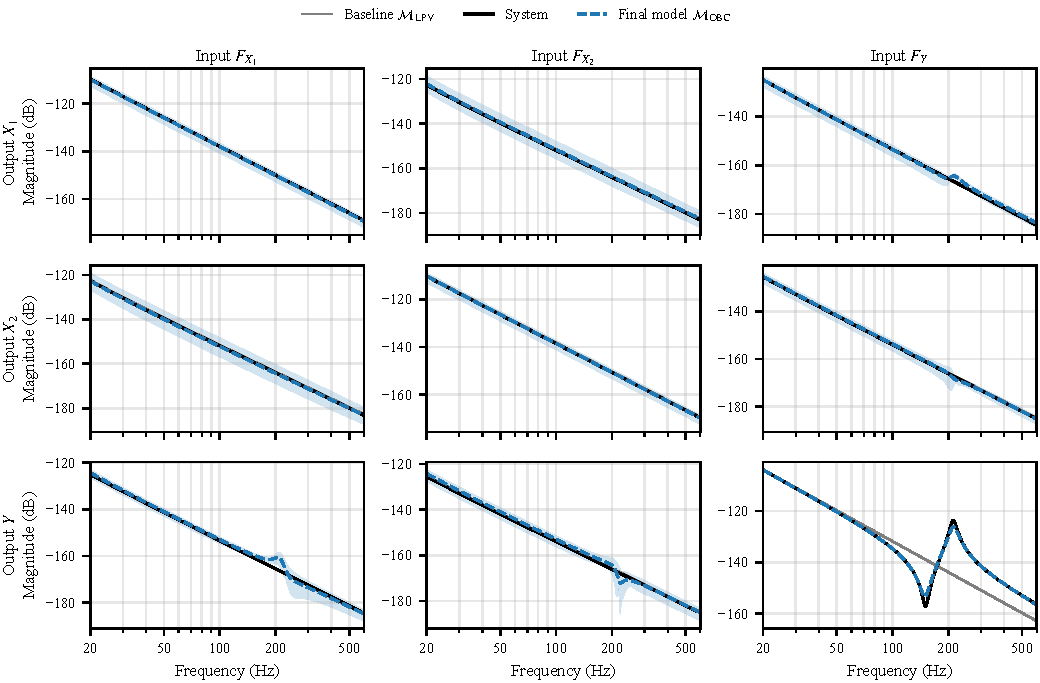
\includegraphics[width=\textwidth]{res_frf_full.pdf}
  \caption{Bode magnitude from the stage forces (columns) to the stage positions (rows), linearised at rest. Geometric mean over $Y=-0.39$ to $0.39$~m; shaded: range of the final model over $Y$.}
  \label{fig:res_frf_full}
\end{figure*}

\section{Experiment design details}\label{app:setup}
This appendix gives the details of Section~\ref{sec:setup} and the checks
of its design choices.
The checks use the known simulated system where the text says so.

\subsection{Data-generating system}\label{app:setup_system}
% Sources: vendor/ruleOfThumb.m, gtd_build_plant.m (K1); D-238, NOISE-INJECTION.md (noise).
\ifdraft
\begin{itemize}
\item The controller $K_1$ of every record
\item The noise spectrum, fitted to the standstill servo error of the machine (?: confidentiality)
\item The definition of the signal-to-noise ratio
\end{itemize}
\fi
The controller of every record is, per stage axis $j$,
\begin{equation}
 K_{1,j}(s)=\kappa_j\,\frac{s+\omega_b/6}{s}\,
 \frac{s+\omega_b/3}{s+3\omega_b}\,\frac{10\,\omega_b}{s+10\,\omega_b},
 \label{eq:setup_K1}
\end{equation}
where $\omega_b=2\pi f_b$ is the bandwidth and $\kappa_j$ sets the
open-loop gain of axis $j$ to one at $\omega_b$, for the diagonal entry of
the rigid baseline at $Y=0$ from stage force to stage position.
$K_1$ is discretised by the Tustin rule at $f_{\mathrm s}$.

The noise $v_j$ has the one-sided spectrum
\begin{equation}
 S_{v,j}(f)=\lambda_j^2\,\lvert H_j(f)\rvert^2+\sigma_{v,j}^2,
 \label{eq:setup_noise}
\end{equation}
where $H_j$ is a second-order Butterworth low-pass with cutoff $f_{v,j}$,
$\lambda_j$ its level and $\sigma_{v,j}$ a white floor.
$\lambda_j$ and $f_{v,j}$ are fitted so that the simulated standstill servo
error at $Y=0$ matches the measured one of the industrial machine, and
$\sigma_{v,j}$ is its level above 5~kHz.
The signal-to-noise ratio of Section~\ref{sec:setup_system} is
$\mathrm{SNR}_j=20\log_{10}\bigl(\mathrm{RMS}(y^{\circ}_j-r_j)/\mathrm{RMS}(y_j-y^{\circ}_j)\bigr)$
over the training records.

\subsection{Excitation and records}\label{app:setup_records}
% Sources: D-217, D-219 (band, grid, crest factor, amplitudes), MANIFEST (scale), Code/Setup band_frf.py,
% coverage.py; Code/Figures setup_band.py, setup_coverage.py.
\ifdraft
\begin{itemize}
\item The multisine: grid from the width of the anti-resonance, best crest factor of 30 draws, amplitudes, no record needed scaling
\item The upper band edge and the band over the frequency response of the simulated system
\item The five motion types, the operational moves and the operating range of all records
\end{itemize}
\fi
In each channel $c\in\{X,\Theta,Y\}$ of the generalised force, the
multisine is
\begin{equation}
 u^{\mathrm{ms}}_c(t)=A_c\sqrt{\frac{2}{\lvert\mathcal L\rvert}}\sum_{l\in\mathcal L}
 \cos(2\pi l\,\Delta f\,t+\alpha_{c,l}),
 \label{eq:setup_ms}
\end{equation}
where $\Delta f=0.005\,f_b$, $\mathcal L=\{212,\dots,594\}$ spans
$1.06\,f_b$ to $2.97\,f_b$, and the phases $\alpha_{c,l}$ are drawn uniformly per record.
It enters at the actuators as $u^{\mathrm{ff}}=P^{-1}u^{\mathrm{ms}}$.
The grid places 18 lines inside the half-power width $2\zeta_af_a=0.09\,f_b$ of
the anti-resonance, the narrowest feature of the system, and makes the
multisine periodic in 2~s.
Of 30 phase draws, the one with the lowest crest factor is kept; for $\Theta$
the crest factor is taken on the simulated yaw response.
The rms amplitudes $A_c$ keep every record within the force and stroke
limits of the machine without scaling.
$K_1$ is tuned for $f_b$ on the rigid baseline at $Y=0$.
On the simulated system, the crossover of the loop lies between
$\fpeval{round(\SetupCrossMin/100,2)}\,f_b$ and
$\fpeval{round(\SetupCrossMax/100,2)}\,f_b$ over the axes and the training
positions, so the band starts at the highest.
The upper edge follows from the best linear approximation of the simulated
system with friction under $K_1$, measured at the five training positions.
Above the crossover, the band holds 90\,\% of the squared difference between
this response and that of the baseline, counted where the difference
exceeds its uncertainty.
A rerun with the friction law of \eqref{eq:setup_fric} gives the same
edges.
\todo{Missing: reason for the 90\,\% share of the upper edge and for 30 phase draws, and a cite key for the best linear approximation. Candidate: keep both as heuristic (D-217, D-219); cite Pintelon and Schoukens 2012 for the best linear approximation (no cite key yet).}
\begin{figure}[t]
  \centering
  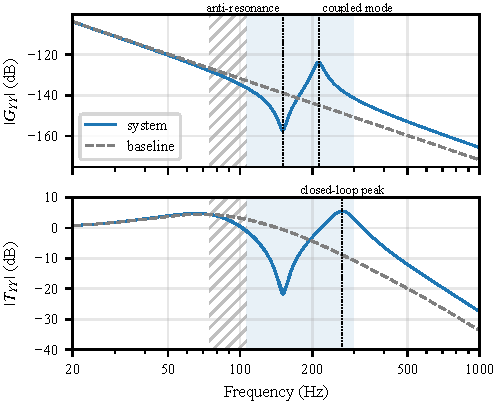
\includegraphics[width=\columnwidth]{setup_band.pdf}
  \caption{Stage axis $Y$ of the simulated system and of the baseline,
  linearised at the five training positions (lines overlap). Top: open
  loop. Bottom: complementary sensitivity with $K_1$. Shaded: multisine
  band; hatched: range of the $K_1$ crossovers over the axes and
  positions.}
  \label{fig:setup_band}
\end{figure}

The five motion types are standstill at a fixed $Y$, slow sweeps of $Y$,
$X$-$Y$ Lissajous paths, point-to-point moves with S-curve profiles, and
sine-shaped moves representative of machine operation.
The operational test records I3 to I6 are sine-shaped routes with $X$ and
$Y$ together, alternating $X$-only and $Y$-only moves, an S-curve route and
long strokes.
Table~\ref{tab:setup_records} lists the records, and
Fig.~\ref{fig:setup_coverage} shows their operating range.
\begin{table}[t]
\caption{Training, validation and test records.}
\label{tab:setup_records}
\centering
\footnotesize
\begin{tabular}{@{}lllll@{}}
\toprule
Record & Motion & Multisine & New & Pair\\
\midrule
Training & all five types & 14 of 18 & & \\
Validation & all five types & 4 of 6 & positions, draws & \\
\midrule
I1 & point-to-point & yes & phases, setpoints & \\
I2 & standstill & yes & position & \\
I3 & machine move & no$^\dagger$ & motion type & \\
I4 & route & no & motion type & \\
I5 & route & no$^\dagger$ & motion type & \\
I6 & route & no$^\dagger$ & motion type & \\
\midrule
E1 & standstill & yes & $\lvert Y\rvert=\fpeval{round(\SetupEY/\SetupTrainY,1)}\,Y_{\mathrm{tr}}$ & I2\\
E2 & machine move & no$^\dagger$ & stroke of $Y$ & I3\\
E3 & route & no$^\dagger$ & acceleration, \SetupEAcc\,\% & I5\\
E4 & route & no$^\dagger$ & velocity, \SetupEVel\,\% & I6\\
E6 & machine move & no$^\dagger$ & several, \SetupESixAcc\,\% acc. & I3\\
\bottomrule
\end{tabular}

\smallskip
\begin{minipage}{\linewidth}\footnotesize
I: interpolation, inside the training range. E: extrapolation, outside
it in the setting under New, with the motion of the Pair record. New:
what differs from the training records, for E from the Pair record.
E6 differs in more than one setting and is a stress record.
$^\dagger$Also evaluated with the training multisine added (I3M, E2M,
and so on), at equal amplitude within a pair and 0.30 of the training
amplitude for I6 and E4.
\end{minipage}
\end{table}
\begin{figure}[t]
  \centering
  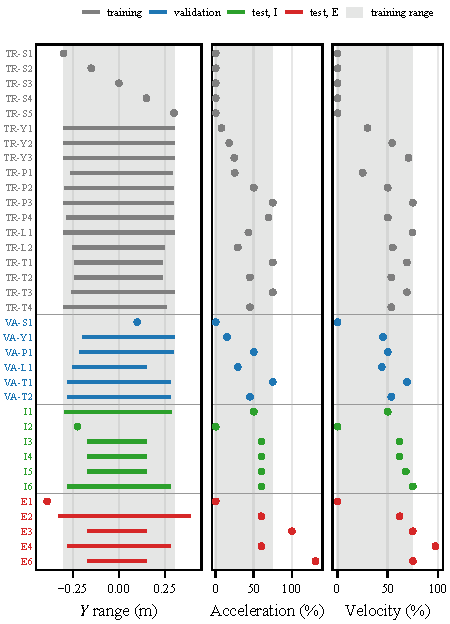
\includegraphics[width=\columnwidth]{setup_coverage.pdf}
  \caption{Range of $Y$ of each record against its largest acceleration
  (top) and velocity (bottom), in \% of the machine limits. Dashed: training
  range. Test records at the same level are offset by 4\,\% for
  legibility.}
  \label{fig:setup_coverage}
\end{figure}
\subsection{Processing and checks}\label{app:setup_checks}
% Sources: D-087 (block mean), D-166 (rate), D-220 (window), D-232 (filter), D-141 (controller rate);
% Code/Setup rate.py, filter_leak.py, filter_edge.py, loop_memory.py, controller_rate.py, rail_velocity.py.
\ifdraft
\begin{itemize}
\item The reduction to the model rate: block mean of the force, zero-phase filter on the servo error, trim at the record ends
\item The checks of rate, filter, window, controller rate and friction regime
\item The cause of the controller-rate change (?)
\end{itemize}
\fi
With the argument counting samples at $f_{\mathrm s}$, the records are
reduced to $T_s$ by
\begin{equation}
 u_k=\frac15\sum_{i=0}^{4}\uact(5k+i),\qquad
 y_k=r(5k)+\bigl(\mathcal B\ast(y-r)\bigr)(5k),
 \label{eq:setup_decim}
\end{equation}
where $\mathcal B$ is a zero-phase eighth-order Butterworth low-pass at
1.6~kHz.
The block mean is the exact input of a zero-order-hold model at $T_s$.
The filter acts on the servo error only, so the reference passes unchanged.
It changes the noise-free output by at most $\SetupFiltDist$~m RMS.
Its impulse response falls below 1\,\% of its peak within
\SetupFiltDecay~ms, so the \SetupTrim~ms removed at both record ends hold
its edge transient.
\todo{Missing: source for the cutoff at 0.8 times the Nyquist frequency and for the order 8. Candidate: Gautier, Janot and Vandanjon, IEEE TCST 2013 (decimation at 0.8 of the Nyquist frequency; no cite key yet); order 8 heuristic (D-232).}

For $\lvert v_i\rvert\ge3v_{\mathrm{fr}}$, the friction of
\eqref{eq:setup_fric} is within 0.5\,\% of the Coulomb law.
Table~\ref{tab:setup_checks} gives the checks of the design, including the
share of samples in this range.
\begin{table}[t]
\caption{Checks of the experiment design.}
\label{tab:setup_checks}
\centering
\footnotesize
\setlength{\tabcolsep}{3pt}
\begin{tabular}{@{}ll@{}}
\toprule
Check & Value\\
\midrule
\multicolumn{2}{@{}l}{\emph{Simulated loop, linearised at the training positions}}\\
Phase-margin loss, 4 / 2~kHz & \SetupPmLossFour$^\circ$ / \SetupPmLossTwo$^\circ$\\
Slowest closed-loop time constant & \SetupTauMax~ms\\
Response to a force error, 1\,\% & \SetupDecay~ms (window \SetupWindow~ms)\\
Filter impulse response, 1\,\% & \SetupFiltDecay~ms (trim \SetupTrim~ms)\\
\multicolumn{2}{@{}l}{\emph{Training records}}\\
Noise above 2~kHz, raw / filtered & $\SetupAliasRaw$ / $\SetupAliasFilt$~m\\
SNR $\fpeval{round(\SetupMotionFNN/100,2)}\,f_b$ to $1.05\,f_b$, without multisine & $\ge$\SetupGapSnrMinMotion~dB\\
Samples with $\lvert v\rvert\ge3v_{\mathrm{fr}}$, multisine & $\ge$\SetupRailShareMin\,\%\\
$K_1$ at 20~kHz, force error & $\SetupKcheck$\\
$K_1$ at $T_s$, force change, median & \SetupKmismatchMed\,\%\\
\quad largest; without multisine & \SetupKmismatchMax\,\%; \SetupKmismatchMotion\,\%\\
\bottomrule
\end{tabular}
\end{table}
The training loop re-discretises $K_1$ at $T_s$, which changes the feedback
force on the training records by a median of \SetupKmismatchMed\,\% RMS.
\todo{Missing: the cause of this change and whether it affects the results. Candidate: the half-sample offset between the block-mean force and the controller output at $T_s$ (2\,sin($\pi f\cdot0.1$~ms) is 9 to 19\,\% over the band, only records with multisine show it; not verified); the effect to Section~\ref{sec:results} or the Discussion.}
\revnote{Cause found (2026-10-16, D-265): the check compares the 4~kHz
controller output at sample $kD$ with the force averaged over $kD$ to $kD+4$,
centred 0.1~ms later. Compared at the same instant, the two controllers agree
to 0.5 to 1\,\% on TR-S1. The 10.8\,\% is the change of the force within one
0.25~ms hold, the cost of closing the loop at 4~kHz in simulation, not an
error in the block-mean preprocessing (D-087), which stays. Its output effect
is bounded by the oracle error of the closed-loop report. The check is
corrected to report both numbers separately, so these macros and this
sentence change.}

\subsection{Black-box model}\label{app:setup_bb}
% Sources: beintema2023subnet; scripts/gantry/blackbox-cl-trainable (train_bb_clmap.py), thesis_r8_grid.conf.
\ifdraft
\begin{itemize}
\item The SUBNET model of the closed loop, from reference and injected force to servo error, with its encoder
\end{itemize}
\fi
The black box of Section~\ref{sec:setup_models} is
\begin{equation}
 x^{\mathrm{bb}}_{k+1}=f_{\mathrm{bb}}\bigl(\theta_{\mathrm{bb}},x^{\mathrm{bb}}_k,r_k,u^{\mathrm{ms}}_k\bigr),\quad
 \hat y_k=r_k+h_{\mathrm{bb}}\bigl(\theta_{\mathrm{bb}},x^{\mathrm{bb}}_k\bigr),
 \label{eq:setup_bb}
\end{equation}
where $x^{\mathrm{bb}}_k\in\R^{n_x}$ and an encoder estimates
$x^{\mathrm{bb}}$ at the window start from past inputs and servo errors, as
in~\cite{beintema2023subnet}.
Its settings are the black-box rows of Table~\ref{tab:hyper}.

\subsection{Hyperparameters}\label{app:hyper}
Table~\ref{tab:hyper} lists the settings of every grey-box run and of the
black-box search.
The basis of a value is derived (computed in Section~\ref{sec:setup} or Appendix~\ref{app:setup}),
inherited (from earlier work), tuned (on validation data), heuristic (fixed
without a measurement) or compute-limited.
\begin{table}[t]
\caption{Hyperparameters of the identification.}
\label{tab:hyper}
\centering
\footnotesize
\setlength{\tabcolsep}{3pt}
\begin{tabular}{@{}lll@{}}
\toprule
Setting & Value & Basis\\
\midrule
\multicolumn{3}{@{}l}{\emph{Model and data}}\\
Model rate $1/T_s$ & 4~kHz & derived\\
RK4 steps per $T_s$ & 1 & heuristic\\
Window $n_f$ & 400 (0.1~s) & derived\\
Window stride & 10 samples & heuristic\\
Encoder window $n+1$ & 30 samples & heuristic\\
Added states $n_{\bar x}$ & 0, 2, 8 & compared\\
Network, encoder correction & $2\times16$, tanh & tuned (earlier)\\
Precision & float64 & numerical\\
Margin $\gamma$ & 0.99 & heuristic\\
Detuning of the combinations & 10\,\% & heuristic\\
\multicolumn{3}{@{}l}{\emph{Optimiser}}\\
Adam rate, $\epsilon$ & $10^{-5}$, $10^{-16}$ & tuned (earlier)\\
Batch & 512 windows & heuristic\\
Epochs & 200 & compute-limited\\
Validation interval & 1300 updates & compute-limited\\
L-BFGS iterations, history & 100, 50 & inherited\\
L-BFGS inner steps, windows & 20, 16384 & compute-limited\\
L-BFGS tolerance (grad., change) & $10^{-12}$, 0 & inherited\\
Seeds per model & 1 & compute-limited\\
\multicolumn{3}{@{}l}{\emph{PS (Section~\ref{sec:aug_ps2}, Appendix~\ref{app:ps_stop})}}\\
S1 and S2 Adam rate & $10^{-3}$ & Adam default\\
S1 batch, windows $\lvert\mathcal C\rvert$ & 64, 128 & heuristic\\
Decoder width $n_h$, horizon $H$ & 16, $n+1$ & as above\\
Check interval $i_c$ & 25 updates & heuristic\\
Plateau checks $w$, tolerance $\delta_\nu$ & 4, 0.02 & heuristic\\
S1 updates $i_{\min}$, $i_{\max}$ & 100, 350 & heuristic\\
Early check $i_s$, threshold $\nu_{\max}$ & 150, 0.90 & heuristic\\
Held-out records & last per class & heuristic\\
S2 pairs $N_{\mathcal P}$ (fit, held-out) & 8192, 2048 & heuristic\\
S2 batch, check interval & 512, 100 updates & heuristic\\
S2 plateau (checks, tolerance) & 5, 0.01 & heuristic\\
S2 updates (min, max) & 500, 8000 & heuristic\\
\multicolumn{3}{@{}l}{\emph{Black box (Section~\ref{sec:setup_models})}}\\
States $n_x$ & 8, 16, 32 & tuned\\
Width of $f_{\mathrm{bb}}$, $h_{\mathrm{bb}}$ (encoder $2\times$) & 8, 16, 32 & tuned\\
Adam rate & $10^{-3}$, $3\cdot10^{-3}$, $10^{-2}$ & tuned\\
Batch, stride & 256, 25 & inherited\\
Updates (search, final) & 20000, 80000 & compute-limited\\
Selection & lowest validation RMS & heuristic\\
\bottomrule
\end{tabular}
\end{table}
\revnote{Final runs, rows to update: L-BFGS tolerance (grad., change)
$2.6\times10^{-5}$, $2.6\times10^{-7}$ (D-263, production ratio to the
weighted loss); held-out records: last per class with at least 3 records;
black box: all 11 configurations to 80000 updates, objective and selection on
validation NRMS$_e$ (D-264). New row, encoder start: least squares of
\cite[Eq.~(33)]{hoekstra2026encoder}, the numerical-rank-truncated SVD
solution in standardised regressors, cutoff $\max(N,m)\,\epsilon$ (the
PyTorch default), convention (D-271).}
\todo{Missing: a stated reason for the rows marked heuristic without one in \texttt{docs/decisions.md} (window stride, batch, RK4 steps, the PS rules). Candidate: keep them as heuristic, with D-234 as the source of the PS rules (prototype runs).}
\todo{Missing: the black-box rows are the search grid of \texttt{thesis\_r8\_grid.conf}; the selected configuration is not known yet. Candidate: add a row with the selected $n_x$, width and rate once R8 has run.}

\begin{wip}
\subsection{OBC and experiment details}
\begin{itemize}
\item Derive the stacked projector, rank-deficient pseudoinverse case, epoch refresh, and additional-state zero extension
\item Derive $J^+\Delta^*$ and list the measured singular-direction contributions to the predicted parameter bias
\item List dataset identifiers, split membership, hyperparameters, seed, and exact metric definitions for every reported arm
\item Figure (existing, optional): place \texttt{controller-chain-v1} here only if the controller reconstruction cannot be audited adequately in prose and equations
\end{itemize}
\todo{Can code and data tables be cited through a repository or DOI instead of spending paper space on full reproducibility metadata?}
\end{wip}


\end{document}
